%+--------+
%| HEADER |
%+--------+

\documentclass[12pt,twoside,openright]{book}

%%%Packages
\usepackage[T1]{fontenc}
\usepackage[utf8]{inputenc}
\usepackage{cite}
\usepackage[titletoc]{appendix}
\usepackage[font=small]{caption}
%\usepackage[font=footnotesize]{caption} % even tinier, just in case...
    \captionsetup{font={stretch=1}}
\usepackage{setspace}
    \setstretch{1.2}

% Presentation and structure
\usepackage{hyperref}
    %\usepackage[hidelinks]{hyperref} %Without link border...
\usepackage{graphics,graphicx}
    \DeclareGraphicsExtensions{.pdf,.png,.jpg}
\usepackage{rotating, float}
\usepackage{afterpage}
\usepackage{caption}
\usepackage{subcaption}
\usepackage{color}
\usepackage[table,xcdraw]{xcolor}
    \definecolor{mygrey}{RGB}{233,233,233}
    \definecolor{myred1}{HTML}{CF2C1D}
    \definecolor{myred2}{HTML}{D76536}
    \definecolor{myora1}{HTML}{DC9056}
    \definecolor{myora2}{HTML}{E0B77D}
    \definecolor{mywhit}{HTML}{E0DCAE}
    \definecolor{myaqu2}{HTML}{9ABBA1}
    \definecolor{myaqu1}{HTML}{679789}
    \definecolor{mygre2}{HTML}{3E726E}
    \definecolor{mygre1}{HTML}{174F52}
    \definecolor{mygri1}{RGB}{206,210,211}
    \definecolor{mygri2}{RGB}{228,230,230}
    \definecolor{mynavi}{RGB}{79,95,98}
\usepackage{tabularx}
\usepackage{multicol}
\usepackage{multirow}
\usepackage{longtable}
\usepackage{arydshln}
    \setlength{\dashlinedash}{3pt}
    \setlength{\dashlinegap}{4.5pt}
    \setlength{\arrayrulewidth}{0.2pt}
\usepackage{imakeidx}
    %\usepackage{nature}

% Various
\usepackage{lipsum}
\usepackage{kantlipsum}
\usepackage{pdfpages}
\usepackage{enumerate}
\usepackage{enumitem}
\usepackage[intoc]{nomencl}
\usepackage{setspace}
\usepackage{anyfontsize}
\usepackage[nottoc,numbib]{tocbibind}

% Titles and aesthetic
\usepackage{titlesec}
\titleformat{\chapter}[display]
    {\normalfont\bfseries}{}{0pt}{\fontsize{40}{50}\selectfont}
\usepackage{emptypage}
%\usepackage{lmodern}

% Margins and Text
\usepackage{geometry}
\geometry{
	total={210mm,280mm},
	left=30mm,
	right=30mm,
	bindingoffset=0mm,
	top=30mm,
	bottom=30mm
}

% Custom footers and headers
\usepackage{fancyhdr}
\pagestyle{fancy}
    \renewcommand{\chaptermark}[1]{ \markboth{#1}{} }
    \renewcommand{\sectionmark}[1]{ \markright{#1}{} }
    \fancyfoot[LE,RO]{\thepage}
    \fancyfoot[CE,CO]{}
    \fancyhead[LE,RO]{\leftmark}
    \fancyhead[RE,LO]{\rightmark}
    \renewcommand{\headrulewidth}{0.4pt}
    \renewcommand{\footrulewidth}{0pt}
\fancypagestyle{plain}{
    \fancyfoot[LE,RO]{\thepage}
    \fancyhead[LE,RE,RO,LO]{}
    \renewcommand{\headrulewidth}{0pt}
    \renewcommand{\footrulewidth}{0pt}
}

% Drawing
\usepackage{tikz}
\usetikzlibrary{positioning}
\usetikzlibrary{shapes.geometric, arrows}
\tikzstyle{software} = [rectangle, minimum width=2cm, minimum height=0.7cm, text centered, draw=black, fill=mynavi, text=white]
\tikzstyle{input} = [rectangle, minimum width=2cm, minimum height=0.5cm, text centered, draw=myora1, fill=mygri2, text=black]
\tikzstyle{output} = [rectangle, minimum width=2cm, minimum height=0.5cm, text centered, draw=myora1, fill=mygri1, text=black]
\tikzstyle{midput} = [rectangle, minimum width=2cm, minimum height=0.4cm, text centered, text=myora1]
\tikzstyle{flow} = [dashed,thick,->,>=stealth,myora1]
\tikzstyle{inout} = [thick,->,>=stealth,myora1]

% Commands and names
\renewcommand{\figurename}{Fig.}
\newcommand{\quotes}[1]{``#1''}
\newcommand{\lline}{\rule{\linewidth}{0.5pt}}
\newcommand{\blankpage}{
    \newpage
    \thispagestyle{plain}
    \mbox{}
}
\newlength\longest
\renewcommand*{\arraystretch}{1.1}

\renewcommand{\nomname}{List of Abbreviations}

\newcommand{\hsap}{\texttt{hsap}, \textit{H. sapiens}}
\newcommand{\bacu}{\texttt{bacu}, \textit{B. acutorostrata}}
\newcommand{\bmys}{\texttt{bmys}, \textit{B. mysticetus}}
\newcommand{\mmon}{\texttt{mmon}, \textit{M. monoceros}}
\newcommand{\dleu}{\texttt{dleu}, \textit{D. leucas}}
\newcommand{\ttru}{\texttt{ttru}, \textit{T. truncatus}}
\newcommand{\oorc}{\texttt{oorc}, \textit{O. orca}}
\newcommand{\pmac}{\texttt{pmac}, \textit{P. macrocephalus}}
\newcommand{\mmus}{\texttt{mmus}, \textit{M. musculus}}
\newcommand{\ggal}{\texttt{ggal}, \textit{G. gallus}}
\newcommand{\acar}{\texttt{acar}, \textit{A. carolinensis}}
\newcommand{\psin}{\texttt{psin}, \textit{P. sinensis}}
\newcommand{\cpic}{\texttt{cpic}, \textit{C. picta belli}}
\newcommand{\gaga}{\texttt{gaga}, \textit{G. agassizii}}
\newcommand{\agig}{\texttt{agig}, \textit{A. gigantea}}
\newcommand{\cabi}{\texttt{cabi}, \textit{C. abingdonii}}
\newcommand{\cmyd}{\texttt{cmyd}, \textit{C. mydas}}

%%% Data
\title{Comparative analysis of the Degradome in long lived Metazoans}
\author{Jos\'{e} Mar\'{i}a Gonz\'{a}lez P\'{e}rez-S\b{i}lva}
\date{October, 2020}

\makenomenclature

%+------+
%| BODY |
%+------+

\begin{document}
\raggedbottom % Remove if extreme ugliness is caused by different textheights in different pages... 

\frontmatter
\pagestyle{empty}

\cleardoublepage
\newgeometry{top=1.5cm,left=2cm,right=2cm,bottom=1.5cm}

\begin{figure}[t]
    \begin{center}
        %\includegraphics[width=0.4\columnwidth]{figures/logo_color_centrado.pdf}
        \includegraphics[width=0.4\columnwidth]{figures/logo_verde_centrado.pdf}
        %\includegraphics[width=0.6\columnwidth]{figures/logo_color_izquierda.pdf}
        %\includegraphics[width=0.6\columnwidth]{figures/logo_verde_izquierda.pdf}
        \caption*{}
    \end{center}
\end{figure}

\begin{center}

\large
\textbf{Programa de Doctorado en Biomedicina y Oncolog\'{i}a Molecular}

\vspace*{1.5cm}

\fontsize{35}{45}
\textbf{Comparative analysis of the Degradome of long-lived metazoans}

\vspace*{3cm}

\huge
\textbf{Doctoral Thesis}

\vspace*{\fill}

\large
Jos\'{e} Mar\'{i}a Gonz\'{a}lez P\'{e}rez-Silva

October, 2020
\end{center}

\restoregeometry

\cleardoublepage
\includepdf[pages={-}]{autorization_to_present.pdf}
\includepdf[pages={-}]{resolution_to_present.pdf}
\includepdf[pages={-}]{summary.pdf}

\cleardoublepage
%\thispagestyle{plain}
\thispagestyle{empty}
%\begin{flushright}
\begin{itshape}
\small

    Esta tesis es la culminación de varios años de trabajo, pero, más aún, representa la síntesis de una etapa de mi vida, y como tal, además de recoger en ella los resultados y conclusiones de los proyectos en que he participado, es necesario dedicar también unas frases a todas las personas que, de una u otra forma, han contribuido a que este barco llegue a buen puerto.

    Por ello, y en primer lugar, quiero agradecer a Carlos la oportunidad que me dio de empezar todo esto una tarde extremadamente cálida, hace ya muchos años. Gracias, Carlos, por apostar por mí en una situación en que muchos otros no lo habrían hecho, por abrirme las puertas al que, desde siempre, había sido mi sueño.
    
    Gracias a Víctor, por introducirme en el mundo de la bioinformática, por su dirección y tutela cuando necesité guía, y por dejarme espacio para crecer independientemente cuando la situación lo permitía. Gracias por tu paciencia, Víctor, sé que no siempre fue fácil.
    
    Gracias a Gloria, a Josemari, y a Xose, porque sin ellos el laboratorio no sería lo que es, por cuidar de todos nosotros en las buenas y en las malas, por su preocupación y dedicación constante. Gracias por vuestra implicación y dedicación. Gracias también a Yaiza, que con su trabajo hace el de los demás más fácil. Gracias por intentar animarnos y ayudarnos siempre.
    
    Gracias a todos los compañeros de laboratorio, con los que tantas horas he compartido. Gracias por toda la ayuda prestada y por tantos buenos ratos, por los cafés, las conversaciones, y por tantas tardes de sesiones músicales.
    
    Thanks to Dr. Kevin Howe for letting me visit his lab for three wonderful months. Thank you for your help and willingness. Thanks also to Fergal and his team (especially to Leanne), for your patience, your advice and guidance, and for making me feel welcomed and \emph{cozy}. You helped me to learn a different way of doing science and for that I'm (again) grateful.
    
    Y por supuesto, gracias a la Universidad de Oviedo, al Instituto Universitario Oncológico del Principado de Asturias, y al ministerio de Salud por su continuado apoyo financiero y sus ayudas durate la realización de esta tesis.

    \bigskip
    
    Pero no todo iba a ser trabajar, así que tengo que dedicar unas palabras de agradecimiento especial a un grupo que pese a haber nacido entre las paredes del labo, ha trascendido con creces a lo largo de los años. Gracias a las personas que pasaron de no atreverse a compartir coche en un viaje de 200 kilómetros a venirse conmigo al otro lado del globo. No son palabras vacías si os digo que sin vosotros esto no habría sido posible. No solo por el constante apoyo y los buenos momentos, sino por compartir los malos (y los muy malos). Por todas las fiestas, las \quotes{autoinvitaciones}, los viajes y las escapadas, mil gracias.
    
    Gracias también a mi \quotes{cohorte de Sandramandra}, gracias por haber estado ahí desde tiempos inmemoriales. Por las innumerables horas de aventuras imaginarias en tierras desconocidas, por todas las visitas (casi improvisadas) a mi país adoptivo, las reuniones (algo más planificadas) en el país bávaro, y los (de momento inexistentes) viajes a las tierras de la lengua incomprensible. Y, por supuesto, por las \quotes{tertulias científicas} durante las noches de vermú. Gracias por todo.
    
    A mi \quotes{equipo de IT}, gracias. Gracias por que con vuestros chistes y provocaciones me disteis la determinación que necesitaba para avanzar en un campo que me era desconocido, y con vuestros consejos y eterna disposición, me ayudasteis a progresar en el mismo. Gracias por estar \quotes{aquí}, por las noches de peli, por las sesiones de turismo de \quotes{aperitivo}, por los campings y por todos los buenos momentos.

    No puedo terminar sin darle las gracias a mi familia, por su constante e incondicional apoyo. A mis padres, sin quienes no habría llegado tan lejos. Gracias por llevarme a la universidad, por ayudarme a avanzar curso a curso, y por seguir a pie del cañón día a día. También a mi hermana, compañera en muchos viajes (no solo de carretera), a mis tíos y tías, por vuestro interés en mi trabajo y vuestros ánimos, a mis primos por todos los buenos ratos de esparcimiento, y, de una forma muy especial, gracias a mis abuelas, por todo vuestro apoyo y amor.

    \bigskip

    Finalmente, me gustaría dedicarle la presente tesis a mis abuelos Paco y Pepe, que de una forma u otra me han inspirado a tomar este camino y han hecho que me sienta orgulloso de haberlo seguido. Gracias por ayudarme a estar aquí hoy.

\end{itshape}
%\end{flushright}


\cleardoublepage
\thispagestyle{plain}
\null\vfill
\settowidth\longest{\Large\itshape except in the light of evolution.}
\begin{center}
    \parbox{\longest}{
        \raggedright{\Large\itshape
        Nothing in biology makes sense \\
        except in the light of evolution.\par\bigskip}   
        \raggedleft\large\MakeUppercase{Theodosius Dobzhansky}\par
    }
\end{center}
\vfill\vfill

\tableofcontents
\listoffigures
\listoftables
\printnomenclature[2cm]

\mainmatter
\pagestyle{fancy}

\chapter{Introduction}

%In his Inaugural Lecture at University College London, Dr. Peter B. Medawar defined for the fist time \textsl{ageing} as merely surviving the years, ignoring the increased deterioration and decay. 
%He proposed at the same time to use the word \textsl{senescence} for those processes, stating that it should mean decline of vitality \cite{Medawar1952}.
%Interestingly, he made these definitions in his lecture \quotes{An Unsolved Problem in Biology}, also remarking how much things had changed in 50 years in terms of mortality.
%Dr. Medawar noticed how the principal causes of death shifted from infective towards cancer and cardiovascular diseases, both with a certain genetic susceptibility.
%And so, a basis for considering ageing as subjected to the forces of Natural Selection was established.
%Not many years later, in 1958, Theodosius Dobzhansky defined ageing as the decline of homoeostasis, linking it again to the affairs of natural selection.
%This definition is much closer to the one we work with currently, whereby ageing is the decay of biological fitness, which in itself refers to an evolutionary term.

In 1958, Theodosius Dobzhansky published an essay discussing the relation between homoeostasis and senility, and how natural selection affects both \cite{Dobzhansky1958}.
On it, Dobzhansky reflected on the concept of homoeostasis, defined by Walter Cannon some years before as the \quotes{wisdom of the body} \cite{Cannon1934}, or the ability to, through controlled changes in the organism, adapt to changes in the eviroment, provided that they are within the \quotes{normal} changes the organism had evolved to withstand.
He also linked this concept with ageing, by defining the later as the reduction of this adaptability or plasticity agains \quotes{normal} enviromental changes.
Specifically, he proposed that \quotes{\textsl{the homeostatic buffering against enviromental shocks is weakened during the postreproductive phase}}.

In his work \quotes{The Causes of Evolution}, Haldane considered this topic without any clear conclusion.
To him, natural selection \quotes{may either favor or hinder the prolongation of life during the postreproductive phase} \cite{Haldane1933}.
To Dobzhansky, the fact that homoeostatic mechanisms \quotes{tend to deteriorate during the autumm of life}, while the same function most efficiently during youth and maturity, is indication of how these are fashioned by natural selection.
Of course, we now understand in much more detail how far the link between homoeostasis and ageing goes, knowing specific cell paths, cellular systems, and other homoeostasis mechanisms for which \emph{heritable} malfuction (or even slightly under-optimal function) is a cause for a hastened ageing process.

After decades of tentative work on these determinants of ageing, in 2013, a seminal work finally established a precise framework to study how genetic determinants and their interaction with the environment regulates this process \cite{Lopez-Otin2013}. 
The framework is based on nine \emph{hallmarks of ageing}.

\section{Hallmarks of ageing} \label{s_intro_hallmarks}

Ageing is quasi-universal among multicellular organisms, yet, it is probably one of the least-understood of the natural processes of our biology \cite{Kirkwood2005}.
It can be described as a progressive loss of biological fitness, or the progressive decline in functional integrity and homoeostasis, culminating in death \cite{Singh2019}.
As such, it is expected to be caused by a continuous accumulation of damage with points of inflexion, at which the attempts of the body of fighting this creeping decay adds to the deleterious nature of ageing.

The characterization of the hallmarks of ageing, much like what happened with the hallmarks of cancer previously published \cite{Hanahan2011}, has helped conceptualize the underlying nature of ageing whilst setting a frame in its study.

For its categorization, each hallmark must satisfy 3 key principles:

\begin{enumerate}[topsep=1ex,itemsep=-1ex]
    \item It should manifest under normal ageing.
    \item Its experimental aggravation should accelerate the normal ageing process.
    \item Its experimental betterment should delay the normal ageing process, increasing healthspan and lifespan.
\end{enumerate}

Following this canon, nine hallmarks were defined.
These were genomic instability, telomere attrition, epigenetic alterations, loss of proteostasis, deregulated nutrient sensing, mitochondrial dysfunction, cellular senescence, stem cell exhaustion, and altered intercellular communication.
These nine hallmarks were grouped in 3 categories, depending on their impact on the process of ageing.
The first category, \emph{primary hallmarks}, is composed of those considered to be the causes of cellular damage, including genomic instability, telomere attrition, epigenetic alterations, and loss of proteostasis.
The second category, (\emph{antagonistic hallmarks}), was defined as the group of compensatory or antagonistic responses to the damage produced by the primary hallmarks.
While these responses are able to initially mitigate the damaging effects produced by the primary hallmarks, after becoming chronic they will turn deleterious as well.
This group includes deregulated nutrient sensing, mitochondrial dysfunction, and cellular senescence.
Lastly, \emph{integrative hallmarks}, which arise from the consequences of the previous groups, are directly responsible for the functional decline associated with ageing.
This category consists of two hallmarks, stem cell exhaustion, and altered intercellular communications \cite{Lopez-Otin2013}.

\begin{figure}[t!]
    \begin{center}
        \includegraphics[width=\textwidth]{figures/hallmarks.pdf}
        \caption[The hallmarks of ageing]{\footnotesize The nine hallmarks of ageing, grouped by category using the different colours.
        In \textcolor{myred1}{\textbf{red}} are displayed the primary hallmarks, such as genomic instability, telomere attrition, epigenetic alterations, and loss of proteostasis.
        In \textcolor{myora1}{\textbf{orange}} we can see the secondary or antagonistic hallmarks, \textit{i.e.} deregulated nutrient sensing, mitochondrial dysfunction, and cellular senescence.
        Finally, those in \textcolor{myaqu1}{\textbf{green}} are the integrative hallmarks, namely, stem exhaustion, and altered intercellular communication.}
        \label{f_hallmarks}
    \end{center}
\end{figure}

\subsection{Primary hallmarks} \label{ss_intro_hallmarks_primary}

\emph{Genomic instability} refers to the gradual accumulation of genetic damage throughout life \cite{Moskalev2013}.
As we age, the integrity and stability of our DNA\nomenclature{DNA}{Deoxyribonucleic Acid} is being continuously challenged by both exogenous and endogenous threats.
Physical, chemical and biological agents such as  ultraviolet light, mutagenic substances, or even viral replication are some examples of exogenous damage that DNA must withstand.
In addition, DNA faces internal sources of instability, such as replication errors, or the damage produce by some by-products of our own metabolism, like ROS\nomenclature{ROS}{Reactive Oxygen Species} \cite{Hoeijmakers2009}.
Overall, the genome is constantly suffering highly diverse lesions, including point mutations, translocations, chromosomal gains and losses, telomere shortening, and gene disruption caused by the integration of viruses and transposons.
For that reason, organisms have evolved a complex network of DNA repair mechanisms capable of tackling most of this problems \cite{Lord2012}.
Excessive DNA damage, or insufficient DNA repair favours the ageing process.
On the other hand, incorrect handling of this repair process is in itself one of the sources of further damage to the DNA.
Thus, many lesions are originated after mismatch repair, non-homologous end-joining, translesion synthesis, or base excision repair \cite{Agathangelou2018}.
Hence, these aquired complex systems and characteristics are subject to heredity and hence to the forces of natural selection, adding weight to the hypothesis of heritable longevity \cite{Lord2012}.

The aforementioned damage to the DNA is seemingly random in location, but there are some specific chromosome regions that are specially susceptible to age-related dam\-age, such as the telomeres.
Telomeres, a genomic region made up of repeated sequences at the end of each chromosomal arm, are among such regions, making \emph{telomere attrition} another primary hallmark.
This reduction in length that accompanies ageing originates from the natural incapability of the DNA polymerase to completely replicate the terminal ends of linear DNA molecules \cite{Turner2019}.
There is a specific DNA polymerase capable of replicating this \quotes{caps}, known as telomerase, but it is not expressed by most of mammalian cell types, leading to the progressive reduction of this DNA segment over time \cite{Shay2016}.
Researchers have observed not only a natural reduction of telomere size during normal ageing, but also that the pathological dysfunction of telomerase in experimental models greatly accelerates the process of ageing.

As we advance in the field of epigenetics, we increasingly recognise the importance of its physiological and pathological role in a lot of different biological processes, including ageing.
For this reason, we include \emph{epigenomic alterations} as one of the primary hallmarks of ageing.
These modifications affect all cells and tissues throughout life, via DNA methylation, post-translational modification of histones, and chromatin remodelling, and can be linked to accelerated ageing processes \cite{Pal2016}.
For instance, it has been experimentally observed that specific epigenetic alterations can mimic progeroid syndromes in model organisms\cite{Osorio2010}.
%Furthermore, enhancing the epigenetical function of SIRT6 has shown to increase the healthy lifespan, while decreasing it seems to diminish longevity \cite{Kanfi2012}.
Because of this, understanding and manipulating the epigenome holds promise for improving age-related pathologies, hence extending lifespan and, more importantly, healthspan.

The last primary hallmark of ageing, \emph{loss of proteostasis}, relates to the maintenance of a correct protein homoeostasis in the cell, meaning, getting rid of defective proteins, or correcting them.
The function of most proteins depends on their tridimensional structure, hence a misfolded protein could either not have function at all or have a different, unregulated one.
Specifically, we use the term \quotes{proteostasis} to reffer collectively to all the paths that deal with unfolded or misfolded proteins, namely the autophagy path, proteasome and lysosome degradation paths, and refolding via chaperones \cite{Klaips2018}.
These paths can be regulated based on the action of the heat-shock protein family \cite{Hartl2011,Koga2011,Mizushima2008}.
%Whenever these paths suffer alterations, unfolded or misfolded proteins remain in the cell and tend to aggregate, generating pathologies and hastening ageing.
In a normal situation, the different pathways works coordinatedly towards restoring the structure of misfolded peptides or to remove and degrade them completely, avoiding the accumulation of damaged (and damaging) proteins \cite{Powers2009}.
Numerous studies have shown that ageing tends to alter proteostasis, decreasing its effectiveness \cite{Hipp2019}.
When this happens, it has been observed that chronic accumulation of misfolded proteins may lead to age-related pathologies, such as Alzheimer and Parkinson's disease, or cataracts \cite{Powers2009}.
Finally, when inducing perturbations in this system, age-associated pathologies as well as hastened ageing has been observed.
In contrast, by improving proteostasis we can achieve the opposite effect and delay ageing \cite{Zhang2008}.

\subsection{Antagonistic hallmarks} \label{ss_intro_hallmarks_secondary}

The \emph{deregulation of nutrient sensing} hallmark relates to the system that detects and corrects the levels of different nutrients, energy, and other elements that alter body homoeostasis.
This complex hallmark stems from the relationship between anabolic signalling and accelerated ageing \cite{Fontana2010}.
As an example of this, a pharmacological manipulation that mimics low availability of nutrients has been observed to extend longevity in mice \cite{Harrison2009}.
Also, consistent with this, dietary restriction has shown to increase healthy lifespan in several species, including some primates \cite{Mattison2017}.
% Demasiado escueto? Es un tema un poco complejo para entrar a saco pero igual podemos mencionar algo de la glucosa? O será meterse en un maizal?

Ageing also affects the respiratory chain, whose efficacy diminishes with age, increasing electron leakage and reducing ATP\nomenclature{ATP}{Adenosine TriPhosphate} generation \cite{Green2011}.
We know this hallmark as \emph{mitochondrial dysfunction}.
In turn, these problems tend to increase the concentration of ROS, which, as mentioned before, also plays an important role in accelerating ageing \cite{Harman1965}.
While this association between defects in the respiratory chain and hastened ageing has being known for a long time, major details remain a research challenge.
In fact, the fulfilment of the third principle of hallmarks (amelioration leading to higher lifespan) is still under discussion.

\emph{Cellular senescence} is defined as a stable arrest of the cell cycle coupled with phenotypic changes \cite{Campisi2007,Kuilman2010}.
Several ageing-related stimuli are believed to trigger this process, including telomere shortening, non-telomeric DNA damage, and depression of the INK4/ARF locus \cite{Collado2007}.
The accumulation of senescence cells in a tissue can be indirectly measured through surrogate markers, such as DNA damage or the presence of metabolites such as senescence-associated $\beta$-galactosidase \cite{Dimri1995}.
It has been observed that these senescent cells are not equally accumulated across tissues in old age.
In fact, some organs, like heart or kidney, do not show changes in senescence associated to age \cite{Hoenicke2012,Kang2011,Xue2007}.
It has been widely assumed that senescent cells contribute to ageing, however, cellular senescence should be considered a response from the body to ageing, by marking cells for their deletion.
Sadly, as we age, due to all the other problems associated, the mechanisms that should get rid of these \quotes{marked} cells function suboptimally, and the deletion does not happen as fast as it should (or at all) \cite{Calcinotto2019}.
Therefore, it is the process of ageing which promotes the accumulation of senescent cells that otherwise should have been killed and removed.
Thus, the malfunction of the turnover system that replaces cells in tissues lowers the regenerative capacity of the progenitor cells and leads to their exhaustion.

\subsection{Integrative hallmarks} \label{ss_intro_hallmarks_integrative} %actualizar referencias

As we previously stated, these hallmarks are the direct result of the previous ones.
Its chronification is the final cause for most of the phenotypic changes associated with ageing.
And so, as a direct response to cellular senescence, the first of these hallamarks is \emph{stem cell exhaustion}.
It can be defined as the decline in the regenerative potential of tissues.
For instance, it has been shown that haematopoietic stem cells of aged mice decrease in cell-cycle activity compared to those of young mice \cite{DeHaan2018,Shaw2010}.
Of course, this directly correlates with a higher accumulation of DNA damage and over-expression of cell-cycle arrest proteins such as p16\textsuperscript{INK4a} \cite{Janzen2006,Rossi2007,Stenvinkel2017}.
While a deficit in proliferation is detrimental for the long-term maintenance of the organism, its excess is equally damaging, since it translates into an early exhaustion of the proliferating capacity of the stem cells of the tissue.
This effect has been observed in experiments with \textit{Drosophila melanogaster} intestinal stem cells, where excessive proliferation lead to exhaustion and premature ageing \cite{Rera2011,Wang2014}.
As an integrative hallmark, stem-cell exhaustion can be modulated by interventions on primary and antagonistic hallmarks.
For instance, it has been shown that inducing \textit{INK4a} (related to cellular senescence), or decreasing IGF-1 (related to deregulated nutrient sensing), we can help preserve the quiescence of stem cells, delaying stem cell exhaustion in the organism \cite{Chakkalakal2012,Tumpel2019}.

Besides cell-autonomous alterations, ageing also involves changes at the level of cell-cell integration, either by endocrine, neuronal or neuroendocrine paths \cite{Laplante2012,Rando2012,Zhang2013}.
Thus, \emph{altered intercellular communication}, the last hallmark of ageing, has ubiquitous effects in several different signalling paths, including a deregulation in neurohormonal signalling (such as renin-angiotensin, adrenergic or insulin-IGF1 signalling) \cite{Bocheva2019}.
This provokes an increase in inflammatory reactions, a decrease in immunosurveillance against both pathogens and premalignant cells, and also changes in the composition of the peri- and extracellular environment.
One of the most interesting effects of an altered intercellular communication is a smouldering proinflammatory phenotype associated with ageing called \emph{inflammageing} \cite{Franceschi2014}.
Inflammaging has different causes, such as an accumulation of proinflammatory tissue damage, a failure of an immune system to effectively clear pathogens or dysfunctional cells, propensity to secrete proinflammatory cytokines by senescent cells, or an autophagic response \cite{Franceschi2017,Salminen2012}.
% Lo mismo que en derregulation of nutrient sensing... Dado que es uno de los que luego tienen mas importancia en cachalote y tortuga, debería explayarme algo más?

%\subsection{Ageing as a progressive loss of function decline} \label{ss_intro_hallmarks_ageing}
%
%Having stabilised the main routes affected by longevity, I'd like to further discuss how this process takes place, by progressively increasing the difficulty in maintaining the homoeostasis. [Something on those lines, \cite{Kirkwood2005} may be useful].

\section{The Degradome}

As clearly reflected by the hallmarks of ageing, ageing is an extremely complex trait, with multiple intertwined systems, and a network of causes and consequences that extend to almost any remarkable cellular pathway.
A useful step in tackling these complexities is to separate a simpler system that nevertheless recapitulates some of the characteristics of the whole system.
In this regard, we have extensively worked on \emph{proteases}, \textit{i. e.}, proteins capable of degrading other proteins by means of peptide bond hydrolysis in an essentially irreversible way \cite{Perez-Silva2015}.
Proteases influence diverse biological features of the organisms, such as the immune system, digestion process, skin regeneration, cell cycle progression, tissue remodelling, neuronal outgrowth, haemostasis, wound healing, angiogenesis, apoptosis or metastasis, \cite{Lopez-Otin2008,Quiros2015,Reinhard2015,Voskoboinik2015}.

Due to these ubiquitous functions, the proper function of the proteolytic system is key to maintain homoeostasis in the organism, so it must be tightly regulated in terms of both activation and specificity.
Failings in their regulation underlie very diverse pathological conditions, such as progeria, cancer or even mental illness\cite{Turk2012}.
Thus, this set of genes experienced a remarkable evolutive expansion as an adaptation to regulate the large set of substrates depending on its correct functioning.

The large number of protease genes \cite{Perez-Silva2015} and their interdependence led to the definition of the \emph{degradome} as the complete set of proteases in a given organism \cite{Lopez-Otin2002a}.
The set of techniques that study and characterise proteases in this context is known as \emph{degradomics}. 
Given the large amount of information we often work with when delving in degradomics, bioinformatic techniques are important tools, as they allow researchers to focus on the biological meaning of the data and not its processing. 
Our experience and the mining of literature are usually a vital complement to the manual curation of annotations after automatic predictions and other analysis.
All together aimed towards finding links between protease alterations and pathological consequences, including hereditary diseases, sometimes referred as \emph{degradomopathies} \cite{Quesada2009}

\section{Molecular strategies against ageing and model organisms} \label{s_intro_models}

With information on hallmarks of ageing and the influence of proteases on them, we can look for clues on how longevity affects the genome of long lived animals.
The abundant data on protease function and biochemistry can then be leveraged to discern some of the molecular mechanisms that underlie extended life-span.
As controls, we can use evolutionary comparison with both close and distant relatives of diverse longevity.

\subsection{\textit{Physeter macrocephalus} and other Cetacea} \label{ss_intro_models_sperm_whale}

The sperm whale is a marine mammal, part of the Cetacea infraorder.
As such, they are part of the order Artiodactyla\footnote{Sometimes referred as Cetartiodactyla, a combination of \quotes{Cetacean} and \quotes{Artiodactylia}, arguing that despite the clear evidence supporting this clade, the enormous morphological differences between cetaceans and the rest justify this distinction.} (also known as even-toed ungulates), placing them as relatives to Camelidae (suborder Tylopoda), the pig and close family (suborder Suina), the ruminants (suborder Ruminantia), and hippopotamuses (with whom Cetacea share the Whippomorpha suborder; figure \ref{f_cetacean_tree}) \cite{Agnarsson2008}.
Cetacea and Sirenia (the order of manatees or sea cows) are the only mammals that live their entire lives inside the water.
Interestingly, they are not closely related to those, nor to Superfamily Pinnipedia (seals and the like), the only other mammal adapted to semiaquatic life \cite{Arnason2007,Tabuce2008}.
This suggests that aquatic adaptation developed independently several times in Mammalia, an example of convergent evolution.
On its own, Cetacea is further divided into two parvorders, Odontoceti, to which the sperm whale belongs, and Mysticeti \cite{Mancia2018}.

\textsl{Mysticeti} or \quotes{Baleen Whales} feed on plankton, by using a filter-like system based on extremely thin keratin bristle-like structures called baleen (as in its \quotes{common} name \cite{Fordyce2018}.
The fifteen members composing this parvorder are quite diverse, ranging in size from the 6 $m$ and 3,000 $kg$ of the pygmy right whale to the 31 $m$ and 190,000 $kg$ of the blue whale \cite{Agnarsson2008,Wada2003}.
They also diverge in other features, such as life expectancy and diving capacity.
Of special interest in the present work is the Bowhead whale (\emph{B. mysticetus}), some of whose specimens have been shown to live over 400 years, the largest life span recorded among Mammalia \cite{Keane2015}.
In addition, the availability of genomic data on Minke whale (\emph{B. acutorostrata}) allows genetic comparisons, as both whales are representatives of the Mysticeti parvorder \cite{Yim2014c}.

\textsl{Odontoceti} or toothed whales, are those presenting teeth.
These cetaceans feed on meat from various species, from aquatic mammals to fishes, including, in the case of the sperm whale, giant squids \cite{Best1979}.
As found in the parvorder of the Mysticeti, there is great divergence between members of this group as well, with species ranging from 1.5 $m$ and 50 $kg$ to more than 20 $m$ and 50,000 $kg$ \cite{Warren2017a}.
Odontoceti is a much larger parvorder than Mysticeti, with more than 70 different species \cite{Agnarsson2008}.
As a reflection of this diversity, Odontoceti are further divided in \textsl{Physeteroidea}, the superfamily comprising the sperm whales and relatives; \textsl{Delphinoidea}, including all salt-water dolphins and relatives (\textit{e.g.}, the killer whale, or the \textsl{Monodontidae} family, composed of narwhals and beluga whales); \textsl{Ziphioidea}, the superfamily of the beaked whales (\textit{e.g.}, Cuvier's whale); and 3 other superfamilies that include the fresh-water dolphins, \textsl{Inioidea}, \textsl{Platanistoidea}, and \textsl{Lipotoidea} (figure \ref{f_testudines_tree}) \cite{Agnarsson2008}.
In terms of longevity this parvorder is also diverse, featuring species with life-spans that range from 20 to 100 years, the maximum life expectancy for a sperm whale \cite{Whitehead2003}.

Sperm whales are believed to posses great cognitive capacities.
Not only do they have the largest brain on earth, but also present complex social behaviours.
They take care as a group of calves and elderly, protecting wounded or weaker individuals from predators, and they migrate as organised groups \cite{Best1979}.
One of their most salient features is their echolocation apparatus, which in fact originated the name \emph{sperm whale}.
The peculiar shape of the cranium of these animals allows the allocation of a waxy substance inside it, the spermaceti\footnote{Called 'spermaceti' after wrongly assuming the function that it played in sperm whale biology.} \cite{Alam2016,Clarke1970}.
The spermaceti, whose function is still partly unclear, is though to provide the internal needed resonation that allows these whales to use a sophisticated system of communication based on ultrasounds (\emph{clicks}) \cite{Mohl2001}.
This is key to their cognitive development and their social behaviour, since these clicks are supposed to be used for a variety of reasons.
Thus, not only do sperm whales use echo location in the dark depths, but also, according to some researchers, they are able to perform some 'low-level' communication between them using this system, to the point of assigning specific names to members of the family \cite{Schulz2011}.
It was believed that another use of these clicks was to \quotes{stun} prey during hunting, but it has been  proven that while useful in the chase and to buzz them, there is no stunning involved \cite{Fais2016}.

\begin{figure}[t!]
    \begin{center}
        \includegraphics[width=0.9\textwidth]{figures/spermaceti.pdf}
        \caption[Spermaceti organ]{\footnotesize Outline of the spermaceti organ and the craneum architecture of the sperm whale. Both the spermaceti and the sponge-like melon are thought to participe in the complex resonance system described. Adapted from \textsl{WikiCommons}, Creative Commons license.}
        \label{f_spermaceti}
    \end{center}
\end{figure}

As a member of one of the few groups of mammals solely living in aqueous environments (Cetacea), sperm whales have undergone a process of adaptation to underwater distinctive features.
First and foremost, given the nature of water, gravity is much more forgiving with organisms, allowing them to reach larger sizes, which grant these creatures a series of attributes.
Thus, a link between longevity and size was already hinted by Aristotle in the \textsl{IV} century BC \cite{Speakman2005}. 
This link is particularly apparent in the case of Bowhead whales who, as we mentioned before, can live to up to 4 centuries.
In addition to that, as dictated by Peto's paradox, the observation of a moderate frequency of cancer occurrences in this gargantuan animals suggests extremely tight cancer protection mechanisms.
Namely, by virtue of having a very large body, cetaceans are made of a larger number of cells than other mammals, which means more cells potentially able to develop cancer-like mutations.
Therefore, this increase in cell number must be compensated by a much lower probability for tumorigenesis in each cell, accomplished via different systems \cite{Tollis2017a}.
Secondly, changes in pressure from shallow to deep waters demand different ways of regulation of blood homoeostasis (also known as \emph{haemostasis}) \cite{Stewart2009}.
This is especially important in the case of sperm whales, which, along with the Cuvier's whale, is one of the deepest divers known among mammals \cite{Schorr2014}.

On top of all of these features, sperm whales develop a distinctive skin structure, presenting a significant thicker \textsl{stratum corneum} than that of other Cetacea.
In addition to the tissue structure of the skin, it differs macroscopically from other cetaceans in which it is more wrinkled (sometimes it is compared to a raisin).
Also, sperm whales shed skin more regularly than other species \cite{Sokolov1982}.
Given the fact that skin is the first line of defence against the environment, these special traits may provide some advantage to the sperm whale in terms of physical defence, both against the attacks of their prey and the medium itself.
Thus, it has been proposed a relationship between the diving peculiarities of the sperm whale and those of its skin, maybe also weighting in its hunting habits \cite{Strauss1969}.

\subsection{Lonesome George and other giant tortoises} \label{ss_intro_models_giant_tortoises}

On September of 1835, \textsl{HMS Beagle} arrived to the shores of the Gal\'{a}pagos Archipelago to perform cartography mappings.
For some weeks, on-board naturalist and geologist Charles Darwin also observed and recollected data on the island biodiversity, which, eventually, along with other findings, helped him enact his theory of evolution by means of natural selection.
Among these observations, he noticed that the tortoises from different islands displayed conspicuous differences.
Even so, tortoises from the same island presented very diverse shells depending on the altitude of their habitat \cite{Darwin1845}.
Ever since, partly due its implication in the development of this theory, the Gal\'{a}pagos giant tortoises have become well known everywhere, and have greatly contributed to the well-deserved notoriety of the archipelago.
The most famous Gal\'{a}pagos tortoise was Lonesome George, the last member of his species, \textit{Chelonoidis abingdonii}, who tragically died in 2012, when believed to be ~101-102 years old, becoming an important symbol for conservation efforts, both in the Gal\'{a}pagos Islands and around the world.

At some point it was considered that all Gal\'{a}pagos tortoises were, in fact, one single species, \textit{Chelonoidis nigra}, composed of several subspecies (\textit{e.g.}, Lonesome George would have belonged to the subspecies \textit{C. nigra abingdonii}) \cite{Caccone1999}.
Nowadays, studies support the idea of several differentiated species, sharing the same genus (\textit{Chelonoidis}), but each independent \cite{Le2006}.

\begin{figure}[t!]
    \begin{center}
        \includegraphics[width=1\textwidth]{figures/galapagos.pdf}
        \caption[Gal\'{a}pagos giant tortoises and their habitat]{\footnotesize Representation of the Gal\'{a}pagos Island (names in \textbf{black}) and the Gal\'{a}pagos giant tortoises that inhabits them, indicating in \textcolor{myred1}{\textbf{red}} those that are currently extinct, in \textcolor{myora1}{\textbf{orange}} those in doubt, and in \textcolor{mygre2}{\textbf{green}} the rest. Adapted from \textsl{WikiCommons}, Creative Commons license.}
        \label{f_galapagos}
    \end{center}
\end{figure}

As a group, these species are all part of the class Reptilia (also referred to as Sauropsida).
Reptilia is a complex clade, since we must contemplate that birds are part of it in order to considerate it a monophyletic group, or to assume that it's paraphyletic (leaving crocodiles on a side).
The traditional approach went by considering 2 subdivision of this class, Diapsida, and Anapsida, which refers to the number of openings in their skulls (Diapsida having two of them, and Anapsida having none).
This classification,based on directly observable morphological features, has been revised and the current approach consist on 2 subdivisions as well, this time being Eureptilia, and Parareptilia \cite{Benton2014}.
While Parareptilia is extinct, Eureptilia contains itself another subdivision, called Diapsida, in which diapsides have being merged with anapsides, that has being rename as infraclass Neodiapsida.
Inside this infraclass, Testudinata constitutes an order on its own, while Lepidosauromorpha (Tuataras, lizards, and snakes) and Archosauromorpha (crocodiles and birds, along with dinosaurs), maintain their status of infraclasses (figure \ref{f_testudines_tree}) \cite{Mannen1999,Modesto2004}.

Turtles\footnote{Disclaimer: \quotes{Turtle} can refer to the order as a whole or, when differentiating between them, to the aquatic Testudines. In this sense, we use \quotes{tortoises} to refer to the land members of the order, while those able of both walking and swimming will be referred at as \quotes{terrapins}. Whenever talking about the specific varieties we will try to stick to the more specific names possible.} comprises more than 300 species \cite{Rhodin2017}.
This group is subdivided into two suborders, Pleurodira and Cryptodira, depending on whether their neck retracts sidewards or backwards, respectively.
The extant members of Pleurodira are largely restricted to fresh-water ecosystems \cite{Ferreira2018}. 
On the other hand, Cryptodira thrive in land, aquatic and mixed habitats.
They present different adaptations according to feeding, both herbivorous and carnivorous, not to mention sizes, ranging from some centimetres to more than 2 metres.
%Interestingly, many of the larger species have been reported to present a gigantism not linked to island gigantism\footnote{A phenomena by which an isolated specie tends to increase or reduce its size depending on his original inland size being small or big (respectively), by means of redistribution of tropic relations in the island ecosystem.}.

Another remarkable feature of turtles is their longevity.
Allegedly, one of the oldest turtles to ever live, \textsl{Adwaita} an Aldabra giant tortoise (\textit{A. gigantea}), reached more than 250 years.
Sadly no records are kept to support this claim.
Among those with recorded or tested age, \textsl{Tu'i Malila} (deceased in 1956) and \textsl{Jonathan} (still alive) are both 188 years old and are thus considered the longest lived terrestrial animals.
Notably, while \textsl{Jonathan} is also an Aldabra tortoise, \textsl{Tu'i Malila} was a member of \textit{Geochelone radiata}, one of the land relatives of Gal\'{a}pagos Giant tortoises (of a much smaller size).
Next in the list would be \textsl{Harriet}, a Gal\'{a}pagos giant tortoise (\textit{C. porteri}), who died in 2006 at the age of 176 years.
Another small tortoise, \textsl{Timothy}, lived 160 years, from around 1844 to 2004.
Timothy belonged to \textit{Testudo gracea}, also related to the land family of Gal\'{a}pagos giant tortoises.
In this sense, it has been discussed that the \quotes{early} dead of Lonesome George had some pathological component to it, but this doesn't make his age negligible.

%To cite other interesting characteristics in tortoises, it has been noted from an early time their capability to enter an \quotes{stasis} state, similar to hibernation, in which they can survive for almost a year without nutrients or water.
%For this reason they were used as a naturally preserved source of food in the long ship trips, including that of \textsl{H.M.S. Beagle}.
%Also, almost as a curiosity, in some zoological publications of the XIX century, a researcher reported movement and activity up to more than 15 days after surgically removing the head. 

\bigskip
\bigskip
\bigskip
All these long-lived metazoans must show genomic footprints of the evolutionary processes that lent them a combination of molecular characteristics that solve the problems associated with longevity.
With the intention of shedding some light on the subject of ageing, and to contribute to the collective efforts in solving this impending problem, the present Doctoral Thesis aims to study some of nature's solutions from an evolutionary point of view, paying special attention to the study of the degradome and its impact on longevity.

\vspace*{\fill}

\begin{sidewaysfigure}[ht!]                                                                    
    \begin{center}                                                                             
        \includegraphics[width=\textwidth]{figures/cetacean_tree.pdf}                          
        \caption[Cetacea taxonomy tree]{\footnotesize Cetacea taxonomy tree, including the rest of families composing the order Artiodactyla (denoted by the \textcolor{mygre2}{green} point). Marked in \textcolor{myora1}{orange} those specifically referred to in the text and hence used in the comparison studies. Marked with an asterisk are those which annotation is part of the work presented in this thesis, although punctual annotations for specific genes in the rest were also performed. Based in the relations shown by \quotes{Time tree} \cite{Kumar2017}.}
        \label{f_cetacean_tree}                                                                
    \end{center}                                                                               
\end{sidewaysfigure}                                                                          

\begin{sidewaysfigure}[ht!]
    \begin{center}
        \includegraphics[width=0.9\textwidth]{figures/testudines_tree.pdf}
        \caption[Testudines taxonomy tree]{Testudines taxonomi tree, including the rest of species used in the comparative studies as representatives of the main families comprising the clade of Sauropsida, and \textit{H. sapiens} as the out-group an and reference. Marked in \textcolor{myora1}{\textbf{orange}} are those annotated as part of the present thesis, although punctual annotations for specific genes in the rest were also performed. Closely related tortoises both continental and from the Gal\'{a}pagos archipelago are indicated with the \textcolor{mygre1}{\textbf{darker green}} point, while the radiation of island tortoises is marked using the \textcolor{myaqu1}{\textbf{lighter green}}. Based on the relations shown by \quotes{Time tree} \cite{Kumar2017}.}
        \label{f_testudines_tree}
    \end{center}
\end{sidewaysfigure}


\chapter{Objectives}

Taking into consideration both the previous work in the field and the experience of our laboratory in degradomics, in this thesis we aimed to annotate, analyse and compare proteases and other genes in the genomes of long-lived metazoans.

Thus, the specific objectives for this Doctoral Thesis were:

\begin{enumerate}[topsep=1ex,itemsep=1ex]
    \item Study and analysis of \textsl{Physeter macrocephalus}'s Degradome.
    \begin{enumerate}[label=\arabic{enumi}.\arabic*,itemsep=0ex]
        \item Manual annotation of \textsl{P. macrocephalus}'s Degradome.
        \item Comparison of this gene set with that of the other annotated marine mammals (i.e. Bowhead whale, Minke whale, Bottlenose dolphin, and Killer whale).
        \item Study of the differences and similarities in an evolutionary context.
    \end{enumerate}
    \item Study and analysis of \textsl{C. abingdonii}'s Degradome.
    \begin{enumerate}[label=\arabic{enumi}.\arabic*,itemsep=0ex]
        \item Manual annotation of \textsl{C. abingdonii}'s Degradome.
        \item Comparison of this gene set with that of the other annotated tortoises (i.e. other Giant Galapagos tortoises, continental relatives, and Aldabra tortoise).
        \item Study of the differences and similarities in an evolutionary context.
    \end{enumerate}
    \item Study and analysis of other genomic families of interest in \textsl{C. abingdonii}.
    \begin{enumerate}[label=\arabic{enumi}.\arabic*,itemsep=0ex]
        \item Automatic annotation of the complete genome of \textsl{C. abingdonii}.
        \item Study of the evolutionary traits of the different families.
        \item Study of the genomic variation of gene families of interest among related species.
    \end{enumerate}
\end{enumerate}


\chapter{Materials and methods}

\section{Molecular biology methods} \label{s_matmet_molecular}

\subsection{Data collection} \label{ss_matmet_molecular_data_colection}

\subsubsection*{Sperm whale} 

Tissue samples were obtained from an adult female specimen found in the northern Gulf of Mexico.
DNA was then extracted with the DNAeasy kit from Quiagen, according to the manufacturer's protocol. 
RNA samples were collected from skin tissues (n=5) also from other specimens at the Gulf of Mexico using Trizol reagent (Invitrogen) according to the manufacturer specifications.
RNA quality was assessed by electrophoresis using an Agilent 2100 Bioanalyzer (Santa Rosa, CA).
Additional samples from four different individuals were extracted from \quotes{Voyage of the \textsl{Odyssey} samples} using a high-salt procedure \cite{Godard2003}.
The gender of each specimen was determined based on amplification by PCR of the \textit{SRY} gene \cite{Richard1994}.

\subsubsection*{Gal\'{a}pagos giant tortoise}

Both DNA and RNA samples from \textit{C. abingdonii} were recovered from a frozen sample of blood belonging to Lonesome George.
In parallel, we obtained samples of a granulome in an individual of \textit{A. gigantea} from which we extracted DNA and RNA. % Está apuntado en la libreta de Olaya...
Samples for PCR and Sanger sequencing were obtained from an array of samples provided by Yale University.

\subsection{Genome sequencing} \label{ss_matmet_molecular_genome_sequencing}

\subsubsection*{Sperm whale}

Library collections for genome assembly consisted of paired-end (200 bp), and mate-pair libraries (insert sizes: 3, 8, and 40 kbp). All libraries were sequenced using paired 100 bp reads on an \textsl{Illumina HiSeq2000} ultrasequencer.
Additional samples were sequenced to medium depth (~20-30X) by sequencing paired-end short insert libraries (~300bp) to 125bp length on an \textsl{Illumina Hi-Seq X10} instrument.
All RNAseq data are available through the NCBI SRA, under BioProject number \href{https://www.ncbi.nlm.nih.gov/bioproject/177694}{PRJNA177694}%(\href{https://www.ncbi.nlm.nih.gov/bioproject/PRJNA177694}{www.ncbi.nlm.nih.gov/bioproject/PRJNA177694}).
.

\subsubsection*{Gal\'{a}pagos giant tortoises}

Library collections built for sequencing on the \textsl{Illumina Hi-Seq 2000} platform, from a 180 bp-insert paired-end library, a 5 kb-insert mate-pair library and a 20 kb-insert mate-pair library.
Additionally, reads from 18 PacBio SMRT\textsuperscript{TM} cells were used to extend the contigs.
For the DNA sample from Aldabra tortoise we used Illumina technology and a 180 bp paired-end library to obtain whole-genome data.
All the reads are available under BioProject number \href{https://www.ncbi.nlm.nih.gov/bioproject/416050}{PRJNA416050}%(\href{https://www.ncbi.nlm.nih.gov/bioproject/416050}{www.ncbi.nlm.nih.gov/bioproject/416050}).
.

\subsection{RNA sequencing} \label{ss_matmet_molecular_rna_sequencing}

\subsubsection*{Sperm whale}

RNAseq paired-end data (100 bp length) were generated from Illumina TruSeq cDNA (stranded) libraries using the Hi-Seq 2000 instrument. %Tissues? Alignment software?: Lo que sabemos de los tejidos está en data collection, lo del alineamiento que sabemos en la parte de alineamiento... Si no está ahí es que el paper no lo dice...
All RNAseq data are available through the NCBI SRA, under BioProject number \href{https://www.ncbi.nlm.nih.gov/bioproject/PRJNA177694}{PRJNA177694}.

\subsubsection*{Gal\'{a}pagos giant tortoise and other tortoises}

RNAseq paired-end data were generated from Illumina TruSeq libraries using the Hi\-Seq\-2000 instrument.
All the reads are available under BioProject number \href{https://www.ncbi.nlm.nih.gov/bioproject/416050}{PRJNA416050}.

\subsection{Gene selection} \label{ss_matmet_molecular_gene_selection}

Whenever manual annotation of genes was performed, the first step would be to select the set of genes to annotate.
In the cases in which the target set to annotate is the Degradome, an already curated database is prepared.
In other cases, genes were chosen after extensive literature mining using our experience in the field of ageing.
In the case of Lonesome George, more than 3,000 genes were chosen by this method.
This number includes the more than 600 genes that comprise the Degradome.
Unless otherwise noted, the sequences of all starting gene sets are taken from the human genome.

\section{Bioinformatics methods} \label{s_matmet_bioinformatics}

\subsection{Genome assembly} \label{ss_matmet_bioinformatics_genome_assembly}

\subsubsection*{Sperm whale}

The combined sequence reads were assembled with the AllPaths software \cite{Butler2008} using default parameter settings.
This draft assembly was gap-filled with a version of Image \cite{Tsai2010} that was modified for large genomes, and cleaned of contaminating contigs by performing a MegaBLAST \cite{Zhang2000} of the contigs against bacterial and vertebrate genome databases.
Contigs that displayed the best alignment over 50\% of their length with a different species were removed.
Using a genome size estimate of 2.8 Gbp, the total raw sequence depth of Illumina reads was > 90X.
The final sperm whale genome assembly was repeat-masked using WindowMasker \cite{Morgulis2006}.

\subsubsection*{Gal\'{a}pagos giant tortoise}

The assembly of these libraries was performed with the AllPaths algorithm \cite{Butler2008} to yield a draft genome of 64,657 contigs with an \emph{N50} of 74 kb (Table \ref{t_george_statistics}).
Then, we scaffolded these contigs using Sspace (v3.0) \cite{Boetzer2014a} employing the long-insert mate-pair libraries.
Finally, we filled the gaps using PBJelly (v15.8.24) \cite{English2012} and the reads obtained from 18 PacBio cells.
The final assembly (\textsl{CheloAbing 1.0}) was 2.3 Gb long.
Over this final assembly, we soft-masked repeated regions with RepeatMasker \cite{Smit} using a database of chordate repeated elements (provided by the software) as reference.
We then aligned the resulting reads to the \textit{C. abingdonii} assembly with BWA (v0.7.5a) \cite{Li2009}.
Similarly, raw genomic reads from \textit{C. abingdonii} were aligned to \textsl{CheloAbing 1.0} for manual curation purposes.

\begin{figure}[!t]
	\centering
	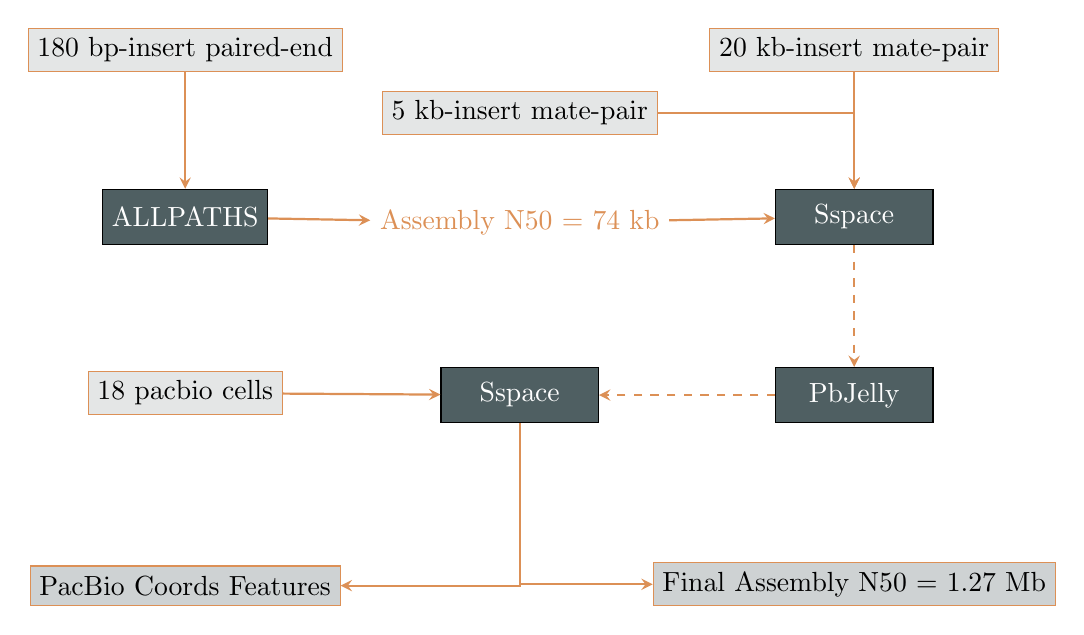
\begin{tikzpicture}[align=center,node distance=2cm]
	\node (b)[]{};
	\node (a)[left=4cm of b]{};
	\node (c)[right=4cm of b]{};
	\node (180)[input, above=3cm of a]{180 bp-insert paired-end};
	\node (5)[input, above=2.2cm of b]{5 kb-insert mate-pair};
	\node (20)[input, above=3cm of c]{20 kb-insert mate-pair};
	\node (pb)[input, below=0.55cm of a]{18 pacbio cells};
	\node(allpaths)[software, above=0.8cm of a]{ALLPATHS};
	\node(sspace)[software, above=0.8cm of c]{Sspace};
	\node(pbjelly)[software, below=0.5cm of c]{PbJelly};
	\node(sspace2)[software, below=0.5cm of b]{Sspace};
	\node(contigs)[midput, above=0.8cm of b]{Assembly N50 = 74 kb};
	\node(feapb)[output, output, below=3.02cm of a]{PacBio Coords Features};
	\node(assembly)[output, below=2.98cm of c]{Final Assembly N50 = 1.27 Mb};
	\draw [inout] (180) -- (allpaths);
	\draw [inout] (allpaths) -- (contigs);
	\draw [inout] (contigs) -- (sspace);
	\draw [inout] (20) -- (sspace);
	\draw [inout] (5) -| (sspace);
	\draw [inout] (pb) -- (sspace2);
	\draw [flow] (sspace) -- (pbjelly);
	\draw [flow] (pbjelly) -- (sspace2);
	\draw [inout] (sspace2) |- (feapb);
	\draw [inout] (sspace2) |- (assembly);
	\end{tikzpicture}
	\caption[Assembly process in Lonesome George's project]{\footnotesize Assembly process in Lonesome George's project.}
	\label{f_assembly_george}
\end{figure}

\subsection{RNA mapping and assembly} \label{ss_matmet_bioinformatics_rna_assembly}

\subsubsection*{Gal\'{a}pagos giant tortoises}

We aligned RNA-Seq data from \textit{C. abingdonii} blood and \textit{A. gigantea} granuloma to the assembled genome using TopHat (v2.0.14) \cite{Trapnell2009}.

\subsection{Genome completeness assessment} \label{ss_matmet_bioinformatics_genome_completeness}

The relative completeness in terms of expected gene content of the assembled genomes and their annotated gene sets was assessed using the Benchmarking Universal Single-Copy Ortholog (BUSCO) assessment tool \cite{Seppey2019}.

\subsubsection*{Sperm whale}

In the case of the sperm whale, we used the laurasiatheria\_odb9 lineage dataset that contains 6253 BUSCOs (v3.0.0).
The dependencies used were Augustus v3.2.3, and HMMER v3.1b1 \cite{Eddy2011}.

\subsubsection*{Gal\'{a}pagos giant tortoise}

In this case the program was run from an all-dependencies included Ubuntu virtual machine (available in \href{https://busco-archive.ezlab.org/}{https://busco-archive.ezlab.org/}).
For this assessment, we used the vertebrata\_odb9 lineage dataset.
We performed this analysis \textit{de novo} in CH38 human's assembly, to compare between them.
Additionally, by using the published data of the Mojave dessert tortoise, we increase the scope of the comparison.

\subsection{Genome automatic annotation} \label{ss_matmet_bioinformatics_automatic_annotation}

\subsubsection*{Gal\'{a}pagos giant tortoise}

We performed de novo annotation on the genome assembly of \emph{C. abingdonii} using \emph{MAKER2}, a multi-threaded, parallelized computational tool designed to produce accurate annotations for novel genomes based on a machine-learning approach \cite{Campbell2014}.
We fed the algorithm with both the \textsl{CheloAbing 1.0} assembly and the RNA-Seq data, as well as reference genome sequences from human and \emph{P. sinensis}.
We also provided multifasta files of the complete annotated set of human and \emph{P. sinensis} proteins.
With this input, MAKER2 completed two runs in a Microsoft Azure virtual machine.
Finally, predicted genes were assigned a putative function as part of the MAKER2 pipeline.

\subsubsection*{EBL-EBI annotation pipeline} \label{sss_matmet_bioinformatics_automatic_annotation_ebi}

In the automatic annotation process of the narwhal and the beluga whale, during my short internship in the European Bioinformatic Institute, I used a different approach.
In its first step, this method takes advantage of the data repository inside ENSEMBL. Thus, the pipeline automatically searches for all the evidence used in the annotation process.
The algorithm accepts a unique accession number for the assembly.
By using the data associated to said number in the SQL databases, it finds and uses any RNASeq information available.

From this point on, a program which works on top of a LSF\nomenclature{LSF}{Load Sharing Facility} (a job scheduler), manages a swarm of scripts, each of which takes care of one part of the annotation process.
They work on general tasks, such as the masking of the genome or the generation of an index, but also more annotation-related tasks, such as model generation, or comparison among related organisms.
Finally, by using the main annotation softwares, such as Geneblast or Augustus, and comparing the results between all of them and also with the RNASeq-generated models, a final set is generated.
This set is then manually revised to check for anomalies that may indicate a poorly performed annotation.
In addition, the researcher is tasked with controlling the correct performance of the pipeline by checking guiHive, a program designed to graphically show the steps of the annotation, current state, several inputs, outputs and options of each step, and the warnings and errors produced in the annotation. 

\subsection{Manual genome annotation} \label{ss_matmet_manual_annotation}

Manual annotation is largely based on the search for orthologs of our genes of interest in the genome of the species we want to annotate.
The most commonly used tool for this task is \emph{BLAST}\nomenclature{BLAST}{Basic Local Alignment Search Tool} \cite{Altschul1990}, an alignment algorithm designed to compare different sequences of nucleotides or amino acids.
This alone would yield a low-quality set of annotated proteins, since, given the own bias of the aligner, there will be some errors in the sequence, specially in the exon-intron junction sequences.
In order to correct the predicted alignment and assure the proper genetic structure, further steps are required.
These steps of manual curation can be tedious and error-prone. To make the task easier and safer, we performed all manual annotations using the BATI\nomenclature{BATI}{Blast Annotate Tune and Iterate} algorithm, developed in this laboratory.

The main ideas behind this pipeline are to perform all alignments automatically, to provide a graphical environment to easily correct said alignments, and to summarize all the results in a comprehensive format that allows the user to effortless point out duplicates or new genes.
This is achieved through four independent programs, that, once initialized, can be simultaneously used by several researchers working in the same set without conflicting each other's work.
These scripts are written in Perl v5 and can be obtained from our group web site (\href{http://degradome.uniovi.es/downloads.html}{http://degradome.uniovi.es/downloads.html}).

\begin{enumerate}[topsep=1ex,itemsep=-1ex]
	\item{\texttt{tbex     }} The first script to be executed. It prepares all required files and runs all the \texttt{tblastn} comparisons.
	\item{\texttt{bgmix    }} Summarizes all the hits from the different \texttt{tblastn} results in one single file.
	\item{\texttt{bsniffer }} Generates a file per model gene, containing the \texttt{tblastn} result in a more readable format for users to choose.
	\item{\texttt{genetuner}} Provides a graphical environment in which we can adjust intron-exon junctions and add or remove sequence stretches.
	\item{\texttt{bgmix    }} Non-redundantly summarizes all the \texttt{tblastn} hits, highlighting those belonging to an annotated gene. This allows the user to quickly find further copies of the genes under study.
\end{enumerate}

\texttt{tbex} has two functions.
The first one consists of creating a file containing the necessary data for the pipeline (\textit{i.e.} the genome of the organism we want to annotate, the protein sequence of the genes we are interested in annotate, and, optionally, the cDNA of said sequences, all in fasta format).
The genome must be indexed. If necessary, the script itself will run \texttt{formatdb} on it.
Once this is complete, the script will launch an instance of BLAST for each protein sequence we have given it.
Specifically, the flavour of BLAST used is \texttt{tblastn} (as \texttt{blastall -p tblastn}, which will search the protein sequence given in a translated version of the nucleotidic genomic sequence.
This flavour was chosen because evolutive pressures on genes are more evident on the protein sequence.

\begin{figure}[!t]
	\centering
	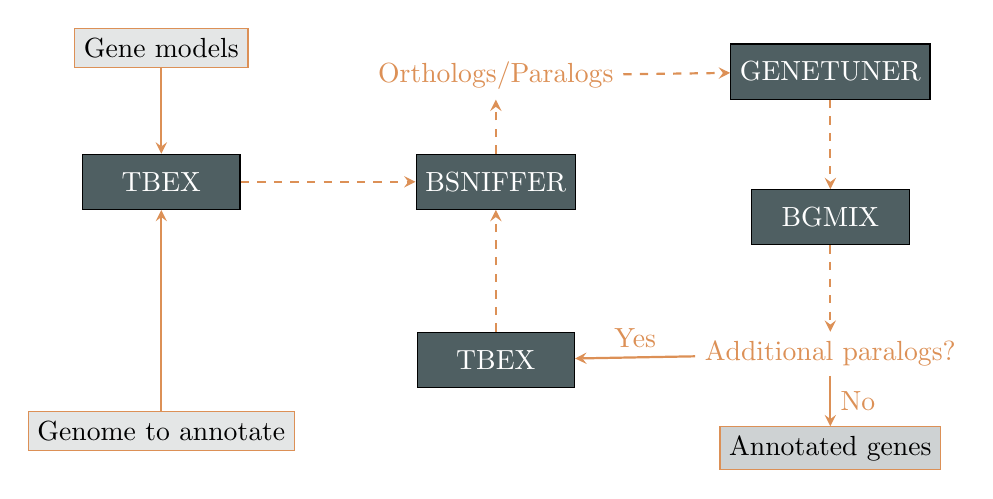
\begin{tikzpicture}[align=center,node distance=2cm]
	\node (b)[]{};
	\node (a)[left=4cm of b]{};
	\node (c)[right=4cm of b]{};
	\node (tbex)[software, above=1.2cm of a]{TBEX};
	\node (bsniffer)[software, above=1.2cm of b]{BSNIFFER};
	\node (genetuner)[software, above=2.6cm of c]{GENETUNER};
	\node (bgmix)[software, above=0.75cm of c]{BGMIX};
	\node (tbex2)[software, below=0.1cm of b]{TBEX};
	\node (genes)[input, above=3cm of a]{Gene models};
	\node (genome)[input, below=1.1cm of a]{Genome to annotate};
	\node (orpar)[midput, above=2.6cm of b]{Orthologs/Paralogs};
	\node (add)[midput, below=0.1cm of c]{Additional paralogs?};
	\node (anno)[output, below=1.3cm of c]{Annotated genes};
	\draw [flow] (tbex) -- (bsniffer);
	\draw [flow] (bsniffer) -- (orpar);
	\draw [flow] (orpar) -- (genetuner);
	\draw [flow] (genetuner) -- (bgmix);
	\draw [flow] (bgmix) -- (add);
	\draw [flow] (tbex2) -- (bsniffer);
	\draw [inout] (genes) -- (tbex);
	\draw [inout] (genome) -- (tbex);
	\draw [inout] (add) -- node [above] {Yes} (tbex2);
	\draw [inout] (add) -- node [right] {No} (anno);
	\end{tikzpicture}
	\caption[Information flux in the execution process of BATI]{\footnotesize Information flux in the execution process of BATI.}
	\label{f_bati_flow}
\end{figure}

The program \texttt{bsniffer} generates a file per gene in which the results are reorganized in a more readable way.
Additionally, the script calculates a score based on how complete, large and good match a hit is.
Considering all of this, one can choose the best combination of hits, only being restricted by the contigs and not by the \texttt{tblasn} combinations.
The program will also mark the hits that have already been used in building a gene to prevent their reuse.
Once the best choice has been made, a predicted model is created and the next gene can be analysed in the same way.

The step run by \texttt{genetuner} provides a graphical interface that allows the user to move around the annotated exons of the gene, and shows the genome to be annotated and its three translated frames in the chosen strand.
Besides the clearly distinguishable sequences of exons and introns, if the cDNA for the model genes was provided, this will also be available to double-check similarities.
The aim of this step is to use the interactive view of the chosen alignment and to polish it as much as possible.
This can be accomplished by correcting the exon-intron junctions, adding or deleting exons, or even splitting or mixing different exons (usually because of a \emph{frameshift}).
Some of these cases may be tackled by paying attention to the conserved splicing points, but in many other cases it may be helpful to check external information sources such as published works regarding a specific gene, different databases, or related (and already annotated) organisms.
This step is crucial, as it allows users to improve the annotation in ways that are not accessible during automatic annotation. The program also allows users to note down comments on particular regions. This is very important, since a wrong exon-intron union may be later interpreted as a spurious mutation.
The graphical interactive interface includes several ways to move around, and several way to edit the current selection.
Additionally, it allows the writing of warning when needed and the ability to increase or decrease sensitivity locally, as well as to perform different kinds of searches.
This is the step where the researcher experience is most valuable.

\texttt{bgmix} summarizes all the hits in one file, indicating to which model protein each hit is more similar, and also if it has been used to build a gene already.
Because of its usefulness, it is usually run twice, first after the \texttt{tbex} step, to have a general idea of the best match to each hit, and once everything is annotated, to check for unused hits, since those can build up a whole gene which can be a duplication or even a new one.
If this is the case, the protocol is to duplicate the protein sequence file (and, if available, the cDNA) of the duplicated gene, and re-run the whole pipeline.
Once this result of \texttt{bgmix} has no more obvious hits, we can consider the set of genes of interest annotated.

By using the data sets mentioned in subsection \ref{ss_matmet_molecular_gene_selection} the whole annotation process, including the pertinent comparisons and the final validation using Sanger is summarized in figure \ref{f_annotation_process}.

\begin{figure}[t]
	\centering
	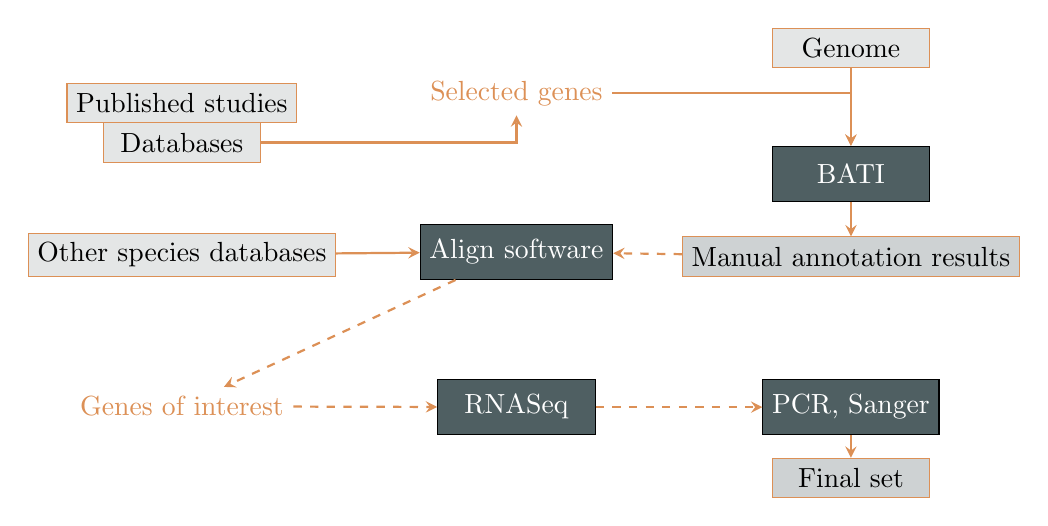
\begin{tikzpicture}[align=center,node distance=2cm]
	\node (b)[]{};
	\node (a)[left=4cm of b]{};
	\node (c)[right=4cm of b]{};
	\node (pub) [input, above=2cm of a] {Published studies};
	\node (db) [input, above=1.5cm of a] {Databases};
	\node (cherry) [midput, above=2.1cm of b] {Selected genes};
	\node (genome) [input, above=2.7cm of c] {Genome};
	\node (bati) [software, above=1cm of c] {BATI};
	\node (results) [output, above=0.05cm of c] {Manual annotation results};
	\node (db2) [input, above=0.05cm of a] {Other species databases};
	\node (comp) [software, above=0.01cm of b] {Align software};
	\node (int) [midput, below=1.1cm of a] {Genes of interest};
	\node (pcr) [software, below=1cm of c] {PCR, Sanger};
	\node (rna) [software, below=1cm of b] {RNASeq};
	\node (final) [output, below=2cm of c] {Final set};
	\draw [inout] (db) -| (cherry);
	\draw [inout] (cherry) -| (bati);
	\draw [inout] (genome) -- (bati);
	\draw [inout] (bati) -- (results);
	\draw [inout] (db2) -- (comp);
	\draw [flow] (results) -- (comp);
	\draw [flow] (comp) -- (int);
	\draw [flow] (int) -- (rna);
	\draw [flow] (rna) -- (pcr);
	\draw [inout] (pcr) -- (final);
	\end{tikzpicture}
	\caption[Complete manual annotation process]{\footnotesize Complete manual annotation process, including all the steps for the initial data to the final selection of corroborated genes of interest.}
	\label{f_annotation_process}
\end{figure}

When manually annotating a genome, especially in the case of \textit{de novo} genomes, one must consider that some of the results may be artefacts produced by the \textit{de novo} assembly.
There are multiple causes for this error to appear, \textit{e.g.} absence or reduced coverage of a specific regions of the genome leading us to think that genes may have been lost, or a lot of heterozygous positions concentrated in a region, which may provoke the assembler to assume that they are different regions, hence misidentifying a duplication.
For this reason, hypotheses that arise from annotations must always be corroborated by other studies in order to be fully reliable.
Some of these additional tests can range from checking the quality of the specific region we are interested on, or studying RNA-Seq data (if available), to performing PCR amplification and Sanger sequencing of the interesting region. 

\subsection{Expansion of gene families} \label{ss_matmet_bioinformatics_expansion}

We performed several pairwise alignments of the predicted proteins from the automatic annotation to the UniProt \cite{Bateman2019} databases of human and \textit{P. sinensis} proteins using BLAST (v2.6.011) \cite{Altschul1990}.
Using in-house perl scripts (available in a public repository (\href{https://github.com/vqf/LG}{https://github.com/vqf/LG}), we grouped these sequences into one-to-one, one-to-many, and many-to-many orthologous relationships.
Only alignments with a coverage of at least 80\% of the longer protein, and with more than 60\% of identity were considered for the analysis.
Finally, we searched for family expansions specifically present in \textit{C. abingdonii}, by examining the aforementioned groups of orthologs.
The results were manually curated.
This way, we constructed extended orthology sets that may contain more than one sequence per species.

\subsection{Positive selection} \label{ss_matmet_bioinformatics_positive_selection}

To search for signatures of selection affecting the predicted set of genes, we used BLAST and in-house perl scripts to pairwise align all available protein sequences from human (\textit{H. sapiens}), mouse (\textit{M. musculus}), dog (\textit{Canis lupus familiaris}), gecko (\textit{Gekko japonicus}), green anole lizard (\textit{A. carolinensis}), python snake (\textit{Python bivittatus}), common garter snake (\textit{Thamnophis sirtalis}), Habu viper (\textit{Trimeresurus mucrosquamatus}), budgerigar (\textit{Melopsittacus undulatus}), zebra finch (\textit{Taeniopygia guttata}), flycatcher (\textit{Ficedula albicollis}), duck (\textit{Anas platyrhynchos}), turkey (\textit{Meleagris gallopavo}), chicken (\textit{G. gallus}), Chinese softshell turtle (\textit{P. sinensis}), green sea turtle (\textit{C. mydas}) and painted turtle (\textit{C. p. bellii}).
We focused only on those genes with a one-to-one ortholog status in every species, and missing in no more than 3 species (excluding \textit{C. abingdonii}), as described in previous studies \cite{Keane2015}.
We then aligned each group separately with PRANK v.150803 using the codon model and analysed the alignments with \texttt{codeml} from the PAML package \cite{Yang2007}.

To search for genes with signatures of positive selection affecting \textit{C. abingdonii} genes specifically, we executed two different branch models, M0, with a single $\omega$0 value (where $\omega$ represents the ratio of non-synonymous to synonymous substitutions) for all the branches (nested), and M2a, with a foreground $\omega$2 value exclusive for \textit{C. abingdonii} and a background $\omega$1 value for all the other branches.
Genes with a high $\omega$2 value ($>$1) and a low $\omega$1 value ($\omega$1$<$0.2 and $\omega$1$\approx\omega$0) in \textit{C. abingdonii}, but not in \textit{P. sinensis} (Table \ref{app_t_positive_selection}) were then considered as candidates to be under positive selection.
As a control, M2a was repeated using \textit{P. sinensis} as the foreground branch, and no overlapping genes were found in the result.
Then, we used the M8 branch model to assess the individual importance of every site in these positively selected genes, obtaining a list of sites possibly under selection.
The equivalent sites were examined in the Aldabra tortoise through alignments, to evaluate which of these important residues were altered (Table \ref{app_t_site_positive_selection}).

\section{Code development}

\subsection{Database management CGI} \label{ss_matmet_code_cgi}

The different scripts, coded in Perl (version > 5.20), and using a CGI\nomenclature{CGI}{Common Gateway Interface} protocol for executing them via web requests, orchestrate the interaction with the user, the creation/edition of the database, and the editing/creating of the final HTML\nomenclature{HTML}{HyperText Markup Language} that will display the website. % (for examples on this set of scripts, check appendix \ref{s_database_management}).
In parallel, a couple of simple HTML files create the UI%\nomenclature{UI}{User Interface} 
for the editing of the database and the CGI request for the main set of programs.
Briefly, the steps of the process would be as follow:

\begin{enumerate}[topsep=1ex,itemsep=-1ex]
	\item A JSON\nomenclature{JSON}{JavaScrip Object Notation}-build database, containing all the information about the degradome, degradomopathies, protease family, and information related to our laboratory (\textit{e.g.} members, news, software, ...) is taken as input by one script. This JSON is then displayed as a interactive HTML-coded table.
	\item In this table one can made editions, additions or even deletions. For each of these modifications, there is an appropriate button to execute the pertinent script and perform the desired change.
	\item The invoked script then creates a copy of the database as it is (to be kept as a security copy), then applies the required changes to the database, and finally calls for the last script.
	\item This will take the new altered database as an input and build the different parts of the website taking into consideration the changes everywhere (\textit{e.g.} if you add a protease, every line that mentions the number of proteases will change so that the number displayed is increased by 1).
	\item Ideally, the user that made the modification should now check that everything is in order, since by repeating this process with a new modification will overwrite the saved copy. Ultimately, if even after checking some mistake is spotted and it is too late to recover the data not all will be lost, since an automatic process in the server keeps weekly security copies.
\end{enumerate}

It is noteworthy that regular queries to the website work in a similar way as step 4, since the information in the JSON file is queried using the AJAX\nomenclature{AJAX}{Asynchronous JavaScript And XML} technology through jQuery, hence being dynamically fetched by request. If the browser lacks JavaScript or if this is disabled, the website will redirect the user to a static table with all the information.

\subsubsection*{Website Public Interface}

The website is built using responsive-by-design technology, which allows the browser to \quotes{rearrange} the different HTML-containers in order to adapt it to the available display.
Also, by interacting with the displayed information, the user may ask for more details of specific parts.
By requesting this information interactively and using the aforementioned technologies waiting times for the loading of the different tables is reduced.
%Examples of this UI, including those regarding its responsiveness to different displays, and the pop-up-delivered information, can be found in the appendix \ref{a_figures}, figures \ref{fig_bootstrap} and \ref{fig_pop-up}.

% Victor me ha parecido más razonable no incluir capturas de pantalla ni trozos de codigo como tal, no me prece que quede muy profesional... Respecto a las imagenes igual se pueden poner en la presentación pero en el texto impreso me parece demasiado, no? Que opinas?


\chapter{Results}

\section{Sperm whale degradome} \label{s_sperm_whale_results}

We have annotated the complete set of proteases (or degradome) of the sperm whale using human proteins as model sequences, and we have performed several comparisons between them and those of other cetaceans and human.
Overall, most of the predicted losses and gains of protease genes mirror those already described in minke \cite{Yim2014c} and bowhead whales \cite{Keane2015}.
Nevertheless, several events stand out as independent or specific, providing interesting hypotheses about the evolution of sperm whales in the context of cetacean evolutionary history (Figure \ref{f_results_sperm_whale_summary}).
In addition to the usual selective pressure on the immune and reproductive system of mammals, the unique aquatic environment of cetaceans has prompted numerous changes affecting protease genes involved in blood homoeostasis, digestion and skin maintenance.

\subsection{Immunity and inflammation} \label{ss_sperm_whale_results_immuno}

In the context of immunology, we have found a conserved premature stop codon at the coding sequence of cetacean \textit{MMP12}.
Interestingly, besides the conserved premature stop codon (in {p.W109}), sperm whale present an additional, specific one in {p.G93} (figure \ref{f_results_sperm_whale_alignments_inmuno}).
This metalloprotease is preferentially expressed in macrophages, where it can modulate inflammatory responses.
Its role is essential in multiple pathological settings, including lung emphysema \cite{Ishii2014} and atherosclerotic disease \cite{Proietta2014}.
Notably, the loss of expression of \textit{MMP12} in lung adenocarcinoma cells inhibits their growth and invasion capacities \cite{Lv2015}.
%These precedents suggest that the loss of \textit{MMP12} occurred early during the evolution of cetaceans, and might be related to the adaptation of the immune and vascular systems to an aquatic environment.
%The pro-tumorigenic activity of MMP12 also suggests that this event might be important to decrease the probability of developing cancer as the body size of cetaceans increased.
Similarly, \textit{TPSAB1}, one of the major proteases present in mast cells, has been inactivated in all analysed cetaceans via conserved premature stop codon in {p.D276} (figure \ref{f_results_sperm_whale_alignments_inmuno}).
Additional premature stop codons, both of them independently arisen, can be found in the sequences of sperm whale and minke whale, but they appear in non-conserved areas of the gene.
This protease is secreted in the response to degranulation, and has been implicated as a mediator in the pathogenesis of asthma and other allergic disorders \cite{Abdelmotelb2014}.
%This loss also suggests a lower inflammatory potential in sperm whales.
%The fact that other cetaceans have independently lost this gene suggests that this moderation in the inflammatory response may be a trend throughout the evolution of these organisms.

In addition, we have found that \textit{CASP12}, a modulator of the activity of inflammatory caspases, presents several premature stop codons as a result of a shared frameshift (starting in {p.L101} and is likely a pseudogene (Figure \ref{f_results_sperm_whale_alignments_inmuno}; \cite{McIlwain2015}).
The annotations of this gene in the other cetaceans, suggests a complex evolutionary history. 
Specifically, Delphinoideos and Physeteroideos seem to share the same frameshift (starting in {p.L30}) which must have arisen via convergent evolution, since their closer relatives Monodontiddeos lack this alteration.
Similarly, a different position presents another premature stop codon ({p.R221*}), shared among all cetacea but Delphinoidea (Figure \ref{app_f_casp12_align}).
%This suggests that the loss of \textit{CASP12} is also an early event in the evolution of cetaceans.
While this caspase is conserved and functional in most terrestrial mammals, it is lost in most humans through a different mechanism involving the loss of the canonical stop codon.
It has been shown that human displaying this protease in its active form are more sensitive to infection and sepsis \cite{Saleh2004}.
%Therefore, this event seems to provide an interesting case of convergent evolution between humans and cetaceans, suggesting that similar adaptations may benefit organisms living in very different environments.
%A similar situation has likely shaped the evolution of \textit{PRSS33}, a macrophage-specific serine-protease.
%Thus, the ortholog present in sperm whale shares a conserved stop codon with other cetaceans, whereas several primates have lost \textit{PRSS33} through different mechanisms \cite{Puente2005,Johnson2006,Locke2011}.
% He quitado la parte relativa a PRSS33 por que no soy capaz de encontrar a que me refería... Si te parece cuando termine lo comentamos por si tu recuerdas algo más.

\begin{figure}[t!]
    \begin{center}
        \includegraphics[width=\textwidth]{figures/alignment_immune.pdf}
        \caption[Alignments of proteases related to immunology in cetaceans]{\footnotesize Alignments of proteases related to immunology in cetaceans. Arrows mark the positions mentioned in the text, and the different intensity of colour reflects the degree of conservation within the alignment. \hsap; \bacu; \bmys; \mmon; \dleu; \ttru; \oorc; and \pmac.}
        \label{f_results_sperm_whale_alignments_inmuno}
    \end{center}
\end{figure}

Finally, we have found interesting hallmarks of the evolutionary history of \textit{MASP2} in cetaceans.
This serine protease binds specific carbohydrates in the surface of invading microorganisms and activates the alternative complement pathway of innate immunity.
Thus, MASP2 cleaves factors C4 and C2 to initiate the proteolytic cascade that leads to the formation of the membrane-attack complex.
Consistent with this important role, a missense mutation in humans MASP2 (D105G), which abolishes its activity, correlates with severe immunological deficiencies \cite{Stengaard-Pedersen2003}.
However, the genome of the sperm whale shows a truncated version of this important gene because of a premature stop codon, which is upheld by the RNA-Seq analysis.
This truncated ortholog also features a specific D105A change.
%Notably, among the additional cetaceans we have studied, only killer whales feature a truncated version of \textit{MASP2}, and the predicted coding sequence shares no conserved stop codons with the ortholog in sperm whales.
%In sperm whales, this loss may have occurred through a stepwise mechanism, first with a missense mutation, reminiscent of a disease-related variant, and then with a nonsense mutation.
%This kind of predicted pathogenic deviations may play a very important role during speciation, as shown by Bateson, Dobzhansky and Muller \cite{Orr1996,Kondrashov2002}.
%Intriguingly, both truncated proteins are expected to contain lectin-binding domains, but not the serine-protease domain, which suggests a possible compensating mechanism through binding of a different protease to these domains.
Interestingly, dolphins also display a truncated version of this protein, in this case caused by a premature stop codon resulting from a frameshift at {p.G454}, again suggesting convergent evolution (Figure, \ref{app_f_masp12_align}).
Therefore, these data suggest that \textit{MASP2} has been independently lost in at least two Odontoceti, but is present and functional in killer whales.
Further studies will be necessary to identify the putative compensatory mutations that permit the loss of \textit{MASP2} without any obvious disadvantage in certain odontocetes. 

\subsection{Coagulation and blood pressure} \label{ss_sperm_whale_results_blood}

%One of the most conspicuous traits of the aquatic environment is the hydrostatic pressure and lack of net weight experienced by cetaceans.
%This, in turn, must prompt compensatory mechanisms in the control of blood pressure and coagulation to avoid haemostatic accidents.
We have confirmed the lack of both \textit{F12} and \textit{KLKB1}, two serine proteases which participate in the kinin-kallikrein system \cite{Irmscher2018}.
According to our annotation, \textit{F12} was lost in a common ancestor to all cetaceans, presenting 2 conserved premature stop codons ({p.Y391*} and {p.E521*}).
An alignment of the annotated sequences also shows evidence of more recent events, like an additional premature stop codon shared by all non-Physeteroideos Odontoceti in {p.E514*}, an additional premature stop codon shared by Delphinoideos in {p.W406*} (Figures \ref{f_results_sperm_whale_alignments_blood}, and \ref{app_f_f12_align}).
On the other hand, \textit{KLKB1}, seems to be in different states of pseudogenization in Misticeti and appears to be completely absent in some Odontoceti.
However, it must be noted that complete gene losses can be mimicked by assembly artefacts.
The kinin-kallikrein system is important in inflammation, blood pressure control, coagulation and pain \cite{Verweij2013a}.
%In fact, a genome association analysis with human populations has uncovered variants of these serine proteases putatively related to increased levels of vasoactive peptides.\cite{Verweij2013a}.

\begin{figure}[t!]
    \begin{center}
        \includegraphics[width=\textwidth]{figures/alignment_blood.pdf}
        \caption[Alignments of proteases related to blood homoeostasis in cetaceans]{\footnotesize Alignments of proteases related to blood homoeostasis (and coagulation) in cetaceans. Arrows mark the positions mentioned in the text, and the different intensity of colour reflects the degree of conservation within the alignment. \hsap; \bacu; \bmys; \mmon; \dleu; \ttru; \oorc; and \pmac.} 
        \label{f_results_sperm_whale_alignments_blood}
    \end{center}
\end{figure}

Furthermore, the related serine proteases \textit{F7}, \textit{TMPRSS11F} and \textit{TMPRSS11B} have been shown to constitute targets of selection in Mysticeti, probably related to their role in coagulation \cite{Keane2015}.
In our data set, \textit{F7} appears to be a functional gene in sperm whales, whereas both \textit{TMPRSS11F} and \textit{TMPRSS11B} have been lost through premature stop codons.
%Notably, both \textit{TMPRSS11B} and \textit{TMPRSS11F} were apparently lost in an independent event, which again reinforces the role of coagulation modulation in cetaceans.
Specifically, \textit{TMPRSS11B} seems to be in different states of pseudogenization in the analysed cetaceans.
It presents a common premature stop codon shared by all Delphinoidea ({p.R402*}), whereas in sperm, bowhead, and Minke whales a different point mutation has caused the gain of a premature, non-conserved stop codon (Figures \ref{f_results_sperm_whale_alignments_blood}, and \ref{app_f_tmprss11b_align}).
\textit{TMPRSS11F}, on the other hand, presents a frameshift (starting in {p.R411}), conserved in all cetaceans, which causes several premature stop codons (Figure \ref{f_results_sperm_whale_alignments_blood}).

% AMZ2 es uno de los papers afectados por la retractación de los papers de JBC... Lo dejo comentado...
%Possibly related to these events is the selective loss of \textit{AMZ2} in sperm whales.
%This zinc metalloprotease has been hypothesized to cleave angiotensin, and therefore it might play an important role in blood pressure homoeostasis \cite{}.
%The loss-of-function for this gene is predicted on the basis of a premature stop codon located at the catalytic site of its proteolytic domain.
% DPEP2 es dudosa... Las lecturas que soportan el codón de parada tienen otras variantes. Hay otro codón de parada del que no tengo secuencias crudas.
%Finally, \textit{DPEP2} and \textit{DPEP3}, two members of the membrane dipeptidase family (M19) seem to have been lost in sperm whales specifically.
%These peptidases, also known as MBD-2 and MBD-3 are expressed in several tissues, including kidney, and can cleave and inactivate leukotriene D418.
%Therefore, blood homoeostasis in sperm whales seems to feature different regulation levels compared to other cetaceans.
%Comparison with other deep-swimming whales may offer clues as to whether these changes are related with the diving abilities of this organism.

%Together, these changes suggest that the mammalian potential for clotting and blood pressure are excessive in an aquatic environment, and these systems had to be modulated through the loss of proteases implicated in related proteolytic cascades.

\subsection{Skin homoeostasis} \label{ss_sperm_whale_results_skin}

%Living underwater also sets the skin of mammals as a target of evolutionary pressure.
%Several events in the degradome of cetaceans might be related to this adaptative process.
The cysteine-protease \textit{CAPN12} has been lost through different, non-overlapping premature stop codons and frameshifts in sperm whale, dolphin, and bowhead and minke whales.
In the case of the sperm whale specifically, the truncation is produced by one frameshift starting at {p.F131} (Figure \ref{f_results_sperm_whale_alignments_skin}).
This protease is preferentially expressed at the cortex of the hair follicle \cite{Dear2000}.
%The loss of \textit{CAPN12} might be related to the lack of hair in most of the cetacean body.

\begin{figure}[t!]
    \begin{center}
        \includegraphics[width=\textwidth]{figures/alignment_skin.pdf}
        \caption[Alignments of proteases related to skin homoeostasis in cetaceans]{\footnotesize Alignments of proteases related to skin homoeostasis in cetaceans. Arrows mark the positions mentioned in the text, and the different intensity of colour reflects the degree of conservation within the alignment. \hsap; \bacu; \bmys; \mmon; \dleu; \ttru; \oorc; and \pmac.}
        \label{f_results_sperm_whale_alignments_skin}
    \end{center}
\end{figure}

Likewise, the serine-protease KLK8 appears to be absent in all analysed cetaceans, except for sperm whales, through two different mechanisms, each specific to one parvorder.
While mysticetes share a common premature stop codon at {p.88}, Delphinoidea displays a different premature stop codon at {p.170}.
In sperm whales, this KLK8 displays a complete open-reading frame, but its catalytic site is mutated (starting at {p.G255A}) to a theoretically inactive form (Figure \ref{f_results_sperm_whale_alignments_skin}).
Therefore, sperm whale's \textit{KLK8} is expected to be a functional gene producing a non-functional protease.
Nevertheless, inactive proteases can be important, since they can still bind and sequester substrates.

Finally, another kallikrein, \textit{KLK7}, seems to have been specifically lost in a common ancestor of mysticetes, but not in the odontocetes analysed (including sperm whales).
Both \textit{KLK7} and \textit{KLK8} have been related to skin homoeostasis \cite{Kishibe2007}, and some experiments suggest that \textit{KLK8} might be directly involved in the terminal differentiation and desquamation of the \emph{stratum corneum}, the utmost layer of the skin in mammals \cite{Kuwae2002}.
%This complex pattern of convergent evolution suggests that skin-related proteases have played important roles in aquatic adaptation, in a process possibly influenced by the specific and somewhat contradictory requirements of heat insulation, buoyancy and deep diving.

\subsection{Digestive system} \label{ss_sperm_whale_results_digestive}

%Cetaceans also feature diverse feeding strategies, based on krill (Mysticeti) or fish, squids and crustaceans (Odontoceti).
The evolution of the digestive system of these mammals has included the loss of several metallocarboxypeptidases from the M14 family.
Thus, \textit{CPA2}, \textit{CPA3} and \textit{CPO} were lost in all cetaceans examined.
Surprisingly, \textit{CPA3} may have been lost independently in sperm whales and in an ancestor of baleen whales. % Figure?
Dolphin \textit{CPA3} also features an independent premature stop codon.
Furthermore, sperm-whale \textit{CPB1}, also from the M14 family, features two premature stop codons not present in Mysticeti. % Where?
Notably, those stop codons are not present in the corresponding ortholog from dolphins.
As expected, odontocetes retain functional orthologs of \textit{KLK4} and \textit{MMP20}, two proteases involved in dentition which are lost in mysticetes \cite{Keane2015}.

%These results suggest that protease gene losses have been important in the evolution of the digestive system of cetaceans.
%At least in some cases, the genetic causes for these losses have been independent even between Odontocetis.
%This case of convergent evolution suggests that those events were highly favoured at the trophic level where cetaceans thrive.

\subsection{Sperm whale-specific traits} \label{ss_sperm_whale_results_specific}

Several important events in the sperm-whale degradome seem to be specific for this mammal, and probably merit further study.
Thus, \textit{MMP7} (matrilysin-1), a metalloprotease with the ability to cleave scaffolding proteins in the extracellular matrix, contains a premature stop codon ({p.W149*}) in sperm-whales (figure \ref{f_results_sperm_whale_alignments_mmp7}) \cite{Grindel2018}.
The second member of the matrilysin sub-family, \textit{MMP26} or \textit{matrilysin-2}, is primate-specific \cite{Uria2000}.
If confirmed, this would be the first case of spontaneous lack of matrilysins in a mammalian species.
%The \textit{MMP} family has a large number of members with partially overlapping functions, and therefore the loss of one protease can be overcome by the activity of other paralogs.
%However, mice deficient in \textit{MMP7} have been shown to respond differently to challenges like re-epithelialization \cite{Swee2008}.
%Interestingly, high levels of expression of this metalloprotease have also been shown to promote metastasis \cite{Li2014a,Koskensalo2011}, which suggests a putative sperm whale-specific mechanism to counteract the problems underlined in Peto’s paradox.

\begin{figure}[b!]
    \begin{center}
        \includegraphics[width=\textwidth]{figures/alignment_mmp7.pdf}
        \caption[Alignment of protease MMP7 in cetaceans]{\footnotesize Alignment of protease MMP7 in cetaceans. The arrows marks positions mentioned in the text. \hsap; \bacu; \bmys; \mmon; \dleu; \ttru; \oorc; and \hsap.}
        \label{f_results_sperm_whale_alignments_mmp7}
    \end{center}
\end{figure}

Finally, the cysteine-protease \textit{CASP3} has been specifically duplicated in sperm whales in a retrotranscription-involving event (Figure \ref{f_results_sperm_whale_alignments_casp3}).
The resulting single-exon duplicate contains a complete, uninterrupted open reading frame and features few amino acid changes compared to the original form.
This protease is involved in one of the proteolytic cascades leading to apoptosis \cite{McIlwain2015}.
In addition to its putative role in cancer progression, \textit{CASP3} has also been involved in brain physiology as the predominant caspase that cleaves amyloid-beta 4A precursor protein.

\begin{figure}[b!]
    \begin{center}
        \includegraphics[width=\textwidth]{figures/alignment_casp3.pdf}
        \caption[Alignment of protease CASP3 in cetaceans]{Alignment of protease CASP3 in cetaceans, including the sequence of sperm whale's specific duplication. \hsap; \bacu; \bmys; \mmon; \dleu; \ttru; \oorc; and \pmac.}
        \label{f_results_sperm_whale_alignments_casp3}
    \end{center}
\end{figure}

\section{Gal\'{a}pagos giant tortoise genome analysis} \label{s_george_genome_results}

\subsection{Genome assembly} \label{ss_george_genome_results_assembly}

We used Illumina paired reads, mate pairs and PacBio reads to assemble the genome of Lonesome George in 10,623 scaffolds with an N50 of 1.27 Mb, with the largest scaffold being longer than 10 Mb (Table \ref{t_george_statistics}).

\begin{table}[h]
    \centering
    \caption[\textit{C. abingdonii} genome statistics]{\footnotesize \textit{C. abingdonii} genome statistics.}
    \begin{tabular}{lrrr}
        %\cline{2-4}
        \hline \hline
        & \multicolumn{1}{c}{Scaffolds with GAPS} & \multicolumn{1}{c}{Scaffolds without GAPs} & \multicolumn{1}{c}{Contigs with Ns} \\ \hline \hline
        \multicolumn{1}{l}{Seqs}          & 10,623            & 10,623            & 10,623 \\
        \multicolumn{1}{l}{Min}           & 886 bp            & 886 bp            & 130 bp \\
        \multicolumn{1}{l}{Median}        & 6,499 bp          & 4,304 bp          & 16,213 bp \\
        \multicolumn{1}{l}{Mean}          & 216,581 bp        & 204,233 bp        & 33,555 bp \\
        \multicolumn{1}{l}{Max}           & 10,495,589 bp     & 10,223,643 bp     & 1,220,627 bp \\ \hline
        \multicolumn{1}{l}{Total}         & 2,300,749,194 bp  & 2,169,570,871 bp  & 2,169,570,871 bp \\
        \multicolumn{1}{l}{N50}           & 1,277,207 bp      & 1,227,724 bp      & 74,527 bp \\
        \multicolumn{1}{l}{N90}           & 337,476 bp        & 331,274 bp        & 18,547 bp \\
        \multicolumn{1}{l}{N95}           & 174,219 bp        & 172,536 bp        & 10,818 bp \\ \hline
        \multicolumn{1}{l}{Non-gapped Ns} & \multicolumn{3}{c}{23,455 bp} \\ \hline \hline
    \end{tabular}
    \label{t_george_statistics}
\end{table}

The final assembly (\emph{CheloAbing 1.0}) is 2.3 Gb long, a size consistent with other turtle assemblies such as \textit{C. p. bellii} (2.59 Gb) \cite{BradleyShaffer2013}, and {\textit{C. mydasa}} and \textit{P. sinensis} (both around 2.2 Gb) \cite{Wang2013b}.

According to the masking procedure, 28.5\% of the genome represents repetitive elements.
Of these, the larger group is that of retroelements, which add up to 17.86\% of the assembly (Table \ref{t_george_repeatmasker}).

\begin{table}[h]
    \centering
    \caption[Repeated elements in \textit{C. abingdonii}]{\footnotesize Repeated elements in the genomes of \textit{C. abingdonii} and \textit{C. p. bellii}, showing number of elements (\texttt{n}), total length (\texttt{bp}), and percentage of genome covered (\texttt{\%}).}
    \begin{tabular}{lrrrrrrr}
        %\cline{2-6}
        \hline \hline
        & & \multicolumn{3}{c}{\textit{C. abingdonii}} & & \multicolumn{2}{c}{\textit{C. p. bellii}} \\
        \cline{3-5} \cline{7-8}
        \multicolumn{1}{l}{Repeat type}       & & n         & bp            & \%            & & bp            & \% \\ \hline \hline
        \multicolumn{1}{l}{SINEs}             & & 215,691   & 33,047,802    & 1.40          & & 44,277,662    & 1.87 \\
        \multicolumn{1}{l}{PLEs}              & & 156,168   & 35,941,354    & 1.56          & & -             & - \\
        \multicolumn{1}{l}{LINEs}             & & 572,190   & 231,609,979   & 10.07         & & 248,848,977   & 10.52 \\
        \multicolumn{1}{l}{LRTs}              & & 243,123   & 146,157,459   & 6.35          & & 123,030,173   & 5.20 \\
        \multicolumn{1}{l}{DNA Transposons}   & & 1,044,675 & 227,423,152   & 9.88          & & 18,952,044    & 9.80 \\ 
        \multicolumn{1}{l}{Unclassified}      & & 84,016    & 17,050,133    & 0.74          & & 20,076,666    & 0.80 \\ 
        \multicolumn{1}{l}{Small RNAs}        & & 42,858    & 8,412,400     & 0.37          & & 8,527,612     & 0.36 \\
        \multicolumn{1}{l}{Simple repeats}    & & 8,199     & 1,475,310     & 0.06          & & 11,395,517    & 0.48 \\
        \multicolumn{1}{l}{Low complexity}    & & 192       & 64,291        & $\sim$0.00    & & 2,244,030     & 0.09 \\ \hline \hline
    \end{tabular}
    \label{t_george_repeatmasker}
\end{table}

Additionally, since PacBio sequencing features frequent errors, we compiled regions covered only by these reads and added them to the header of the assembly.
A file containing this information is available in the assembly entry at the NCBI database (\href{https://www.ncbi.nlm.nih.gov/nuccore/PKMU00000000.1/}{www.ncbi.nlm.nih.gov/nuccore/PKMU00000000.1/}).
Point variants belonging to these regions are not reported unless validated by other means.

In parallel, we assessed the suitability of \emph{CheloAbing 1.0} for gene annotation.
From this analysis, we located 96.4\% of the common core of conserved genes, out of which 0.6\% were duplicated genes.
While the percentage of fragmented genes (5.7\%) was relatively high, these results are compatible with a moderately good quality of assembly, with only 1.9\% totally missing.
In other species considered for comparison, the percentage of missing genes was always higher, while maintaining a similar completeness percentage (Table \ref{t_george_busco}).

\begin{table}[h]
    \centering
    \caption[Comparative BUSCO analysis of \textit{C. abingdonii}]{\footnotesize Comparative BUSCO analysis of \textit{C. abingdonii}, published data from \textit{G. agassizii}, and \textit{de novo} analysis of \textit{H. sapiens} (CH38).}
    \begin{tabular}{lrrrrrrrrr}
        %\cline{2-7}
        \hline \hline
        & & \multicolumn{2}{c}{\textit{C. abingdonii}} & & \multicolumn{2}{c}{\textit{G. agassizii}} & & \multicolumn{2}{c}{\textit{H. sapiens} (CH38)} \\
        \cline{3-4} \cline{6-7} \cline{9-10}
        & & n & \% & & n & \% & & n & \% \\ \hline \hline
        \multicolumn{1}{l}{Completed}    & & 2,391 & 92.4  & & 2,387 & 92.4  & & 2,355 & 91.1 \\
        \multicolumn{1}{l}{Duplicated}   & & 16    & 0.6   & & 22    & 0.9   & & 72    & 2.8 \\
        \multicolumn{1}{l}{Fragmented}   & & 147   & 5.7   & & 138   & 5.3   & & 112   & 4.3 \\
        \multicolumn{1}{l}{Missing}      & & 48    & 1.9   & & 61    & 2.3   & & 119   & 4.6 \\ \hline
        \multicolumn{1}{l}{Total}        & & 2,586 & 100   & & 3,023 & 100   & & 2,586 & 100 \\ \hline \hline
    \end{tabular}
    \label{t_george_busco}
\end{table}

\subsection{Automatic annotation of \emph{CheloAbing 1.0}} \label{ss_results_george_automatic_annotation}

As a result of the automated annotation process, we obtained 27,208 predicted genes with putative functions assigned. 
A multifasta file containing all protein sequences is available in a public repository (\href{https://github.com/vqf/LG}{https://github.com/vqf/LG}).

With these data, we constructed extended orthology sets that may contain more than one sequence per species.
These orthology sets capture most of the known protein families, although some of these families appear split according to sequence similarity.
Almost all of these splits occur both in the human-to-\textit{P. sinensis} and in the {human-to-\textit{C. abingdonii}} comparisons.
Since assembly errors may mimic gene losses, we decided to only test these sets for {\textit{C. abingdonii}-specific} expansions.
The interrogation of these sets suggests the existence of several high copy-number gene families in tortoises and turtles but absent in humans.
Most of these families show homology to viral retrotranscriptases, consistent with the hypothesized expansion of CR1 retrotransposons in ancestral amniotes followed by dominance of L1 LINEs in therians \cite{Suh2014}.
After manual curation of the results, we found 12 examples of gene families displaying extra copies in \textit{C. abingdonii} compared to turtles (Table \ref{t_george_expansions}).
Each of those genes was also identified from the aligned reads in the Aldabra giant tortoise genome, and 10 of these amplifications were also identified in the genome of Agassiz’s desert giant tortoise \cite{Tollis2017}.
Interestingly, a functional annotation clustering analysis of these 12 genes found a significant enrichment in the \quotes{extracellular exosome} GO category (8 genes; \textit{ATP6V1A}, \textit{EEF1A1}, \textit{EEF2}, \textit{RPL11}, \textit{RPS25}, \textit{STXBP1}, \textit{TPT1}, and \textit{VCP}; $p=0.0021$ after Benjamini correction).
%Exosomes play an important role in cell-to-cell communication and have a strong impact on multiple biological processes and signalling pathways related to immunity, cancer and ageing \cite{19-21}.
%Therefore, these data suggest that gene expansion of exosome-related genes may have provided a mechanism related to gigantism and cancer protection in giant tortoises.

\begin{table}[h]
    \centering
    \caption[Tortoise-specific gene expansions]{\footnotesize Tortoise-specific gene expansions, including \textit{H. sapiens} as a reference and \textit{P. sinensis}, representing turtles.}
    \begin{tabular}{lrrrrrrrr}
        %\cline{2-5}
        \hline \hline
        & & \textit{H. sapiens} & & \textit{C. abingdonii} & & \textit{G. agassizii} & & \textit{P. sinensis} \\ \hline \hline
        \multicolumn{1}{l}{OTX2}      & & 1 & & 2 & & 2 & & 1 \\ %\hdashline
        \multicolumn{1}{l}{ATP6V1A}   & & 1 & & 2 & & 2 & & 1 \\ %\hdashline
        \multicolumn{1}{l}{LAMTOR4}   & & 1 & & 2 & & 2 & & 1 \\ %\hdashline
        \multicolumn{1}{l}{STXBP1}    & \multirow{2}{*}{\Bigg\{} & \multirow{2}{*}{2} & & \multirow{2}{*}{4} & & \multirow{2}{*}{6} & & \multirow{2}{*}{2} \\
        \multicolumn{1}{l}{STXBP2}    & &   & &   & &   & &   \\ %\hdashline
        \multicolumn{1}{l}{TPT1}      & & 1 & & 2 & & 1 & & 1 \\ %\hdashline
        \multicolumn{1}{l}{VCP}       & & 1 & & 2 & & 2 & & 1 \\ %\hdashline
        \multicolumn{1}{l}{RPL11}     & & 1 & & 2 & & 2 & & 1 \\ %\hdashline
        \multicolumn{1}{l}{EEF2}      & & 1 & & 2 & & 2 & & 1 \\ %\hdashline
        \multicolumn{1}{l}{GJD2}      & & 1 & & 2 & & 2 & & 1 \\ %\hdashline
        \multicolumn{1}{l}{RPS25}     & & 1 & & 2 & & 1 & & 1 \\ %\hdashline
        \multicolumn{1}{l}{EEF1A1}    & \multirow{2}{*}{\Bigg\{} & \multirow{2}{*}{2} & & \multirow{2}{*}{6} & & \multirow{2}{*}{5} & & \multirow{2}{*}{3} \\ 
        \multicolumn{1}{l}{EEF1A2}    & &   & &   & &   & &   \\
        \multicolumn{1}{l}{POLR2L}    & & 1 & & 2 & & 2 & & 1 \\ \hline \hline
    \end{tabular}
    \label{t_george_expansions}
\end{table}

Next, we checked for signatures of positive selection.
This analysis pointed to multiple biochemical pathways which may have been affected by selection.
Two of the top three genes with the strongest evidence for positive selection were tubulins (\textit{TUBE1} and \textit{TBG1}), suggesting that changes in cytoskeletal dynamics have been important in the evolution of giant tortoises.
Consistent with the role of this pathway in the biology of the cell, the alterations found in the selected residues (p.E169D and p.I186V in TUBE1) are conservative and probably do not affect the main role of this protein in microtubule formation.
%However, the effects of regulating tubulin assembly on cell cycle progression \cite{24} suggest that these alterations might be related to the increase in the number of cellular divisions associated to gigantism.
In addition, two genes with evidence for positive selection, \textit{BAG2} (\textit{NEF}) and \textit{UBE2J1} (\textit{Ubc6/7}) are involved in endoplasmic-reticulum-associated protein degradation (ERAD\nomenclature{ERAD}{Endolasmatic-Reticulum-Associated protein Degradation}).

Notably, one of the genes duplicated in giant tortoises (\textit{VCP}, also known as \textit{p97}) also plays a central role in this pathway.
%ERAD is important in the unfolded-protein response, and consequently, in the correct proteostasis of the cell, whose deregulation constitutes a hallmark of ageing \cite{25,26}.
In this regard, the list of positively selected genes also features \textit{TDO2}, whose product is involved in the regulation of tryptophan-mediated proteostasis.
Interestingly, the inhibition of \textit{TDO2} has been shown to protect against age-related neurodegeneration \cite{Breda2016}.
%Therefore, the selective process acting on these proteins might reflect the constraints imposed on proteostasis due to increasing lifespan.

In addition, two positively selected genes, \textit{AHSG} and \textit{FGF19}, are listed in a panel of four proteins whose expression levels correlate with successful ageing in humans \cite{Sanchis-Gomar2015}.
Notably, one of the selected alterations in FGF19 (p.S116A) is expected to affect the receptor-interaction site of this protein.
These factors intervene in the regulation of glucose and lipid metabolism \cite{Kir2011,Pal2012}, another hallmark of ageing, suggesting that the adaptation to the challenges that longevity poses on this system may have been important in the evolution of giant tortoises.
Finally, three genes with evidence for positive selection in these organisms (\textit{MVK}, \textit{IRAK1BP1} and \textit{IL1R2}) play important roles in the modulation of the immune system, which in turn participates in the phenotypes of altered intercellular communication associated with ageing \cite{Lopez-Otin2013}.
%In this regard, it is important to notice that, in addition to its role in proteostasis, ERAD is a target of viral infection, as multiple viruses depend on this process for successful delivery to the cytoplasm 31 .
%Taken together, this hypothesis-free analysis highlights proteostasis, metabolism regulation and immune response as key processes during the evolution of giant tortoises, and provide starting points for future work on this subject.

\section{Gal\'{a}pagos giant tortoise degradome} \label{s_results_george_degradome}

We manually annotated more than 600 protease genes in \emph{CheloAbing 1.0}, using our human degradome database as a reference to predict each ortholog and any additional paralogsi (Figure \ref{f_results_george_summary}).

\subsection{Immunology} \label{ss_results_george_degradome_immunology}

%Although several immune mediators can have dual functions in innate and adaptive immune responses, it is thought that the innate branch of the immune system in vertebrates evolved earlier than the adaptive route \cite{92}.
%All multicellular organisms have some form of innate immune response, which acts as an initial step in the defence against pathogens.
%Among vertebrates, Reptilia are the only ectothermic amniotes, and therefore the study of their immune system could provide new important insights into its evolution under different circumstances \cite{92}.

%Previous genomic studies in Testudines suggested that the adaptive immune system in these animals is less robust than in mammals \cite{5}.
We identified some features in the genomes of \textit{C. abingdonii} and \textit{A. gigantea} that support the enhanced role of innate immune defence in these organisms.
Specifically, we found some putatively deleterious changes in genes involved in B-lymphocyte maturation.
As an illustrative example, \textit{MEP1A}, a metalloprotease involved in the activation of interleukin-6 (IL6), shows premature stop codons, the first at {p.Q320*}, due to the presence of two separate frameshift mutations detected only in Gal\'{a}apagos giant tortoises (Figure \ref{f_results_george_degradome_alignment_mep1a}), as assessed by Sanger sequencing validation.
Consistent with the role of IL6 in the different aspects of the immunolgy of B cells \cite{Eto2011}, disruptions in MEP1A have been associated with altered homoeostasis of monocytes and natural killer (NK) cells in mice \cite{Sun2009}.

\begin{figure}[t!]
    \begin{center}
        \includegraphics[width=\textwidth]{figures/alignment_mep1a.pdf}
        \caption[Alignment of protease MEP1A in testudines]{\footnotesize Alignment of protease MEP1A in testudines, showing the two frameshifts that cause the truncation of its function. Arrows mark positions of interest, such as the start of frameshifts or the resulting premature stop codons. \hsap; \mmus; \acar; \ggal; \psin; \cpic; and \cabi.}
        \label{f_results_george_degradome_alignment_mep1a}
    \end{center}
\end{figure}

Moreover, we found a family expansion involving the granzyme (GZM) serine proteases (Figure \ref{app_f_results_george_degradome_granzymes}).
This well-conserved family of proteolytic enzymes is expressed in 3 clusters, the chymase, the met-ase and the GZM A/K loci, the latter being conserved among Craniata \cite{Akula2015}.
The chymase locus, encoding \textit{CMA1}, \textit{CTSG}, \textit{GZMA}, \textit{GZMB}, and \textit{GZMH}, is greatly expanded, with 1 extra copy of \textit{CMA1}, 6 extra copies of \textit{CTSG}, 4 extra copies of \textit{GZMB}, and 1 extra copy of \textit{GZMH} (Table \ref{t_results_george_degradome_granzymes}).
In addition, several other copies appear to have been pseudogenised and hence are not included in the previous counting.
These duplications detected in the genome of \textit{C. abingdonii} are also present in all the other Galapagos giant tortoises tested and in \textit{A. gigantea}, as assessed by Sanger sequencing of these genomic regions.
We also detected a similar amplification in the genome of \textit{G. agassizii}.
Although some of these copies are pseudogenes, this copy-number variation evidences the importance of innate immunological pathways in tortoises. % In mice there is no predominance of the innate immune system
These serine proteases are key components of the CTL and NK cell secretory granules, playing important roles in defence against both pathogens and cancer \cite{Akula2015}.

\begin{table}[h]
    \centering
    \caption[Percentages of identity and coverage in granzymes]{\footnotesize Percentages of identity and coverage between members of the chimase locus in Gal\'{a}pagos giant tortoises.}
    \begin{tabular}{lrrrrrr}
        %\cline{2-5}
        \hline \hline
        \multicolumn{1}{l}{} & & \multicolumn{2}{c}{Nucleotide} & & \multicolumn{2}{c}{Protein} \\
        \cline{3-4} \cline{6-7}
        Gene & & coverage (\%) & identity (\%) & & coverage (\%) & prot\_identity (\%) \\\hline \hline
        \textit{CMA1L\_1} & & 71,10 & 62,10 & & 73,10 & 46,20 \\
        \textit{CTSGL\_1} & & 40,60 & 30,00 & & 45,30 & 18,60 \\
        \textit{CTSGL\_2} & & 29,90 & 22,30 & & 32,00 & 15,00 \\
        \textit{CTSGL\_3} & & 73,10 & 55,10 & & 84,10 & 42,50 \\
        \textit{CTSGL\_4} & & 64,80 & 47,70 & & 76,60 & 36,30 \\
        \textit{CTSGL\_5} & & 70,10 & 53,20 & & 82,90 & 41,60 \\
        \textit{CTSGL\_6} & & 70,40 & 52,20 & & 81,90 & 37,50 \\
        \textit{GZMBL\_1} & & 59,50 & 44,60 & & 61,90 & 26,40 \\
        \textit{GZMBL\_2} & & 59,50 & 44,00 & & 66,10 & 24,60 \\
        \textit{GZMBL\_3} & & 50,70 & 39,00 & & 71,20 & 22,10 \\
        \textit{GZMBL\_4} & & 57,50 & 42,50 & & 59,60 & 21,90 \\
        \textit{GZMHL\_1} & & 76,00 & 59,80 & & 96,20 & 53,00 \\ \hline \hline
    \end{tabular}
    \label{t_results_george_degradome_granzymes}
\end{table}

\subsubsection{Immune regulators of inflammation} \label{sss_results_george_degradome_immunology_inflammation}

We found that \textit{CASP12} was apparently functional in all Testudines, without changes in essential residues.

\begin{figure}[b!]
    \begin{center}
        \includegraphics[width=\textwidth]{figures/alignment_george_blood.pdf}
        \caption[Alignments of proteases related to blood homoeostasis in testudines]{\footnotesize Alignments of proteases related to blood homoeostasis (and coagulation) in testudines and related organisms. Arrows show positions mentioned in the main text. \hsap; \mmus; \acar; \ggal; \psin; \cpic; and \cabi.}
        \label{f_results_george_degradome_alignment_blood}
    \end{center}
\end{figure}

\subsection{Coagulation} \label{ss_results_george_degradome_coagulation}

We next analysed different genes involved in the coagulation pathway, as both coagulation and blood homoeostasis can be greatly impacted by environmental changes and species adaptation to new habitats \cite{Keane2015}.
We found interesting variations in some members of the coagulation factor family, such as factor VII, factor X, and factor XI (figure \ref{f_results_george_degradome_alignment_blood}).
These variants, common to all species of Gal\'{a}pagos giant tortoises tested, \textit{A. gigantea}, and \textit{G. agassizii}, lead to putative F7 ({p.F64L}), F10 ({p.E91K}), and F11 ({p.E315K}) deficiencies.
This could result in altered functions of these proteases. In humans, mutations affecting these residues are associated with pathologies such as factor VII, X, and XI deficiency \cite{Al-Hilali2007,Quelin2006}.

Additionally, \textit{KLKB1}, encoding a serine protease that participates in the kinin-kallikrein system \cite{Wong2013}, was absent both in \textit{C. abingdonii} and in \textit{P. sinensis}.
This loss suggests diverse blood pressure and coagulation control mechanisms, compared to mammals \cite{Khan2007}.
Likewise, plasminogen (\textit{PLG}) displays point variants in fibrin-binding sites, like {p.R134L}, also present in \textit{A. gigantea} and \textit{P. sinensis}, and {p.R136K}, found in all studied turtles (Figure \ref{f_results_george_degradome_alignment_blood}). Finally, the serine protease \textit{PROC} that inhibits the generation of plasmin, was absent only in \textit{C. abingdonii}.
%The absence of this gene may contribute to compensate other alterations in the coagulation system in turtles.

\subsection{Metabolism and diet} \label{ss_results_george_degradome_metabolism}

Glucose is one of the most important carbohydrates due to its pivotal position as a source of energy, as well as a precursor of vitamins and different polymers essential for cells.
Among the multiple enzymes involved in these metabolic pathways, the mitochondrial metalloprotease neurolysin (\textit{NLN}) is a key component in multiple glusose-related processes.
In \textit{C. abingdonii}, this gene is truncated due to a premature stop codon ({p.W50*} (Figure \ref{f_results_george_degradome_alignmet_nln}), present in all tested species of Gal\'{a}pagos giant tortoises and in their continental outgroups, but not in Aldabra tortoise (as validated through Sanger sequencing).
The genome of \textit{G. agassizii} shows a different premature stop codon, which suggests a case of convergent evolution.
%Interestingly, \textit{NLN} \emph{knock-out} mice have greater glucose tolerance, insulin sensitivity and an upregulation of several mRNAs involved in hepatic gluconeogenesis pathways \cite{Cavalcanti2014}.

\begin{figure}[t!]
    \begin{center}
        \includegraphics[width=\textwidth]{figures/alignment_nln.pdf}
        \caption[Alignment of protease NLN in testudines]{\footnotesize Alignment of protease NLN in testudines and relatives. Arrows mark the premature stop codon gained in giant tortoises. \hsap; \mmus; \acar; \ggal; \psin; \cpic; and \cabi.}
        \label{f_results_george_degradome_alignmet_nln}
    \end{center}
\end{figure}

\begin{figure}[b!]
    \begin{center}
        \includegraphics[width=\textwidth]{figures/alignment_ctrb1.pdf}
        \caption[Alignment of protease CTRB1 in testudines]{\footnotesize Alignment of protease CTRB1 in testudines and other related organisms. Arrows show positions used as reference. \hsap; \mmus; \ggal; \cmyd; \cpic; and \cabi.}
        \label{f_results_george_degradome_alignment_ctrb1}
    \end{center}
\end{figure}

Additionally, \textit{C. abingdonii} also displayed a duplication of \textit{CTRB1} (Figure \ref{f_results_george_degradome_alignment_ctrb1}), a pancreatic serine protease involved in digestion.
While this duplication is shared by \textit{A. gigantea}, it is not duplicated in other Sauria.

\subsection{Development features} \label{ss_results_george_degradome_development}

\subsubsection{Neurological alterations}

%The development of the nervous system is a complex and intricate process in which a lot of different genes take part.
%It is note-sorthy that because of this complexity, it is an \quotes{expensive} system to invest in, evolutionaryly speaking.
%For this reason, nervous system development, and its cognitive consequences, are usually a big \emph{trade-off} to tackle as an organism.

Motopsin (\textit{PRSS12}), a serin protease linked to nonsyndromic mental retardation \cite{Mitsui2013}, appeared to be truncated exclusively in \textit{C. abingdonii}, as validated by Sanger sequencing, due to a premature stop codon at {p.691} (Figure \ref{f_results_george_degradome_alignment_development}).
Similarly, the aspartyl protease \textit{PSEN1} was found to present a point variant at position {p.R352E} common to all Sauropsida (Figure \ref{f_results_george_degradome_alignment_development}). This variant was validated by Sanger sequencing in giant tortoises, both from Gal\'{a}pagos and from Aldabra, and their respective outgroups.
In humans, a mutation in this same residue ({p.R352C}) has been linked to the early development of Alzheimer's disease \cite{Jiang2015,Ryazantseva2016}.

\begin{figure}[t!]
    \begin{center}
        \includegraphics[width=\textwidth]{figures/alignment_development.pdf}
        \caption[Alignments of proteases related to development in testudines]{\footnotesize Alignments of proteases involved in development in testudines and related organisms. Arrows mark positions of interest mentioned in the main text. \hsap; \mmus; \acar; \ggal; \psin; \cpic; and \cabi.}
        \label{f_results_george_degradome_alignment_development}
    \end{center}
\end{figure}

In addition, neurology-related protease \textit{XPNPEP1} presents a premature stop codon (confirmed by RNA-Seq analysis) at the beginning of the protein (p.D16*).
This variant, present in all giant tortoises (including all of the Gal\'{a}pagos tortoises, and Aldabra), and their continental relatives, and validated through Sanger sequencing, likely results in the loss of the function of the protease.
The absence of \textit{XPNPEP1} in humans is associated with several neurological dysfunctions, such as microcephaly or neurodevelopmental retardation \cite{Yoon2012}.
Similarly, \textit{CNDP1} presents a truncating frameshift starting at residue {p.27} (Figure \ref{f_results_george_degradome_alignment_development}) in all Gal\'{a}pagos tortoises, the Aldabra tortoise and their continental outgroups.
In mammals, the loss of this protease causes carnosinemia, a recessive deficiency that leads to mental retardation, developmental delay, and various neurophaties \cite{Bellia2014,Hu2007}.

\subsubsection{Dentition}

Testudines lost the ability to grow teeth approximately 150-200 million years ago, becoming the oldest extant edentulous lineage of tetrapods \cite{Davit-Beal2009}.
Previous studies in birds and edentulous Mysticeti whales proved that tooth loss is closely associated with the pseudogenization and subsequent loss of tooth-specific genes, including proteases \textit{KLK4} and \textit{MMP20} \cite{Keane2015,Meredith2014a}.
Western painted turtle's genome analysis indicated an homologous loss in the same tooth-specific genes \cite{BradleyShaffer2013}.
As expected, we did not find any of these genes in \textit{C. abingdonii} nor in \textit{A. gigantea}, indicating their likely absence or pseudogenization in Testudines.
These results confirm a pattern of multiple pseudogenizations associated with tooth loss, followed consistently and independently in multiple vertebrates.


\chapter{Discussion}

Ageing, the progressive deterioration of homoeostatic capabilities of the body, is a multi-factor, quasi-universal, and poorly understood process.
In an attempt at preliminarily characterising the evolutionary strategies to counteract ageing, we have annotated, analysed and comparatively studied the degradomes of sperm whales and the iconic tortoise Lonesome George.
As a result of this, we have identified multiple genomic alterations affecting protease genes, some of which may be associated with ageing-related pathways or systems.

% HE INCLUIDO ESTE PARRAFO AQUI...
Overall, most of the predicted losses and gains of protease genes in the sperm whale mirror those described in the previously annotated genomes of minke \cite{Yim2014c} and bowhead whales \cite{Keane2015}.
Similarly, many of the findings in the Gal\'{a}pagos Giant tortoise are well conserved across Giant Tortoises and even across Archelosauria or Sauropsida.
Nevertheless, several events stand out as independent or specific, providing interesting hypotheses about the evolutionary history of these species in the context of ageing as well as specific features of adaptation to the environment.
As a \textit{driver of evolution}, the immune system has been targeted by selection in many instances in both species, each in a different way, proving once more the important role that this system plays in the history of a species. 
We have found several instances of mutations related to four of the hallmarks of ageing, namely, \textit{altered intercellular communication}, \textit{stem cell exhaustion}, \textit{derregulated nutrient sensing}, and \textit{loss of proteostasis}.
Altered intercellular communication, in particular, may play a role in explaining Peto's paradox in both species.
Finally, some results may be related to specific adaptations to the distinct history and environment of the sperm whale and the Gal\'{a}pagos giant tortoise of Pinta Island.
% ________________________________

When annotating a genome aiming to find differential features related to the biology of an organism, a key step is to compare the results with those of other species, both closely related and outgroups.
In the case of sperm whale (\textit{P. macrocephalus}), the organisms of choice were: humans as an outgroup; bowhead and Minke whales; the bottlenose dolphin; and the killer whale.
As they became available, genomic data from the narwhal and the beluga whale were included.
Overall, most of the predicted losses and gains of protease genes mirror those described in the previously annotated genomes of minke \cite{Yim2014c} and bowhead whales \cite{Keane2015}.
This comparison served as a preliminary screening for our results.
Nevertheless, several events stand out as independent or specific, providing interesting hypotheses about the evolution of sperm whales in the context of cetacean evolutionary history.
In addition to the usual selective pressure on the immune and reproductive system of mammals, the unique aquatic environment of cetaceans has prompted numerous changes affecting protease genes involved in blood homoeostasis, skin maintenance, and digestion.

The strong selective pressure on the immune system has imposed multiple variations in mammalian proteases in several species \cite{Keane2015,Puente2006,Worley2014a}.
Additionally, the underwater environment cetaceans live in poses challenges unique to this species of cetaceans, thus prompting novel immune strategies.
Also, the immune system plays an important role in cancer development.
This role may be relevant in massive mammalian organisms, given the much higher number of cells they possess compared to smaller animals.
As stated in \emph{Peto's paradox}, a similar propensity of each cell to become tumoural would lead to cancer incidences orders of magnitude higher in large mammals, which is not observed \cite{Caulin2011b}.

Therefore, conspicuous genomic changes affecting cancer-related genes in large mammals might offer interesting candidates in ageing and cancer research.
For instance, given the contribution of MMP12 to metastasis \cite{Lv2015}, the premature stop codon in cetacean orthologs may play a role in the biology of cancer in these organisms.
Considering the level of conservation among the studied cetaceans of this premature stop codon%(Figure \ref{f_results_sperm_whale_alignments_inmuno})
, this could be an early adaptive event in cetaceans evolutionary history.

In addition, a putative loss of function in matrix metalloprotease 7 (\textit{MMP7}%; Figure \ref{f_results_sperm_whale_alignments_mmp7}
), and a duplication affecting cystein protease \textit{CASP3} %(Figure \ref{f_results_sperm_whale_alignments_casp3}) 
may also merit further research.
Since \textit{MMP7}'s main role consist in degrading the extracellular matrix, which allows the cancerous cells to spread, this loss may impact the process of metastasis in sperm whales.
\textit{CASP3}, on the other hand, is known to be implicated in the proteolytic cascades associated with the apoptosis process, of great importance as an antitumoral measure.

As already mentioned, the putative loss of \textit{MMP7} would mean the total absence of any member of the matrysilin subfamily in sperm whales, the only known case in all mammals.
Of course, the \textit{MMP} family has a large number of members with partially overlapping functions, and therefore the loss of one protease can be overcome by the activity of other paralogs.
However, mice deficient in \textit{MMP7} have been shown to respond differently to challenges like re-epithelialization \cite{Swee2008}.
Interestingly, high levels of expression of this metalloprotease have also been shown to promote metastasis \cite{Li2014a,Koskensalo2011}, which suggests a putative sperm whale-specific mechanism to counteract the problems underlined in Peto’s paradox.
Indeed, a duplication in a pro-autophagic protease, such as \textit{CASP3}, could lead to an enhanced capability to enter an autophagic process, which would be a useful response mechanism against the development of tumour cells.

Adaptations related to inflammation, a process whose correct regulation is tightly linked to ageing, suggest that this response may be comparatively mild in cetaceans.
Specifically, \textit{CASP12} and \textit{TPSAB1} apparent loss of function, both point to this mitigated reaction to pathogens via down-regulating the activity of inflammatory caspases, and altering mast-cells degranulation process, respectively \cite{Abdelmotelb2014,McIlwain2015}.
Interestingly, \textit{CASP12} seems to have been lost in all cetaceans.
Despite its complex evolutionary history, the frameshift starting at {p.L101} %(figure \ref{f_results_sperm_whale_alignments_inmuno}) 
is possibly the result of a single event, early in cetacean radiation, given its high degree of conservation in this clade, suggesting a possible secondary role in the adaptation to the aquatic habitat. %Once a gene is inactivated, it is not surprising that it may accumulate deleterious mutations.
In addition, the putative loss of function of \textit{TPSAB1}, which also seems to have occurred via single, early event in the history of cetaceans, could have repercussions on the degranulation process occurring in mast cells during the first immunological response \cite{Wilcock2019}.
%Finally, the premature stop codon gained in \textit{PRSS33} could relate to a mild alteration relating to macrophages, the cell type that predominately expresses this protease.
%In this case, the apparent loss of function, while common to all cetaceans, comprises a case of convergent evolution\footnote{Meaning that the same truncation or loss is \quotes{achieved} through different mechanisms in different points of the evolutionary history of several species.} between primates and cetaceans, presenting each a different premature stop codon (or codons).
%These kind of adaptations are highly interesting because they identify some mechanism extremely fitting for an envelopment (hence adopted independently by same-environment species), and also much more malleable mechanism, able to benefit species from very diverse environments, being the latter the case here.
Finally, \textit{MASP2} is specifically truncated in sperm whales, not only by gaining a premature stop codon, but by mimicking a deleterious point mutation that causes pathologies in humans%(Figures \ref{f_results_sperm_whale_alignments_inmuno} and \ref{app_f_masp12_align})
. 
It is important to keep in mind that, according to Dobzhansky, which constitutes a pathological mutation to one species, can be a concerted, adaptive response in another \cite{Dobzhansky1958}.
This suggests that MASP2 may have been lost in a stepwise mechanism.
First, a point mutation may have altered its function in concert with other events that rendered this change innocuous.
Once the biology of this system was adapted to the loss of MASP2 activity, a second truncating event would have inactivated the gene.  
A different, independent truncation with the same expected result occurs in the bottlenose dolphin% (Figure \ref{app_f_masp12_align})
.
Intriguingly, both truncated proteins are expected to contain lectin-binding domains, but not the serine-protease domain, which suggests a possible compensating mechanism through binding of a different protease to these domains.
These events also provide a remarkable example of convergent evolution, and support the idea that loss of the serine-protease domain of MASP2 is favoured in some cetaceans.
When considered in terms of its function, these results could lead to less aggressive immune innate systems, with a diminished capacity to activate the complement path.

Taken together, these data reinforce the important role of the immune system, particularly the inflammatory response, in the evolution of cetaceans.
This is highlighted by the independent losses of important protease genes participating in this system in sperm whales and other cetaceans, specially given the putative participation of \textit{MASP2} mutations in speciation events through a complementation mechanism \cite{Kondrashov2002}.
The apparent general trend towards a milder inflammatory response may also be relevant in the study of the lower tumorigenic potential of cells in large mammals, and of course it could also yield some light into the longevity of this order.

One of the most conspicuous traits of the aquatic environment is the hydrostatic pressure and lack of net weight experienced by cetaceans.
These conditions, so different from those encountered in land, must prompt compensatory mechanisms in the control of blood pressure and coagulation to avoid haemostatic accidents.

Related to this, we reported several losses that may impact blood homoeostasis.
Specifically, two serine proteases, \textit{F12} %(figure \ref{f_results_sperm_whale_alignments_blood}) 
and \textit{KLKB1}, that relate to the Kinin-Kallikreyn System\nomenclature{KKS}{Kinnin-Kallikreyn System}, appear to have been lost in all cetaceans.
Interestingly, in the case of \textit{KLKB1}, it appears that there are several different stages of pseudogenization, including complete absences (such is the case of sperm whale), partial absences (with only two-four exons identified), and various numbers of premature stop codons in those presenting some exons.
It's worth mentioning that the automatic annotation of the Monodontidae family members yielded no results for this gene.
In all species presenting some exons, at least one stop codon is conserved.
This suggest that despite the different stages, the process that leaded to the loss of this gene could have started at the same time in an early stage of cetacean speciation.
As mentioned, both F12 and KLKB1 function as part of the KKS, a complex network of proteins and peptides involved in several biological processes, associated with exocrine glands and plasma.
In these processes, they act as potent vasodilators, increase vascular permeability, produce pain, increase lymph flow, and (in high doses) cause the accumulation of polymorphonuclear leukocytes \cite{Bader2011}.
In fact, a genome association analysis with human populations has uncovered variants of these serine proteases putatively related to increased levels of vasoactive peptides \cite{Verweij2013a}.
Therefore, their absence may be related to the extreme differences found in the aquatic versus terrestrial environment.
Moreover, the KKS also impacts the acute phase of the inflammatory process.
This suggests that the loss of \textit{F12} and \textit{KLKB1} may affect the inflammatory response along with the aforementioned variants.

Another interesting aspect of blood homoeostasis, coagulation, seems to have undergone some alterations as well.
In this sense, we reported the truncation of \textit{TMPRSS11B} and \textit{TMPRSS11F} (also known as \textit{HATL5} and \textit{HATL4} respectively) via different mechanisms%(Figures \ref{f_results_sperm_whale_alignments_blood} and \ref{app_f_tmprss11b_align})
.
In addition, factor VII (\textit{F7}), which also participates in coagulation and was reported as truncated in Mysticeti \cite{Keane2015}, appears to be functional in sperm whale.
This adds another dimension to the convoluted ways in which blood homoeostasis has evolved to adapt to a new environment, thus reflecting the intrinsic complexity of this system.
It must be noted that the sperm whale shows a natural disposition to much deeper dives than its relatives, which may constrict changes in the coagulation system.

Together, all these changes suggest that the mammalian potential for clotting and blood pressure are excessive in an aquatic environment, and these systems had to be modulated through processes that may have included the loss of proteases implicated in related proteolytic cascades.

Living underwater also sets the skin of mammals as a target of evolutionary pressure.
Several events in the degradome of cetaceans might be related to this adaptive process.
For instance, Hair-follicle cortex-related cystein protease, \textit{CAPN12} seems to have been lost through several independent events in \textit{Physeteroidea}, \textit{Delphinoidea} (including \textit{Monodontidae}, and \textit{Mysticeti}% (Figure \ref{f_results_sperm_whale_alignments_skin})
.
The annotated sequences are compatible with progressive gene losses, at different points of history.
This case of convergent evolution suggests that the loss of this gene was favoured by selection.
In addition, the loss of \textit{KLK8}% (Figure \ref{f_results_sperm_whale_alignments_skin})
, specifically linked to the maintenance of the most external layer of the skin (\textit{stratum corneum}).
Possibly relevant as well is the apparent functionality of \textit{KLK7}, lost in Mysticeti.
The loss of the catalytic  site in the case of \textit{KLK8} may have more repercussions than simply a diminished function, since the putative inactive enzyme may yet be able to sequester substrates in the cell, playing a potentially antagonistic role to other physiological cell functions.
Its independent loss in the rest of Cetacea suggests, again, that the suppression of its role may be important in the adaptation to the environment, to which the skin acts as first barrier and defence.

This complex pattern of convergent evolution suggests that skin-related proteases have played important roles in aquatic adaptation, in a process possibly influenced by the specific and somewhat contradictory requirements of heat insulation, buoyancy and diving.
Interestingly, sperm whales presents several peculiarities in the skin that may be related to the reported differences in adaptation process.
Not only does the sperm whale presents one of the relatively thinnest \textit{stratum corneum}, but it also presents an extremely wrinkled skin (sometimes referred as raisin-like) when compared to other Cetacea \cite{Sokolov1982}.
Besides this, sperm whales shed more frequently than its relatives and, as mentioned before, is one of the deepest divers among the aquatic mammals, only behind Cuvier's whale.

Regarding nutrition, different feeding strategies and diets may underlie similarly notable genetic adaptations.
Thus, multiple metalloproteases have been lost at different points during cetacean evolution, probably due to their diverse diets (fish and bigger animals, versus krill).
In short, \textit{CPA2}, \textit{CPA3}, \textit{CPO}, and \textit{CPB1}, take part in the digestive process, severing the peptidic link as part of the digestion of proteins.
As such, the specific loss of \textit{CPB1} in sperm whales and the diverse premature stop codons of \textit{CPA3} in other cetaceans could be related to the peculiar diet of this enormous creature, the only known predator of giant squids.
Unsurprisingly, when compared with the annotation degradome of Mysticeti, we found that those proteases linked to the dentition process and enamel maintenance, \textit{KLK4} and \textit{MMP20}, were apparently functional.
Hence, as expected, we could validate that the phenotypic differences that most clearly divide Cetacea, the presence or absence of teeth, is likely to have a distinct genetic base in the presence or absence of these proteases.

These results suggest that protease gene losses have been important in the evolution of the digestive system of cetaceans.
At least in some cases, the genetic causes for these losses have been independent even between Odontoceti.
This cases of convergent evolution suggest that those events were highly favoured at the trophic level where cetaceans thrive.

Hence, the manual annotation of the degradome of sperm whales yields some insight into some of the biological peculiarities of this fascinating organism.
We have set forth hypotheses on the genetic basis of the mechanics underlining the immune response of \textit{P. macrocephalus}, reinforcing the key role of this system in the evolution of Metazoa.
In turn, this may offer information on the impact of the aquatic environment in mammalian immunological systems, and the impact of inflammation on the organism.
We have also reported several events that seem to be pivotal in the evolutionary history of this order, as suggested by convergent evolution acting on genes related to blood or skin homoeostasis.
Finally, we noted some hypothesis that would be related to Peto's paradox in these enormous animals.

Lonesome George was the iconic last member of \textit{C. abingdonii}.
Like other giant tortoises, George lived a long life.
Therefore, its genome is expected to hold clues to a different and independent solution to the problems associated with ageing.
With this hypothesis, we undertook the sequencing and annotation of this genome.

From the automatic annotation of \texttt{CheloAbing 1.0}, we found twelve expanded gene families, eight of which belong to the \quotes{extracellular exosome} GO category. This suggests that \textit{C. abingdonii} this family has been subjected to selective pressure during the evolutionary history of this species.
The correct activity of this pathway, directly impacts intercellular communication, one of the Hallmarks of ageing, in which exosomes play a crucial role.
As such, exosomes take part in many biological processes and signalling pathways related to immunity, cancer, and ageing \cite{Baixauli2014,Becker2016,Prattichizzo2017}.
In addition, this expansion be related to gigantism (and its associated cancer protection, as predicted by Peto's paradox) in giant tortoises.

Consistent with this, an additional analysis suggested that several genes involved in ERAD, \textit{BAG2}(\textit{NEF}) and \textit{UBE2J1} (\textit{Ubc6/7}) may have been subjected to positive selection.
Not only this strengthened the results from previous analysis by highlighting the apparent importance of these related pathways in giant tortoises, but one of the expanded genes, \textit{VCP}, is also a central part of this route.
In this sense, ERAD is important in the unfolded-protein response, and consequently, in the correct proteostasis of the cell, whose deregulation constitutes a hallmark of ageing \cite{Lopez-Otin2013,Scheper2015}.

Interestingly, two genes showing putative positive selection (\textit{TUBE1} and \textit{TBG1}) are related to tubulin assembly during cell cycle progression \cite{Chinen2015}.
This suggests that certain alterations affecting these genes might be related to the increase in the number of cellular divisions associated to gigantism in tortoises.
Taken together, these results suggest altered inner- and intercellular communication strategies underlying the biology of giant tortoises.

Amongst the targets of selection we found two genes previously linked to successful ageing in humans.
Specifically, expression levels of \textit{AHSG} and \textit{FGF19} have been linked to successful ageing in humans \cite{Sanchis-Gomar2015}. 
The proteins encoded by these genes are involved in glucose and lipids metabolism, meaning that their alteration could impact the regulation of nutrient sensing, one of the secondary hallmarks of ageing.
Finally, this analysis also singled out three genes, \textit{MVK}, \textit{IRAK1BP1} and \textit{IL1R2}, all of them with important roles in the modulation of the immune system.
In this regard, it is important to notice that, in addition to its role in proteostasis, ERAD is a target of viral infection, as multiple viruses depend on this process for successful delivery to the cytoplasm \cite{Morito2015}.

Taken together, this hypothesis-free analysis highlights proteostasis, metabolism regulation and immune response as key processes during the evolution of giant tortoises, and provide starting points for future work on this subject.

On the other hand, manual annotation of Lonesome George's degradome uncovered several point mutations, truncations, and copy-number-variations\nomenclature{CNV}{Copy number variations}, specific of George, Giant tortoises or testudines, that may offer interesting information.
From these results, it seems that most reptiles and specifically giant tortoises have drifted towards a situation in which the innate immune response outweighs the adaptive one.
Although several immune mediators can have dual functions both in innate and adaptive immune responses, it is thought that the innate branch of the immune system in vertebrates evolved earlier than the adaptive route \cite{Zimmerman2010}.
All multicellular organisms have some form of innate immune response, which acts as an initial step in the defence against pathogens.
Among vertebrates, Reptilia are the only ectothermic amniotes, and therefore the study of their immune system could provide new important insights into its evolution under different circumstances.

On this topic, the truncation of \textit{MEP1A}, a protease responsible for the maturation of B-lymphocytes, is expected to impact the immune response based on specific antibodies.
In addition, we have found CNVs affecting granzyme serine proteases% (table \ref{t_results_george_degradome_granzymes})
, a set of enzymes linked to the citotoxicity mediated by Natural Killers\nomenclature{NK}{Natural Killers}, one of the cellular types tasked with the innate immunological response \cite{Voskoboinik2015}.
These alterations are exclusive of the Gal\'{a}pagos giant tortoises in the case of \textit{MEP1A}, and shared only with \textit{A. gigantea} in the case of the granzyme expansion, probably playing an important role in its adaptations to size or longevity.
Other analysed species showed an expansion in the granzyme family but not so extensive as the one present in giant tortoises% (Figure \ref{app_f_results_george_degradome_granzymes})
.

Taking all of this into account, an unbalance between the two types of defence is apparent.
Of course, we should consider that this does not mean a total abandonment of the adaptive system.

Regarding proteolytical systems regulating blood homoeostasis, several proteases appear to be truncated, including \textit{F7}, \textit{F10}, and \textit{F11}% (Figure \ref{f_results_george_degradome_alignment_blood})
.
Truncations affecting these proteases usually cause Factors \textsl{VII}, \textsl{X} and \textsl{XI} deficiencies in humans, although, which points to a Dobzhansky anomaly in Gal\'{a}pagos tortoises.
Interestingly, due to several point mutations in catalytic sites (even if not specific to giant tortoises%; Figure \ref{f_results_george_degradome_alignment_blood}
), the function of PLG seems possibly lost as well.
Since the main function of its product is to aid in the dissolution of blood clots \cite{Wu2019}, its truncation adds weight to our hypothesis that blood homoeostasis systems have been under selective pressure in turtles.
Finally, \textit{PROC}, which inhibits the generation of plasmin, is apparently absent.
The absence of this gene may contribute to severe the consequences of the other alterations in the coagulation system in turtles, since its deficiency is often link to thrombosis diseases in humans \cite{Cheng2016}. 

On the subject of metabolism and diet, giant tortoises seem to have (expectedly) lost the proteases associated with dentition (\textit{KLK4} and \textit{MMP20}) as the rest of the clade, besides this, we report some interesting alterations linked to the hallmark of deregulated nutrient sensing.
Specifically, alterations relate with glucose tolerance and intake.

First, we found that neurolysin (\textit{NLN}) presents a premature stop codon, quite early in the sequence, that would abolish the function of the protein% (Figure \ref{f_results_george_degradome_alignmet_nln})
.
Interestingly, while Aldabra giant tortoise does not present a similar truncation, Mohave's dessert tortoise (\textit{G. agassizii}) does, suggesting a case of convergent evolution.
A second alteration, a duplication in pancreatic serine protease \textit{CTRB1} %(Figure \ref{f_results_george_degradome_alignment_ctrb1}
is expected to impact the process of digestion.

The development of the nervous system is a complex and intricate process in which a lot of different genes and pathways take part.
Because of this complexity, it is a metabolically expensive system to invest in, from an evolutionary point of view.
For this reason, nervous system development and derivative capabilities, are part of a trade-off.
In this regard, George's exclusive truncation of \textit{PRSS12}, giant tortoise truncations of \textit{XPNPEP1} and \textit{CNDP1}, and point variant affecting \textit{PSEN1}% (Figure \ref{f_results_george_degradome_alignment_development})
, could be related to an underdevelopment of the neural and cognitives functions when compared with other related animals \cite{Bellia2014,Jiang2015,Mitsui2013,Yoon2012}.

% HE INCLUIDO ESTOS PARRAFOS FINALES AQUI, QUE HE JUNTADO EN UNO...
In summary, the manual annotation of the degradome of sperm whales has yielded some insight on the biological peculiarities of this fascinating organism.
We have set forth hypotheses on the genetic basis of the mechanics underlining the immune response of \textit{P. macrocephalus}, reinforcing the key role of this system in the evolution of Metazoa.
In turn, this may offer information on the impact of the aquatic environment in mammalian immunological systems, and the impact of inflammation on the organism.
We have also reported several events that seem to be pivotal in the evolutionary history of this order, as suggested by convergent evolution acting on genes related to blood or skin homoeostasis.
Finally, we noted some results that might be related to the Peto paradox in these enormous animals.
In addition, the automatic and manual annotation of the genome of Lonesome George has provided information that may help in understanding the genomic basis of particular features of giant tortoises.
Considering alterations to immune-related genes, these species seem to show a different balance between innate and adaptive responses compared to mammals.
Of course, this does not mean a total abandonment of the adaptive system over the innate, but rather a more important role of the innate response.
Altogether, this analysis highlights proteostasis, metabolism regulation, cell division, and immune response as key and potentially age-related processes during the evolution of giant tortoises, and provide starting points for future work on these subjects.
% _________________________________________________________________

Therefore, the present Thesis investigates the results of the manual and automatic annotation of \textit{P. macrocephalus} and \textit{C. abingdoni} degradomes.
By searching for links between these degradomes and the hallmarks of ageing, we point out multiple genes and pathways affected by natural selection, such as \emph{loss of proteostasis}, \emph{altered intercellular communication}, and \emph{deregulated nutrient sensing}.
Hopefully, by unravelling the evolutionary history of these hallmarks in long-lived metazoans, we inch closer to greater understanding of the ageing process, and to make P. Medawar's reference to ageing as \quotes{\emph{An unsolved problem in biology}} obsolete.

%Ageing, the progressive deterioration of homoeostatic capabilities of the body, is a multi-factor, quasi-universal, and poorly understood process.
In an attempt to preliminarily characterise the evolutionary strategies to counteract ageing, we have annotated, analysed and comparatively studied the degradomes of sperm whales and the iconic Gal\'{a}pagos giant tortoise Lonesome George.
As a result, we have identified multiple genomic alterations affecting protease genes, some of which may be associated with ageing-related pathways or systems.

When annotating a genome to find differential features related to the biology of an organism, a key step is to compare the results with those of other species, both closely related and outgroups.
In the case of the sperm whale (\textit{P. macrocephalus}), we compared the annotated sequences with those of other cetaceans (both Mysticeti and Odontoceti) and humans.
As they became available, genomic data from narwhal's and beluga's automatic annotations were incorporated.
On the other hand, we contrasted our findings in Lonesome George's degradome to those of other testuda (including both giant and non-giant tortoises, and non-tortoises as well), other archylosauria, and human and mouse as outgroups.

Overall, most of the predicted losses and gains of protease genes in the sperm whale mirror those described in the previously annotated genomes of minke \cite{Yim2014c} and bowhead whales \cite{Keane2015}.
Similarly, many of the findings in the Gal\'{a}pagos Giant tortoise are well conserved across Giant Tortoises and even across Archelosauria or Sauropsida.
Nevertheless, several events stand out as independent or specific, providing interesting hypotheses about the evolutionary history of these species in the context of ageing as well as specific features of adaptation to the environment.
As a \textit{driver of evolution}, the immune system has been targeted by selection in many instances in both species, each in a different way, proving once more the important role that this system plays in the history of a species. 
We have found several instances of mutations related to four of the hallmarks of ageing, namely, \textit{altered intercellular communication}, \textit{stem cell exhaustion}, \textit{derregulated nutrient sensing}, and \textit{loss of proteostasis}.
Altered intercellular communication, in particular, may play a role in explaining Peto's paradox in both species.
Finally, some results may be related to specific adaptations to the distinct history and environment of the sperm whale and the Gal\'{a}pagos giant tortoise of Pinta Island.

One of the hallmarks highlighted by our results in both species has been \textit{altered intercellular communication}, mostly due to the several occurrences in the immune system.
%There are always problems with defining selective pressure when we are not directly addressing it. We are usually talking about missing genes, pseudogenizations or changes in functional residues. That, by itself, is not a direct measure of selective pressure.
It is no surprise to observe a larger number of occurrences linked to these processes, given the fact that the immune system is considered a driver of evolution, especially in mammals \cite{Keane2015,Puente2006,Worley2014a}.
Additionally, in the case of the sperm whale, the underwater environment cetaceans live in poses challenges unique to this species of cetaceans, thus prompting novel immune strategies.

In this sense, adaptations related to inflammation, a process whose correct regulation is tightly linked to ageing, suggest that this response may be comparatively mild in cetaceans.
Specifically, sperm whale's \textit{CASP12} and \textit{TPSAB1} apparent loss of function points to this mitigated reaction to pathogens via down-regulating the activity of inflammatory caspases, and altering mast-cells degranulation process, respectively \cite{Abdelmotelb2014,McIlwain2015}.
Interestingly, \textit{CASP12} seems to have been lost in all cetaceans.
Despite its complex evolutionary history, the frameshift starting at {p.L101} %(figure \ref{f_results_sperm_whale_alignments_inmuno}) 
is possibly the result of a single event, early in cetacean radiation, given its high degree of conservation in this clade, suggesting a possible secondary role in the adaptation to the aquatic habitat. %Once a gene is inactivated, it is not surprising that it may accumulate deleterious mutations.
In addition, the putative loss of function of \textit{TPSAB1}, which also seems to have occurred via single, early event in the history of cetaceans, could have repercussions on the degranulation process occurring in mast cells during the first immunological response \cite{Wilcock2019}.
%Finally, the premature stop codon gained in \textit{PRSS33} could relate to a mild alteration relating to macrophages, the cell type that predominately expresses this protease.
%In this case, the apparent loss of function, while common to all cetaceans, comprises a case of convergent evolution\footnote{Meaning that the same truncation or loss is \quotes{achieved} through different mechanisms in different points of the evolutionary history of several species.} between primates and cetaceans, presenting each a different premature stop codon (or codons).
%These kind of adaptations are highly interesting because they identify some mechanism extremely fitting for an envelopment (hence adopted independently by same-environment species), and also much more malleable mechanism, able to benefit species from very diverse environments, being the latter the case here.
Finally, \textit{MASP2} is specifically truncated in sperm whales, not only by gaining a premature stop codon, but by mimicking a deleterious point mutation that causes pathologies in humans.%(Figures \ref{f_results_sperm_whale_alignments_inmuno} and \ref{app_f_masp12_align})
It is important to keep in mind that, according to Dobzhansky, which constitutes a pathological mutation to one species, can be a concerted, adaptive response in another \cite{Dobzhansky1958}.
This suggests that \textit{MASP2} may have been lost in a stepwise mechanism.
First, a point mutation may have altered its function in concert with other events that rendered this change innocuous.
Once the biology of this system was adapted to the loss of MASP2 activity, a second truncating event would have inactivated the gene.  
A different, independent truncation with the same expected result occurs in the bottlenose dolphin% (Figure \ref{app_f_masp12_align})
.
Intriguingly, both truncated proteins are expected to contain lectin-binding domains, but not the serine-protease domain, which suggests a possible compensating mechanism through binding of a different protease to these domains.
These events also provide a remarkable example of convergent evolution, and support the idea that loss of the serine-protease domain of MASP2 is favoured in some cetaceans.
When considered in terms of its function, these results could lead to less aggressive immune innate systems, with a diminished capacity to activate the complement path.

Taken together, these data reinforce the important role of the immune system, particularly the inflammatory response, in the evolution of cetaceans.
This is highlighted by the independent losses of important protease genes participating in this system in sperm whales and other cetaceans, specially given the putative participation of \textit{MASP2} mutations in speciation events through a complementation mechanism \cite{Kondrashov2002}.
The apparent general trend towards a milder inflammatory response may also be relevant in the study of the lower tumorigenic potential of cells in large mammals, and of course it could also yield some light into the longevity of this order.

On this topic, Gal\'{a}pagos giant tortoise's truncation of \textit{MEP1A}, a protease responsible for the maturation of B-lymphocytes, is expected to impact the immune response based on specific antibodies.
In addition, we have found CNVs affecting granzyme serine proteases% (table \ref{t_results_george_degradome_granzymes})
, a set of enzymes linked to the citotoxicity mediated by Natural Killers\nomenclature{NK}{Natural Killers}, one of the cellular types tasked with the innate immunological response \cite{Voskoboinik2015}.
These alterations are exclusive of the Gal\'{a}pagos giant tortoises in the case of \textit{MEP1A}, and shared only with \textit{A. gigantea} in the case of the granzyme expansion, probably playing an important role in its adaptations to size or longevity.
Other analysed species showed an expansion in the granzyme family but not so extensive as the one present in giant tortoises% (Figure \ref{app_f_results_george_degradome_granzymes})
.

Interestingly, alterations in genes linked to the immune system, may play yet another relevant role in these \quotes{giant} organisms.
As stated in \emph{Peto's paradox}, given both a larger number of cells in larger organisms, and a similar propensity of each cell to became tumoural, it should be expected cancer incidences orders of magnitude higher in large mammals. %REVISAR IGUAL NO HACE FALTA MANTENER LA ESTRUCTURA ORIGINAL
When we study one of this \quotes{larger} organisms, we don't observe said increased incidence of tumours, hence suggesting that larger organisms present a set of mechanisms to fight this extra chance of developing cancer \cite{Caulin2011b}.

Therefore, conspicuous genomic changes affecting cancer-related genes in large mammals might offer interesting candidates in ageing and cancer research.
For instance, given the contribution of MMP12 to metastasis \cite{Lv2015}, the premature stop codon in cetacean orthologs may play a role in the biology of cancer in these organisms.
Considering the level of conservation among the studied cetaceans of this premature stop codon%(Figure \ref{f_results_sperm_whale_alignments_inmuno})
, this could be an early adaptive event in cetaceans evolutionary history.
In addition, sperm whale's putative loss of function in matrix metalloprotease 7 (\textit{MMP7}%; Figure \ref{f_results_sperm_whale_alignments_mmp7}
), and the duplication affecting cystein protease \textit{CASP3} %(Figure \ref{f_results_sperm_whale_alignments_casp3}) 
may also merit further research.
Since \textit{MMP7}'s main role consist in degrading the extracellular matrix, which allows the cancerous cells to spread, this loss may impact the process of metastasis in sperm whales.
\textit{CASP3}, on the other hand, is known to be implicated in the proteolytic cascades associated with the apoptosis process, of great importance as an antitumoural measure.
As already mentioned, the putative loss of \textit{MMP7} would mean the total absence of any member of the matrysilin subfamily in sperm whales, the only known case in all mammals.
Of course, the \textit{MMP} family has a large number of members with partially overlapping functions, and therefore the loss of one protease can be overcome by the activity of other paralogs.
However, mice deficient in \textit{MMP7} have been shown to respond differently to challenges like re-epithelialization \cite{Swee2008}.
Interestingly, high levels of expression of this metalloprotease have also been shown to promote metastasis \cite{Li2014a,Koskensalo2011}, which suggests a putative sperm whale-specific mechanism to counteract the problems underlined in Peto’s paradox.
Indeed, a duplication in a pro-autophagic protease, such as \textit{CASP3}, could lead to an enhanced capability to enter an autophagic process, which would be a useful response mechanism against the development of tumour cells.

Parallely, we described a series of genetic characteristics that, while still strongly linked to \textit{intercellular communication}, could also be included in the hallmark of \textit{loss of proteostasis} for its implications more or less direct in processes associated with this cellular function.
And such, from the automatic annotation of \texttt{CheloAbing 1.0}, we found twelve expanded gene families, eight of which belong to the \quotes{extracellular exosome} GO category.
This suggests that \textit{C. abingdonii} this family has been subjected to selective pressure during the evolutionary history of this species.
The correct activity of this pathway directly impacts intercellular communication, in which exosomes play a crucial role.
As such, exosomes take part in many biological processes and signalling pathways related to immunity, cancer, and ageing \cite{Baixauli2014,Becker2016,Prattichizzo2017}.
In addition, this expansion be related to gigantism (and its associated cancer protection, as predicted by the aforementioned Peto's paradox) in giant tortoises.
Consistent with this, an additional analysis suggested that several genes involved in ERAD, \textit{BAG2}(\textit{NEF}) and \textit{UBE2J1} (\textit{Ubc6/7}) may have been subjected to positive selection in Gal\'{a}pagos giant tortoises.
Not only this strengthened the results from previous analysis by highlighting the apparent importance of these related pathways in giant tortoises, but one of the expanded genes, \textit{VCP}, is also a central part of this route.
In this sense, ERAD is important in the unfolded-protein response, and consequently, in the correct proteostasis of the cell, whose deregulation constitutes a hallmark of ageing \cite{Lopez-Otin2013,Scheper2015}.
On a different subject, we could also find some examples of features affecting the hallmark of \textit{stem cell exhaustion}.
Interestingly, two genes showing putative positive selection (\textit{TUBE1} and \textit{TBG1}) are related to tubulin assembly during cell cycle progression \cite{Chinen2015}.
This suggests that certain alterations affecting these genes might be related to the increase in the number of cellular divisions associated to gigantism in tortoises.
Finally, this analysis also singled out three genes, \textit{MVK}, \textit{IRAK1BP1} and \textit{IL1R2}, all of them with important roles in the modulation of the immune system.
In this regard, it is important to notice that, in addition to its role in proteostasis, ERAD is a target of viral infection, as multiple viruses depend on this process for successful delivery to the cytoplasm \cite{Morito2015}.

These results are a great example of how holistic ageing is.
How a group of alterations can affect simultaneously several different Hallmarks and several different systems or pathways, shedding some light on the complexities that may arise in its study.

Lastly, a few more targets of selection showed in this analysis, could be wrapped under a different Hallmark, \textit{derregulated nutrient sensing}, having been both of them explicitly linked to successful ageing in humans.
Specifically, expression levels of \textit{AHSG} and \textit{FGF19} have been linked to successful ageing in humans \cite{Sanchis-Gomar2015}. 
The proteins encoded by these genes are involved in glucose and lipids metabolism, meaning that their alteration could impact this secondary hallmark of ageing.

Besides those findings related to the hallmarks of ageing or cancer, the study of \textit{P. macrocephalus} yielded information in several different systems, and adaptations.
In addition to providing data on the evolutive position of this whale within Cetacea, these variations can help in better understanding the peculiarities of this massive predator of the deep oceans.
In this sense, one of the most conspicuous traits of the aquatic environment is the hydrostatic pressure and lack of net weight experienced by cetaceans.
These conditions, so different from those encountered in land, must prompt compensatory mechanisms in the control of blood pressure and coagulation to avoid haemostatic accidents.

Related to this, we reported several losses that may impact blood homoeostasis.
Specifically, two serine proteases, \textit{F12} %(figure \ref{f_results_sperm_whale_alignments_blood}) 
and \textit{KLKB1}, that relate to the Kinin-Kallikreyn System\nomenclature{KKS}{Kinnin-Kallikreyn System}, appear to have been lost in all cetaceans.
Interestingly, in the case of \textit{KLKB1}, it appears that there are several different stages of pseudogenization, including complete absences (such is the case of sperm whale), partial absences (with only two-four exons identified), and various numbers of premature stop codons in those presenting some exons.
It's worth mentioning that the automatic annotation of the Monodontidae family members yielded no results for this gene.
In all species presenting some exons, at least one stop codon is conserved.
This suggest that despite the different stages, the process that leaded to the loss of this gene could have started at the same time in an early stage of cetacean speciation.
As mentioned, both F12 and KLKB1 function as part of the KKS, a complex network of proteins and peptides involved in several biological processes, associated with exocrine glands and plasma.
In these processes, they act as potent vasodilators, increase vascular permeability, produce pain, increase lymph flow, and (in high doses) cause the accumulation of polymorphonuclear leukocytes \cite{Bader2011}.
In fact, a genome association analysis with human populations has uncovered variants of these serine proteases putatively related to increased levels of vasoactive peptides \cite{Verweij2013a}.
Therefore, their absence may be related to the extreme differences found in the aquatic versus terrestrial environment.
Moreover, the KKS also impacts the acute phase of the inflammatory process.
This suggests that the loss of \textit{F12} and \textit{KLKB1} may affect the inflammatory response along with the aforementioned variants.

Another interesting aspect of blood homoeostasis, coagulation, seems to have undergone some alterations as well.
In this sense, we reported the truncation of \textit{TMPRSS11B} and \textit{TMPRSS11F} (also known as \textit{HATL5} and \textit{HATL4} respectively) via different mechanisms%(Figures \ref{f_results_sperm_whale_alignments_blood} and \ref{app_f_tmprss11b_align})
.
In addition, factor VII (\textit{F7}), which also participates in coagulation and was reported as truncated in Mysticeti \cite{Keane2015}, appears to be functional in sperm whale.
This adds another dimension to the convoluted ways in which blood homoeostasis has evolved to adapt to a new environment, thus reflecting the intrinsic complexity of this system.
It must be noted that the sperm whale shows a natural disposition to much deeper dives than its relatives, which may constrict changes in the coagulation system.

Together, all these changes suggest that the mammalian potential for clotting and blood pressure are excessive in an aquatic environment, and these systems had to be modulated through processes that may have included the loss of proteases implicated in related proteolytic cascades.

Living underwater also sets the skin of mammals as a target of evolutionary pressure.
Several events in the degradome of cetaceans might be related to this adaptive process.
For instance, Hair-follicle cortex-related cystein protease, \textit{CAPN12} seems to have been lost through several independent events in \textit{Physeteroidea}, \textit{Delphinoidea} (including \textit{Monodontidae}, and \textit{Mysticeti}% (Figure \ref{f_results_sperm_whale_alignments_skin})
.
The annotated sequences are compatible with progressive gene losses, at different points of history.
This case of convergent evolution suggests that the loss of this gene was favoured by selection.
In addition, the loss of \textit{KLK8}% (Figure \ref{f_results_sperm_whale_alignments_skin})
, specifically linked to the maintenance of the most external layer of the skin (\textit{stratum corneum}).
Possibly relevant as well is the apparent functionality of \textit{KLK7}, lost in Mysticeti.
The loss of the catalytic  site in the case of \textit{KLK8} may have more repercussions than simply a diminished function, since the putative inactive enzyme may yet be able to sequester substrates in the cell, playing a potentially antagonistic role to other physiological cell functions.
Its independent loss in the rest of Cetacea suggests, again, that the suppression of its role may be important in the adaptation to the environment, to which the skin acts as first barrier and defence.

This complex pattern of convergent evolution suggests that skin-related proteases have played important roles in aquatic adaptation, in a process possibly influenced by the specific and somewhat contradictory requirements of heat insulation, buoyancy and diving.
Interestingly, sperm whales presents several peculiarities in the skin that may be related to the reported differences in adaptation process.
Not only does the sperm whale presents one of the relatively thinnest \textit{stratum corneum}, but it also presents an extremely wrinkled skin (sometimes referred as raisin-like) when compared to other Cetacea \cite{Sokolov1982}.
Besides this, sperm whales shed more frequently than its relatives and, as mentioned before, is one of the deepest divers among the aquatic mammals, only behind Cuvier's whale.

Regarding nutrition, different feeding strategies and diets may underlie similarly notable genetic adaptations.
Thus, multiple metalloproteases have been lost at different points during cetacean evolution, probably due to their diverse diets (fish and bigger animals, versus krill).
In short, \textit{CPA2}, \textit{CPA3}, \textit{CPO}, and \textit{CPB1}, take part in the digestive process, severing the peptidic link as part of the digestion of proteins.
As such, the specific loss of \textit{CPB1} in sperm whales and the diverse premature stop codons of \textit{CPA3} in other cetaceans could be related to the peculiar diet of this enormous creature, the only known predator of giant squids.
Unsurprisingly, when compared with the annotation degradome of Mysticeti, we found that those proteases linked to the dentition process and enamel maintenance, \textit{KLK4} and \textit{MMP20}, were apparently functional.
Hence, as expected, we could validate that the phenotypic differences that most clearly divide Cetacea, the presence or absence of teeth, is likely to have a distinct genetic base in the presence or absence of these proteases.

These results suggest that protease gene losses have been important in the evolution of the digestive system of cetaceans.
At least in some cases, the genetic causes for these losses have been independent even between Odontoceti.
This cases of convergent evolution suggest that those events were highly favoured at the trophic level where cetaceans thrive.

Similarly to the case of the sperm whale, we found several mutations in the genome of Lonesome George that, while not linked to any hallmark of ageing, nor size or cancer, helped in better understanding the evolutive history of this tortoise, and deepening our insight on some biological features of this fascinating reptile.

Regarding proteolytical systems regulating blood homoeostasis, several proteases appear to be truncated, including \textit{F7}, \textit{F10}, and \textit{F11}% (Figure \ref{f_results_george_degradome_alignment_blood})
.
Truncations affecting these proteases usually cause Factors \textsl{VII}, \textsl{X} and \textsl{XI} deficiencies in humans, although, which points to a Dobzhansky anomaly in Gal\'{a}pagos tortoises.
Interestingly, due to several point mutations in catalytic sites (even if not specific to giant tortoises%; Figure \ref{f_results_george_degradome_alignment_blood}
), the function of PLG seems possibly lost as well.
Since the main function of its product is to aid in the dissolution of blood clots \cite{Wu2019}, its truncation adds weight to our hypothesis that blood homoeostasis systems have been under selective pressure in turtles.
Finally, \textit{PROC}, which inhibits the generation of plasmin, is apparently absent.
The absence of this gene may contribute to severe the consequences of the other alterations in the coagulation system in turtles, since its deficiency is often link to thrombosis diseases in humans \cite{Cheng2016}. 

On the subject of metabolism and diet, giant tortoises seem to have (expectedly) lost the proteases associated with dentition (\textit{KLK4} and \textit{MMP20}) as the rest of the clade, besides this, we report some interesting alterations linked to the hallmark of deregulated nutrient sensing.
Specifically, alterations relate with glucose tolerance and intake.

First, we found that neurolysin (\textit{NLN}) presents a premature stop codon, quite early in the sequence, that would abolish the function of the protein% (Figure \ref{f_results_george_degradome_alignmet_nln})
.
Interestingly, while Aldabra giant tortoise does not present a similar truncation, Mohave's dessert tortoise (\textit{G. agassizii}) does, suggesting a case of convergent evolution.
A second alteration, a duplication in pancreatic serine protease \textit{CTRB1} %(Figure \ref{f_results_george_degradome_alignment_ctrb1}
is expected to impact the process of digestion.

The development of the nervous system is a complex and intricate process in which a lot of different genes and pathways take part.
Because of this complexity, it is a metabolically expensive system to invest in, from an evolutionary point of view.
For this reason, nervous system development and derivative capabilities, are part of a trade-off.
In this regard, George's exclusive truncation of \textit{PRSS12}, giant tortoise truncations of \textit{XPNPEP1} and \textit{CNDP1}, and point variant affecting \textit{PSEN1}% (Figure \ref{f_results_george_degradome_alignment_development})
, could be related to an underdevelopment of the neural and cognitives functions when compared with other related animals \cite{Bellia2014,Jiang2015,Mitsui2013,Yoon2012}.

Wrapping things up, the manual annotation of the degradome of sperm whales yields some insight on the biological peculiarities of this fascinating organism.
We have set forth hypotheses on the genetic basis of the mechanics underlining the immune response of \textit{P. macrocephalus}, reinforcing the key role of this system in the evolution of Metazoan.
In turn, this may offer information on the impact of the aquatic environment in mammalian immunological systems, and the impact of inflammation on the organism.
We have also reported several events that seem to be pivotal in the evolutionary history of this order, as suggested by convergent evolution acting on genes related to blood or skin homoeostasis.
Finally, we noted some hypothesis that would be related to Peto's paradox in these enormous animals.

Whereas the automatic and manual annotation of Lonesome's George's genome has provided some understanding on the several features that comprises various biological pathways of these organisms.
Considering alterations to immune-related genes, an unbalance between the two types of defence, innate or adaptive, is apparent.
Of course, we should understand that this does not mean a total abandonment of the adaptive system over the innate, but a larger \quotes{investment} in the first when compared to the later.
Altogether, this hypothesis-free analysis highlights proteostasis, metabolism regulation, cell multiplication, and immune response as key age-related processes during the evolution of giant tortoises, and provide starting points for future work on this subject.
On a side note, a relevant number of mutations affecting neurodevelopment suggest important evolutive trade-offs that shaped the evolutive history of this species.

In summary, the present Thesis investigates the results of the manual and automatic annotation of \textit{P. macrocephalus} and \textit{C. abingdoni} degradomes.
By searching for links between these degradomes and the hallmarks of ageing, we point out multiple genes and pathways affected by natural selection, such as \emph{loss of proteostasis}, \emph{altered intercellular communication}, and \emph{deregulated nutrient sensing}.
Hopefully, by unravelling evolutionary history of these hallmarks in long-lived metazoans, we inch closer to greater understanding of the ageing process, and to make P. Medawar's reference to ageing as \quotes{\emph{An unsolved problem in biology}} obsolete.


\chapter{Conclusions}

\begin{enumerate}
% _____________________________________________________________________________________________
%   SEGUNDO DRAFT:
%    \item The complete set of proteases of the sperm whale, \textit{Physeter macrocephalus}, comprises 546 genes, including those presenting events of truncation (hence psudogenisez).
%    \item The \textsl{de novo} assembled genome of the last member of the Pinta Gal\'{a}pagos giant tortoises, \textit{Chelonoidis abingdonii}, is $2,300,749,194 bp$ long, and its authomatic anotation yielded $27,208 genes$. 
%    \item The manual annotation of said genome, reported 492 proteases (including those with pseudogenization events), thus defining Lonesome George's degradome.
%% ___________________
%% ESCOGER UNA OPCIÓN:
%%   OPCIÓN A:
%%    \item Multiple alterations to genes related to \textit{intercellular communication} in sperm whale, seem to have lead to a lesser inflammation levels, probably contributing to mitigate one of the integrative hallmarks of ageing.
%%    \item Several evolutionary events in giant Gal\'{a}pagos tortoises, both point mutations and CNVs, appear to have shifted the balance between innate and adaptative immune responses in benefit of the former, so compensating for \textit{atered intercellular communications}.
%%   OPCIÓN B:
%    \item Among the numerous genetic alterations and evolutive events provided by the study of these species, a large percentage relate to pathways and systems linked to \textit{intercellular communication}, stressing the importance of this integrative hallmark in challenging ageing (e.g. inflammageing).
%% ___________________
%    \item Distinct evolutionary features were also found associated with other hallmarks (although sometimes intertwined), namely \textit{loss of proteostasis}, \textit{stem cell exhaustion}, and \textit{derregulated nutrient sensing}.
%    \item Different strategies to counteract cancer development (as tated in Peto's paradox), were also identified in the analysis of the degradome of these animals.
%   ___________________________________________________________________________________________
%   ___________________________________________________________________________________________
%   PRIMER DRAFT:
%    \item The complete degradome of the sperm whale, \textit{Physeter macrocephalus}, contains 546 protease genes, including XX classified as pseudogenes.
%    \item We found multiple events of pseudogenization and truncation affecting proteases, including \textit{MMP12}, \textit{TPSAB1}, and \textit{MASP2}, with known roles in the immune system.
%    \item We have assembled the genome of Lonesome George, last member of \textit{Chelonoidis abingdonii}, one of the Gal\'{a}pagos giant tortoises. The automatic annotation of this assembly yielded 27,208 predicted genes.
%    \item The manual annotation of the assembled genome of Lonesome George yielded 492 protease genes, including XX classified as pseudogenes.
%    \item We have found several events of amplification, or featuring signatures of positive selection, affecting Lonesome George genes (such as \textit{VCP} or \textit{BAG2}) with known roles in \emph{loss of proteostasis}, one of the primary hallmarks of ageing.
%    \item We describe multiple specific genes presenting signatures of positive selection (such as \textit{TUBE1}, \textit{TBG1}, \textit{AHSG}, or \textit{FGF19}, linked to pathways implicated in \emph{deregulated nutrient sensing}, and \emph{stem cell exhaustion}i, secondary and integrative hallmarks respectfully.
        %    \item We report several evolutive events (such as the expansion of granzime serine proteases, the truncation of \textit{MEP1A}, or the signatures of positive selection presents in \textit{MVK}), all related to roles concerning the integrative hallmark of \emph{altered intercellular communication}.
%   ___________________________________________________________________________________________
%   
    \item The complete degradome of the sperm whale, \textit{Physeter macrocephalus}, contains 546 protease genes, including 58 classified as pseudogenes.
    \item We found multiple events of pseudogenization and truncation in sperm whales affecting proteases, including \textit{MMP12}, \textit{TPSAB1}, and \textit{MASP2}, with known roles in the immune system.
    \item We report nonsense variants in genes linked to cancer development in \textit{P. macrocephalus}, such as \textit{CASP3} and \textit{MMP7}, that are expected to eliminate their products.
    \item We have assembled the genome of Lonesome George, last member of \textit{Chelonoidis abingdonii}, one of the Gal\'{a}pagos giant tortoises. The automatic annotation of this assembly yielded 27,208 predicted genes.
%    \item The manual annotation of the assembled genome of Lonesome George yielded 515 protease genes, including 63 classified as pseudogenes.
    \item The complete degradome of Lonesome George is composed of 515 genes, 63 of which are classified as pseudogenes.
    \item Through hypothesis-driven manual annotation of the degradome of Lonesome George, we have found multiple specific variants predicted to affect the activity of proteases with known roles in \emph{altered intercellular communication}, an integrative hallmark of ageing.
    %AQUI NO HAY EJEMPLOS DE LO PRIMERO POR QUE ACABO DE COMPROBAR QUE EN NINGUN CASO SE DICEN CUALES SON LOS 8 GENES A LOS QUE SE REFIERE EL TEXTO.
        %FALTA POR RELLENAR LAS XX TAMBIÉN POR QUE QUIERO HABLAR ESE TEMA CONTIGO, VICTOR...
\end{enumerate}


\chapter*{Conclusiones}

\begin{enumerate}
    \item El degradoma completo del cachalote, \textit{Physeter macrocephalus}, incluye 546 genes de proteasas, 58 de ellos clasificados como pseudogenes.
    \item Encontramos diversos eventos de pseudogenizaci\'{o}n y truncantes que afectan a proteasas, incluyendo \textit{MMP12}, \textit{TPSAB1}, y \textit{MASP2}, con funciones conocidas en el sistema inmune.
    \item Reportamos variantes truncantes en genes vinculados con el desarrollo del cáncer en \emph{P. macrocephalus}, como \textit{CASP3} y \textit{MMP7}, que se espera que eliminen el producto g\'{e}nico.
    \item Hemos ensamblado el genoma de Solitario George, el \'{u}ltimo miembro de la especie \textit{Chelonoidis abingdonii}, una de las especies de tortugas gigantes de las Islas Gal\'{a}pagos. La anotación automática de este ensamblado predijo la existencia de 27.208 genes.
    \item El degradoma completo de Solitario George se compone de 515 genes, incluyendo 63 que han sido clasificados como pseudogenes.
    \item Mediante una anotación manual y dirigida por hipótesis, del genoma de George, hemos encontrado múltiples variantes que predecimos que afecten a la actividad de proteasas con funciones conocidas en la \emph{alteración de las comunicaciones intercelulares}, una de las \quotes{marcas distintivas} integrativas del envejecimiento.
\end{enumerate}


\bibliography{jose_g_perez_silva_thesis.bib}{}
%%%%%%\bibliographystyle{naturemag}
\bibliographystyle{apalike}

% appendix

\begin{appendices}

\renewcommand\thefigure{\thechapter.\arabic{figure}}
\setcounter{figure}{1}
\renewcommand\thetable{\thechapter.\arabic{table}}
\setcounter{table}{1}

\chapter[Supplementary info: Figures]{Supplementary info:\\ Figures}
%\section*{}

\cleardoublepage
\begin{sidewaysfigure}[ht!]                                                                    
\begin{center}                                                                             
\includegraphics[width=\textwidth]{figures/sperm_whale_summary.pdf}                          
    \caption[Cetacean truncations and alterations in proteases]{\footnotesize Cetacean truncations and alterations in proteases. Each mark represents an adaptative event, either truncations or duplications (represented as a doble mark), in the branch in which data suggests it occurred. Events of convergent evolution are represented by a doted line joining the pertinent marks. Those marks filled with \textcolor{myaqu1}{\textbf{green}} are those that, although mentioned in the main text, most likely played a late role once a main event of adaptation had already occured (said event will be represented by \textcolor{myora1}{\textbf{orange}} as the rest). The \textcolor{gray}{\textbf{grey}} mark represents an absence. \hsap; \bacu; \bmys; \mmon; \dleu; \ttru; \oorc; and \pmac. The tree itself is based in the relations shown by \quotes{Time tree} \cite{Kumar2017}.}
\label{f_results_sperm_whale_summary}                                                                
\end{center}                                                                               
\end{sidewaysfigure}

\begin{sidewaysfigure}[ht!]                                                                    
\begin{center}                                                                             
\includegraphics[width=\textwidth]{figures/George_summary.pdf}                          
    \caption[Testudines truncations and alterations in proteases]{\footnotesize Testudines truncations and alterations in proteases. Each mark represents an adaptative event, either truncations or duplications (represented as a doble mark), in the branch in which data suggests it occurred. Events of convergent evolution are represented by a doted line joining the pertinent marks. Those marks filled with \textcolor{myora1}{\textbf{orange}} are those that, although mentioned in the main text, most likely played a late role once a main event of adaptation had already occured (said event will be represented by \textcolor{myaqu1}{\textbf{green}} as the rest). \hsap; \texttt{Saur*} represents other Sauropsids (such as \textit{G. gallus}, or \textit{A. carolinensis}); \psin; \gaga; \agig; \texttt{Cont*} reffers to the continental outgroups of the Gal\'{a}pagos giant tortoises, \textit{C. denticulata} y \textit{C. carbonaria}; \texttt{C.sp*} (\textit{C. sp}) refers to all Gal\'{a}pagos giant tortoises but \textit{C. abingdoni}, which is referenced as \texttt{cabi}. The tree itself is based in the relations shown by \quotes{Time tree} \cite{Kumar2017}.}
\label{f_results_george_summary}                                                                
\end{center}                                                                               
\end{sidewaysfigure}

\begin{figure}
    \begin{center}
        \includegraphics[width=\textwidth]{figures/a_casp12_whole.pdf}
        \caption[Complete alignment of CASP12 in cetaceans]{Complete alignment of CASP12 in cetaceans, showing the complex scheme of evolutive history that lead to its truncation in all cetaceans. Using as reference the truncated human protein referred to in the main text. \hsap; \bacu; \bmys; \mmon; \dleu; \ttru; \oorc; and \pmac.}
        \label{app_f_casp12_align}
    \end{center}
\end{figure}

\begin{figure}
    \begin{center}
        \includegraphics[width=\textwidth]{figures/a_masp2_whole.pdf}
        \caption[Alignment of MASP2 in cetaceans]{Alignment of MASP2 n cetaceans, showing the framshift mentioned in the main text, occurred exclusively on the bottlenose dolphin, starting in {p.G454} and causing several premature stop codons to appear. \hsap; \bacu; \bmys; \mmon; \dleu; \ttru; \oorc; and \pmac.}
        \label{app_f_masp12_align}
    \end{center}
\end{figure}

\begin{figure}
    \begin{center}
        \includegraphics[width=\textwidth]{figures/a_f12_whole.pdf}
        \caption[Alignment of F12 in cetaceans]{Alignment of F12 in cetaceans, showing the different premature stop codons shared by the different groups, caused by different patterns of frameshifts. A different common patter of frameshift can be seen also in the two Misticeti, despite the fact that it does not provoke a premature stop codon as a result. \hsap; \bacu; \bmys; \mmon; \dleu; \ttru; \oorc; and \pmac.}
        \label{app_f_f12_align}
    \end{center}
\end{figure}

\begin{figure}
    \begin{center}
        \includegraphics[width=\textwidth]{figures/a_tmprss11b_end.pdf}
        \caption[Alignment of TMPRSS11B in cetaceans, end segment]{Alignment of TMPRSS11B in cetaceans, showing the shared premature stop codon common to all Delphinoidea mentiopned in the main text. \hsap; \bacu; \bmys; \mmon; \dleu; \ttru; \oorc; and \pmac.}
        \label{app_f_tmprss11b_align}
    \end{center}
\end{figure}

\begin{figure}                                                                             
    \begin{center}                                                                             
        \includegraphics[width=\columnwidth]{figures/granzymes.pdf}                            
        \caption[Expansion of the granzyme clusters in \textit{C. abingdonii} and other species]{\footnotesize Expansion of the granzyme clusters in \textit{C. abingdonii} and other organisms (\textit{P. sinensis}, \textit{A. carolinensis}, and \textit{H. sapiens}).}
        \label{app_f_results_george_degradome_granzymes}                                           
    \end{center}                                                                               
\end{figure}

\cleardoublepage

\chapter[Supplementary info: Tables]{Supplementary info:\\Tables}

\cleardoublepage
\footnotesize
\begin{center}
\begin{longtable}{lrrrrrrrr}
    \caption[Possitive selection analysis in \textit{C. abingdonii}]{Possitive selection analysis results in \textit{C. abingdonii}. Only shown those with an $\omega$2 greater than 1. Also removed those with incomplete data, and those with \quotes{too high} $\omega$2 values. The complete table can be checked \href{https://github.com/EreboPSilva/thesis/blob/master/public/positive_selection_table.pdf}{here}.}\\
\hline \hline
Gene       & & $\omega$2 & & $\omega$1  & & $\omega$0 & & $\omega$2-$\omega$1   \\
\hline \hline
\endfirsthead
\multicolumn{9}{c}{\tablename\ \thetable\ -- \textit{Continued from previous page}} \\
\hline
Gene       & & $\omega$2 & & $\omega$1  & & $\omega$0 & & $\omega$2-$\omega$1   \\
\hline \hline
\endhead
\hline
\multicolumn{9}{c}{\tablename\ \thetable\ -- \textit{Continues on next page}} \\
\endfoot
\hline \hline
\endlastfoot
TUBE1          & & 153,06935 & & 0,07402    & & 0,04658   & & 152,99533 \\
FRRS1L         & & 30,98228  & & 0,01332    & & 0,01626   & & 30,96896  \\
TUBG1          & & 7,98622   & & 0,00904    & & 0,00918   & & 7,97718   \\
CLRN2          & & 3,88988   & & 0,15350    & & 0,15807   & & 3,73638   \\
MVK            & & 3,77348   & & 0,17305    & & 0,17735   & & 3,60043   \\
CMAS           & & 3,10102   & & 0,13879    & & 0,15952   & & 2,96223   \\
CREBL2         & & 3,09570   & & 0,08965    & & 0,04218   & & 3,00605   \\
%MTFMT         &  & 2,60690  &  & 0,21941   &  &          &  & 2,38749   \\
IRAK1BP1       & & 2,35841   & & 0,17743    & & 0,13865   & & 2,18098   \\
ALG1           & & 2,12288   & & 0,16317    & & 0,17949   & & 1,95971   \\
COX18          & & 1,71757   & & 0,19049    & & 0,21782   & & 1,52708   \\
NTF3           & & 1,61603   & & 0,08596    & & 0,08035   & & 1,53007   \\
IL1R2          & & 1,60957   & & 0,30844    & & 0,30517   & & 1,30113   \\
AHSG           & & 1,54836   & & 0,43872    & & 0,36735   & & 1,10964   \\
PTCD2          & & 1,42073   & & 0,37172    & & 0,37426   & & 1,04901   \\
FGF19          & & 1,40904   & & 0,14895    & & 0,16238   & & 1,26009   \\
UBE2J1         & & 1,39297   & & 0,13930    & & 0,01943   & & 1,25367   \\
F2R            & & 1,33392   & & 0,21719    & & 0,167     & & 1,11673   \\
EMC2           & & 1,27666   & & 0,03209    & & 0,05771   & & 1,24457   \\
MED19          & & 1,26411   & & 0,01153    & & 0,00912   & & 1,25258   \\
VPS35          & & 1,26021   & & 0,00873    & & 0,00869   & & 1,25148   \\
ATP4B          & & 1,24188   & & 0,17286    & & 0,18168   & & 1,06902   \\
CRLS1          & & 1,23942   & & 0,06322    & & 0,52669   & & 1,17620   \\
ITM2B          & & 1,23539   & & 0,07216    & & 0,07512   & & 1,16323   \\
HRH1           & & 1,20455   & & 0,23600    & & 0,16651   & & 0,96855   \\
PCP4           & & 1,18271   & & 0,01507    & & 0,01507   & & 1,16764   \\
PIM3           & & 1,17259   & & 0,02294    & & 0,02177   & & 1,14965   \\
GTPBP10        & & 1,17153   & & 0,18357    & & 0,23034   & & 0,98796   \\
BAG2           & & 1,16059   & & 0,07724    & & 0,07518   & & 1,08335   \\
GDPD1          & & 1,13870   & & 0,07981    & & 0,08303   & & 1,05889   \\
%RPS8          &  & 1,10896  &  & 0,01185   &  &          &  & 1,09711   \\
WDR27          & & 1,07450   & & 0,26707    & & 0,17619   & & 0,80743   \\
%C16orf87      &  & 1,07403  &  & 0,05566   &  &          &  & 1,01837   \\
COTL1          & & 1,06762   & & 0,02572    & & 0,02609   & & 1,04190   \\
UQCRB          & & 1,06365   & & 0,13591    & & 0,12339   & & 0,92774   \\
TDO2           & & 1,06041   & & 0,08567    & & 0,04462   & & 0,97474   \\
MALSU1         & & 1,05997   & & 0,16755    & & 0,18792   & & 0,89242   \\
SGPP2          & & 1,05829   & & 0,17148    & & 0,16672   & & 0,88681   \\
CHIC2          & & 1,05334   & & 0,05987    & & 0,00887   & & 0,99347   \\
DYNLRB1        & & 1,04162   & & 0,03182    & & 0,03816   & & 1,00980   \\
TMEM38A        & & 1,02214   & & 0,08349    & & 0,05464   & & 0,93865   \\
KCNK18         & & 1,01755   & & 0,24701    & & 0,21284   & & 0,77054   \\
KDSR           & & 1,00704   & & 0,08597    & & 0,05731   & & 0,92107   \\
\label{app_t_positive_selection}
\end{longtable}
\end{center}

\newpage
\footnotesize
\begin{center}
\begin{longtable}{lccclcrcccr}
\caption[Residue-specific results for positive selection analys in tortoises]{Results of the positive selected sites in the positive selected genes, including their \textsl{equivalent} in human, and their status in Aldabra giant tortoises (where \quotes{Conserved} reffers to its status in Gal\'{a}pagos giant tortoises.}\\
\hline \hline
Gen      & & Residue & & Contig     & & Position & & Human \textsl{eq.} & & Status in \textit{A. gigantea} \\
\hline \hline
\endfirsthead
\multicolumn{11}{c}{\tablename\ \thetable\ -- \textit{Continued from previous page}} \\
\hline
Gen      & & Residue & & Contig     & & Position & & Human \textsl{eq.} & & Status in \textit{A. gigantea} \\
\hline \hline
\endhead
\hline
\multicolumn{11}{c}{\tablename\ \thetable\ -- \textit{Continues on next page}} \\
\endfoot
\hline \hline
\endlastfoot
BCL2A1   & & (-113)  & & Contig989  & & 18520    & &         & & Conserved      \\
BCL2A1   & & (K102)  & & Contig989  & & 18553    & & K102K   & & Conserved      \\
BCL2A1   & & (K146)  & & Contig989  & & 16839    & & K146T   & & Conserved      \\
BCL2A1   & & (L99)   & & Contig989  & & 18562    & & L99I    & & Conserved      \\
BCL2A1   & & (N129)  & & Contig989  & & 18472    & &         & & Conserved      \\
BCL2A1   & & (Q116)  & & Contig989  & & 18511    & &         & & Conserved      \\
BAG2     & & (A94)   & & Contig1585 & & 74920    & & A131Y   & & Conserved      \\
BAG2     & & (G52)   & & Contig1585 & & 75046    & & G89D    & & Mutated to G   \\
BAG2     & & (H156)  & & Contig1585 & & 74734    & & H193R   & & Conserved      \\
BAG2     & & (I144)  & & Contig1585 & & 74770    & & I181L   & & Conserved      \\
BAG2     & & (N93)   & & Contig1585 & & 74923    & & N130G   & & Conserved      \\
BAG2     & & (Q116)  & & Contig1585 & & 74854    & & Q153H   & & Mutated to Q   \\
BAG2     & & (T56)   & & Contig1585 & & 75034    & & T93S    & & Conserved      \\
CCKAR    & & (A304)  & & Contig623  & & 335179   & & A303V   & & Conserved      \\
CCKAR    & & (E403)  & & Contig623  & & 335476   & &         & & Conserved      \\
CCKAR    & & (S210)  & & Contig623  & & 334255   & & S208E   & & Conserved      \\
CCKAR    & & (W211)  & & Contig623  & & 334258   & & W209R   & & Conserved      \\
CLRN2    & & (F189)  & & Contig471  & & 332683   & & F189V   & & Mutated to *,Q \\
CLRN2    & & (G146)  & & Contig471  & & 332812   & & G146S   & & Mutated to P,S \\
CLRN2    & & (I208)  & & Contig471  & & 332626   & & I208V   & & Conserved      \\
CLRN2    & & (I22)   & & Contig471  & & 337663   & &         & & Conserved      \\
CLRN2    & & (K217)  & & Contig471  & & 332599   & & K217R   & & Conserved      \\
CLRN2    & & (L107)  & & Contig471  & & 333408   & & L107G   & & Conserved      \\
CLRN2    & & (P212)  & & Contig471  & & 332614   & & P212R   & & Conserved      \\
CLRN2    & & (S14)   & & Contig471  & & 337687   & & S14A    & & Conserved      \\
CLRN2    & & (V90)   & & Contig471  & & 333459   & & V90M    & & Mutated to H   \\
CLRN2    & & (W9)    & & Contig471  & & 337699   & & W9F     & & Mutated to N   \\
COX18    & & (E57)   & & Contig2388 & & 18753    & & E241Q   & & Conserved      \\
COX18    & & (F147)  & & Contig2388 & & 20469    & &         & & Conserved      \\
COX18    & & (F148)  & & Contig2388 & & 20472    & &         & & Conserved      \\
COX18    & & (I82)   & & Contig2388 & & 18828    & &         & & Conserved      \\
COX18    & & (I85)   & & Contig2388 & & 18837    & &         & & Conserved      \\
COX18    & & (R123)  & & Contig2388 & & 20397    & &         & & Conserved      \\
COX18    & & (V56)   & & Contig2388 & & 18750    & & V240L   & & Conserved      \\
CREBL2   & & (-100)  & & Contig520  & & 637897   & & Q101H   & & Mutated to V   \\
CREBL2   & & (-106)  & & Contig520  & & 637879   & &         & & Conserved      \\
CREBL2   & & (-99)   & & Contig520  & & 637900   & &         & & Conserved      \\
CRLS1    & & (A109)  & & Contig1626 & & 302674   & &         & & Conserved      \\
CRLS1    & & (I126)  & & Contig1626 & & 302725   & & I241V   & & Conserved      \\
CRLS1    & & (G110)  & & Contig1626 & & 302677   & & A224G   & & Conserved      \\
CRLS1    & & (L108)  & & Contig1626 & & 302671   & & L223V   & & Conserved      \\
CRLS1    & & (L34)   & & Contig1626 & & 297486   & &         & & Conserved      \\
CRLS1    & & (V77)   & & Contig1626 & & 302042   & &         & & Conserved      \\
EMC2     & & (I53)   & & Contig465  & & 1306819  & & I54V    & & Mutated to I   \\
EMC2     & & (R95)   & & Contig465  & & 1312717  & & R96K    & & Conserved      \\
EMC2     & & (T183)  & & Contig465  & & 1338091  & & T184A   & & Conserved      \\
EMC2     & & (Y255)  & & Contig465  & & 1341115  & & Y256F   & & Conserved      \\
EMC2     & & (Y269)  & & Contig465  & & 1341157  & &         & & Conserved      \\
ERP27    & & (D127)  & & Contig2026 & & 58280    & & D250S   & & Conserved      \\
ERP27    & & (E108)  & & Contig2026 & & 58223    & & E231Q   & & Conserved      \\
ERP27    & & (H121)  & & Contig2026 & & 58262    & &         & & Conserved      \\
ERP27    & & (K136)  & & Contig2026 & & 58307    & & K259I   & & Conserved      \\
ERP27    & & (S131)  & & Contig2026 & & 58292    & & S254K   & & Conserved      \\
ERP27    & & (T7)    & & Contig2026 & & 47324    & & T130A   & & Conserved      \\
ERP27    & & (V27)   & & Contig2026 & & 47381    & & V150L   & & Conserved      \\
FAM69C   & & (E282)  & & Contig976  & & 489334   & & E413Q   & & Conserved      \\
FAM69C   & & (G36)   & & Contig976  & & 498104   & & G169T   & & Heterozygous   \\
FAM69C   & & (G44)   & & Contig976  & & 498080   & & G177S   & & Conserved      \\
FAM69C   & & (P78)   & & Contig976  & & 497978   & & P211Q   & & Conserved      \\
FAM69C   & & (S33)   & & Contig976  & & 498113   & & S166T   & & Conserved      \\
AHSG     & & (-317)  & & Contig54   & & 2421121  & &         & & Conserved      \\
AHSG     & & (D203)  & & Contig54   & & 2418218  & & D208T   & & Conserved      \\
AHSG     & & (E221)  & & Contig54   & & 2418272  & &         & & Mutated to K   \\
AHSG     & & (G284)  & & Contig54   & & 2421022  & &         & & Conserved      \\
AHSG     & & (H335)  & & Contig54   & & 2421175  & & H365Y   & & Conserved      \\
AHSG     & & (I42)   & & Contig54   & & 2411438  & & I45V    & & Conserved      \\
AHSG     & & (K121)  & & Contig54   & & 2415816  & & K124R   & & Conserved      \\
AHSG     & & (K128)  & & Contig54   & & 2415837  & & K131Q   & & Conserved      \\
AHSG     & & (L8)    & & Contig54   & & 2411324  & & L8I     & & Conserved      \\
AHSG     & & (N175)  & & Contig54   & & 2417838  & & N180F   & & Conserved      \\
AHSG     & & (S306)  & & Contig54   & & 2421100  & &         & & Conserved      \\
AHSG     & & (T92)   & & Contig54   & & 2413074  & & T95V    & & Mutated to L   \\
AHSG     & & (V107)  & & Contig54   & & 2415774  & & V110I   & & Mutated to V   \\
AHSG     & & (V139)  & & Contig54   & & 2417730  & & V146I   & & Conserved      \\
AHSG     & & (V199)  & & Contig54   & & 2418206  & & V204I   & & Conserved      \\
AHSG     & & (V285)  & & Contig54   & & 2421037  & &         & & Conserved      \\
AHSG     & & (V5)    & & Contig54   & & 2411315  & & V5I     & & Conserved      \\
FGF19    & & (E15)   & & Contig4856 & & 79636    & & E117A   & & Conserved      \\
FGF19    & & (E72)   & & Contig4856 & & 79807    & & E174I   & & Mutated to V   \\
FGF19    & & (M91)   & & Contig4856 & & 79864    & & M187V   & & Conserved      \\
FGF19    & & (S14)   & & Contig4856 & & 79633    & & S116A   & & Conserved      \\
FRRS1L   & & (S85)   & & Contig1385 & & 415653   & & S289K   & & Conserved      \\
GDPD1    & & (E25)   & & Contig2053 & & 522028   & & E81Q    & & Conserved      \\
GDPD1    & & (N101)  & & Contig2053 & & 519402   & & N157S   & & Conserved      \\
GDPD1    & & (N126)  & & Contig2053 & & 517280   & & N182S   & & Mutated to L   \\
GDPD1    & & (S191)  & & Contig2053 & & 513811   & & S247R   & & Conserved      \\
GDPD1    & & (V43)   & & Contig2053 & & 521974   & & V99I    & & Mutated to Y   \\
GPR39    & & (S213)  & & Contig1955 & & 248729   & & S214A   & & Conserved      \\
GTPBP10  & & (A44)   & & Contig401  & & 99027    & &         & & Conserved      \\
GTPBP10  & & (E238)  & & Contig401  & & 116152   & & E267D   & & Conserved      \\
GTPBP10  & & (F151)  & & Contig401  & & 108563   & &         & & Conserved      \\
GTPBP10  & & (G41)   & & Contig401  & & 99018    & &         & & Conserved      \\
GTPBP10  & & (I225)  & & Contig401  & & 113162   & & I254V   & & Conserved      \\
HRH1     & & (-202)  & & Contig1259 & & 121479   & &         & & Conserved      \\
HRH1     & & (-209)  & & Contig1259 & & 121500   & &         & & Conserved      \\
HRH1     & & (H265)  & & Contig1259 & & 121704   & & H309K   & & Conserved      \\
HRH1     & & (I78)   & & Contig1259 & & 121104   & & I123L   & & Conserved      \\
HRH1     & & (K221)  & & Contig1259 & & 121569   & &         & & Mutated to N   \\
HRH1     & & (N121)  & & Contig1259 & & 121233   & & N166R   & & Conserved      \\
HRH1     & & (V18)   & & Contig1259 & & 120918   & & V61D    & & Heterozygous   \\
HSPA14   & & (N30)   & & Contig455  & & 1023422  & & N153H   & & Conserved      \\
HSPA14   & & (V13)   & & Contig455  & & 1023371  & & A136A   & & Conserved      \\
IL20RA   & & (-307)  & & Contig11   & & 1428874  & &         & & Conserved      \\
IL20RA   & & (D370)  & & Contig11   & & 1429087  & &         & & Conserved      \\
IL20RA   & & (D473)  & & Contig11   & & 1429444  & & D528N   & & Conserved      \\
IL20RA   & & (E421)  & & Contig11   & & 1429273  & & E473G   & & Mutated to E   \\
IL20RA   & & (E496)  & & Contig11   & & 1429516  & & E552G   & & Conserved      \\
IL20RA   & & (G374)  & & Contig11   & & 1429099  & & G413V   & & Conserved      \\
IL20RA   & & (G490)  & & Contig11   & & 1429498  & & G546E   & & Conserved      \\
IL20RA   & & (V493)  & & Contig11   & & 1429507  & & V549I   & & Conserved      \\
IRAK1BP1 & & (A58)   & & Contig331  & & 1108671  & & V167I   & & Conserved      \\
IRAK1BP1 & & (D115)  & & Contig331  & & 1107447  & & S225N   & & Conserved      \\
IRAK1BP1 & & (D143)  & & Contig331  & & 1107363  & & K253Q   & & Conserved      \\
IRAK1BP1 & & (G142)  & & Contig331  & & 1107366  & & G252R   & & Conserved      \\
IRAK1BP1 & & (I45)   & & Contig331  & & 1108710  & & V154T   & & Conserved      \\
IRAK1BP1 & & (V37)   & & Contig331  & & 1108734  & & V146I   & & Conserved      \\
IL1R2    & & (R227)  & & Contig315  & & 1381393  & & R295Y   & & Mutated to H   \\
IL1R2    & & (W205)  & & Contig315  & & 1381327  & & W273T   & & Mutated to M   \\
ITM2B    & & (A49)   & & Contig2350 & & 230502   & & A105G   & & Conserved      \\
ITM2B    & & (I181)  & & Contig2350 & & 236814   & & I237L   & & Conserved      \\
ITM2B    & & (K96)   & & Contig2350 & & 233143   & &         & & Conserved      \\
ITM2B    & & (V148)  & & Contig2350 & & 236715   & & V204I   & & Conserved      \\
KCNK18   & & (-208)  & & Contig172  & & 2027910  & &         & & Mutated to G   \\
KCNK18   & & (F309)  & & Contig172  & & 2027613  & & F303V   & & Mutated to F   \\
KCNK18   & & (F97)   & & Contig172  & & 2034818  & & F95L    & & Conserved      \\
KCNK18   & & (K373)  & & Contig172  & & 2027421  & & K367R   & & Conserved      \\
KDSR     & & (I136)  & & Contig295  & & 233996   & & A276V   & & Conserved      \\
KDSR     & & (Q120)  & & Contig295  & & 234044   & &         & & Conserved      \\
KDSR     & & (S146)  & & Contig295  & & 233966   & & S286T   & & Conserved      \\
MVK      & & (A136)  & & Contig593  & & 589742   & & A141T   & & Mutated to A   \\
MVK      & & (D165)  & & Contig593  & & 589655   & & D170T   & & Conserved      \\
MVK      & & (D95)   & & Contig593  & & 590372   & & D100E   & & Conserved      \\
MVK      & & (G244)  & & Contig593  & & 576336   & & G249S   & & Conserved      \\
MVK      & & (H22)   & & Contig593  & & 591616   & & H24Y    & & Conserved      \\
MVK      & & (I216)  & & Contig593  & & 578751   & & I221F   & & Conserved      \\
MVK      & & (L163)  & & Contig593  & & 589661   & & L168V   & & Conserved      \\
MVK      & & (L177)  & & Contig593  & & 580412   & & L182M   & & Conserved      \\
MVK      & & (T173)  & & Contig593  & & 580424   & & T178S   & & Conserved      \\
MVK      & & (T99)   & & Contig593  & & 590360   & & T104A   & & Conserved      \\
MALSU1   & & (A86)   & & Contig12   & & 3995739  & & A204V   & & Conserved      \\
MALSU1   & & (L17)   & & Contig12   & & 4003223  & & L135I   & & Conserved      \\
CMAS     & & (A190)  & & Contig409  & & 364190   & & A352Q   & & Conserved      \\
CMAS     & & (C260)  & & Contig409  & & 364934   & &         & & Conserved      \\
CMAS     & & (G26)   & & Contig409  & & 358568   & & G186T   & & Conserved      \\
CMAS     & & (G68)   & & Contig409  & & 358694   & & G228N   & & Conserved      \\
CMAS     & & (I259)  & & Contig409  & & 364931   & & I421V   & & Conserved      \\
CMAS     & & (K220)  & & Contig409  & & 364814   & & K382R   & & Conserved      \\
CMAS     & & (L175)  & & Contig409  & & 364145   & & L334I   & & Conserved      \\
CMAS     & & (R249)  & & Contig409  & & 364901   & & R411H   & & Conserved      \\
CMAS     & & (T171)  & & Contig409  & & 364133   & & T333A   & & Mutated to I   \\
CMAS     & & (V192)  & & Contig409  & & 364196   & & V354I   & & Conserved      \\
NTF3     & & (D57)   & & Contig636  & & 963965   & &         & & Conserved      \\
NTF3     & & (E67)   & & Contig636  & & 963995   & & E80G    & & Mutated to E   \\
NTF3     & & (Q96)   & & Contig636  & & 964082   & & Q109R   & & Conserved      \\
NTF3     & & (T48)   & & Contig636  & & 963938   & & L61F    & & Mutated to L   \\
F2R      & & (L157)  & & Contig1017 & & 589497   & & L216S   & & Conserved      \\
PTCD2    & & (D102)  & & Contig888  & & 45273    & & D144G   & & Conserved      \\
PTCD2    & & (E159)  & & Contig888  & & 37994    & & D201E   & & Conserved      \\
PTCD2    & & (F156)  & & Contig888  & & 38003    & & F198V   & & Mutated to I   \\
PTCD2    & & (I154)  & & Contig888  & & 38009    & &         & & Conserved      \\
PTCD2    & & (K190)  & & Contig888  & & 34556    & & K232T   & & Conserved      \\
PTCD2    & & (L42)   & & Contig888  & & 46085    & & L84M    & & Conserved      \\
PTCD2    & & (L68)   & & Contig888  & & 46007    & &         & & Conserved      \\
PTCD2    & & (Q188)  & & Contig888  & & 34562    & & L230H   & & Mutated to Q   \\
PTCD2    & & (Q61)   & & Contig888  & & 46028    & & E103K   & & Conserved      \\
SGPP2    & & (-175)  & & Contig53   & & 792630   & &         & & Conserved      \\
SGPP2    & & (-178)  & & Contig53   & & 792639   & &         & & Conserved      \\
SGPP2    & & (A234)  & & Contig53   & & 792816   & &         & & Conserved      \\
SGPP2    & & (C118)  & & Contig53   & & 792459   & & C241R   & & Conserved      \\
SGPP2    & & (E233)  & & Contig53   & & 792813   & &         & & Conserved      \\
SGPP2    & & (E36)   & & Contig53   & & 777142   & & E159D   & & Conserved      \\
SGPP2    & & (I116)  & & Contig53   & & 792453   & & I239V   & & Mutated to I   \\
SGPP2    & & (K31)   & & Contig53   & & 777127   & & K154V   & & Mutated to M   \\
SGPP2    & & (L216)  & & Contig53   & & 792762   & &         & & Conserved      \\
SGPP2    & & (P185)  & & Contig53   & & 792660   & &         & & Conserved      \\
SGPP2    & & (T229)  & & Contig53   & & 792801   & &         & & Conserved      \\
SGPP2    & & (V107)  & & Contig53   & & 792426   & & V230I   & & Conserved      \\
SGPP2    & & (V3)    & & Contig53   & & 777046   & &         & & Conserved      \\
SRA1     & & (E11)   & & Contig498  & & 530830   & &         & & Mutated to T   \\
SRA1     & & (H146)  & & Contig498  & & 533764   & &         & & Conserved      \\
SRA1     & & (L103)  & & Contig498  & & 533245   & &         & & Conserved      \\
TUBE1    & & (E94)   & & Contig2794 & & 74108    & & E169D   & & Conserved      \\
TUBE1    & & (I111)  & & Contig2794 & & 74159    & & I186V   & & Conserved      \\
TMEM38A  & & (A114)  & & Contig2922 & & 57828    & & V159I   & & Conserved      \\
TMEM38A  & & (D254)  & & Contig2922 & & 59654    & & D299Q   & & Conserved      \\
TMEM38A  & & (I88)   & & Contig2922 & & 56328    & & I134I   & & Conserved      \\
TMEM38A  & & (L135)  & & Contig2922 & & 57891    & & L181I   & & Conserved      \\
TMEM38A  & & (V108)  & & Contig2922 & & 56388    & & V154I   & & Conserved      \\
VPS35    & & (E763)  & & Contig1555 & & 330070   & & E792D   & & Conserved      \\
VPS35    & & (G664)  & & Contig1555 & & 332054   & & G693T   & & Conserved      \\
VPS35    & & (I767)  & & Contig1555 & & 330058   & &         & & Conserved      \\
WDR27    & & (G465)  & & Contig131  & & 944368   & &         & & Conserved      \\
\label{app_t_site_positive_selection}
\end{longtable}
\end{center}


\chapter{Publications} \label{a_publications}

\cleardoublepage
\includepdf[pages=-]{my_publications/database.pdf}
\cleardoublepage
\includepdf[pages=-]{my_publications/cachalote.pdf}
\cleardoublepage
\includepdf[pages=-]{my_publications/nvenn.pdf}
\cleardoublepage
\includepdf[pages=-]{my_publications/george.pdf}
\cleardoublepage
\includepdf[pages=-]{my_publications/capitulo.pdf}
\cleardoublepage

\includepdf[pages=-]{my_publications/tardis.pdf}
\newpage %empty
\thispagestyle{empty}
    \mbox{}

\end{appendices}

\end{document}
